\documentclass[british, french, 11pt, a4paper, openany]{book}

% Règles de bonne pratiques :
% https://fr.wikibooks.org/wiki/LaTeX/Gestion_des_gros_documents

%%%%%%%%%%%%%%%%
%%% Packages %%%
%%%%%%%%%%%%%%%%

%%% Général %%%
\usepackage[utf8]{inputenc}   
\usepackage[french]{babel}
\usepackage[T1]{fontenc}
\usepackage{mathpazo}
\usepackage{lmodern}
\usepackage{courier}
\usepackage{graphicx}
\usepackage{cancel}

%%% Tableau %%%
\usepackage{tabularx} %Permet d'auto dimensionner les tableaux



%%% Bibliographie %%%
\usepackage[style=alphabetic,backend=bibtex]{biblatex}
\usepackage[autostyle]{csquotes}
\DeclareNameAlias{sortname}{last-first}
\DeclareFieldFormat{url}{\space\url{#1}}
\DeclareNameAlias{labelname}{last-first}
\addbibresource{sample.bib}


%%% Graphiques %%%
\usepackage{tikz}
\usepackage{pgfplots}
\usepackage{circuitikz}

%%% Mise en page %%%
\usepackage{amsmath}
\usepackage{amsfonts}
\usepackage{amssymb}
\usepackage{amsthm}
\usepackage[tt]{titlepic}% Centre le titre
\usepackage{fancyhdr}   % Permet de modifier l'entête & footer
\usepackage{caption}     % Permet d'ajouter des légendes en images sans les mettre en float + dans la marge + ref vers le haut de l'envirronement
\usepackage{wrapfig}
\usepackage{fullpage}
\usepackage{multicol}   % pour les liste sur plusieurs colonnes
\usepackage{subfigure}  % alligne deux images cote a cote
\usepackage{float}      %permet de mettre du texte entre les figures grace a [H]. Génial! 
\usepackage{eso-pic}    % Fond d'écran page de garde
\usepackage{adjustbox}  % Empêche les box de sortir de la page


%%% Math %%%
\usepackage{delarray} % Belles matrices
\usepackage{siunitx}
\sisetup{locale = FR,detect-all}
% Pour mettre siunitx en mode français (virgule plutôt que point etc.)

%%% Codes %%%
\usepackage{listings}
\usepackage[final]{pdfpages} %% Inclusion fichier pdf

%% Reference
\usepackage{hyperref}
\renewcommand*{\figureautorefname}{fig.}
\def\appendixautorefname{annexe}
\def\tableautorefname{tab.}
\renewcommand*{\chapterautorefname}{ch.}




%%%%%%%%%%%%%%%%%
%%% Commandes %%%
%%%%%%%%%%%%%%%%%

%%% Physique %%%
\newcommand{\cst}{\text{cst}}
\newcommand{\D}{\partial}
\newcommand{\E}{\vec E}
\newcommand{\B}{\vec B}
\newcommand{\F}{\vec F}
\newcommand{\modu}[1]{|$#1$|}

%%% Math %%%
\newcommand{\oiint}{\int\!\!\!\!\!\!\! \:\!\subset\!\!\supset\!\!\!\!\!\!\!\int}
\newcommand{\rot}{\text{rot}\,}
\newcommand{\divv}{\text{div}\,}
\newcommand{\phas}[1]{\underline{#1}}
\newcommand{\RE}{\text{Re}}
\newcommand{\ft}{\overset{\mathcal{F}}{\longleftrightarrow}}
\newcommand{\lt}{\overset{\mathcal{L}}{\longleftrightarrow}}




%% Box
\newcommand{\theor}[1]{\adjustbox{minipage=\linewidth-2\fboxsep-2\fboxrule,fbox}{\textsc{Théorème : }#1}}
\newcommand{\defi}[1]{\adjustbox{minipage=\linewidth-2\fboxsep-2\fboxrule,fbox}{\textsc{Définition : }#1}}
\newcommand{\lemme}[1]{\adjustbox{minipage=\linewidth-2\fboxsep-2\fboxrule,fbox}{\textsc{Lemme : }#1}}
\newcommand{\prop}[1]{\adjustbox{minipage=\linewidth-2\fboxsep-2\fboxrule,fbox}{\textsc{Propriété}\\ #1}}
\newcommand{\proposition}[1]{\adjustbox{minipage=\linewidth-2\fboxsep-2\fboxrule,fbox}{\textsc{Proposition}\\#1}}
\newcommand{\retenir}[1]{\adjustbox{minipage=\linewidth-2\fboxsep-2\fboxrule,fbox}{\textbf{\textit{\textsc{A retenir} : }}#1}}
\newcommand{\corollaire}[1]{\ \\\begin{tabular}{||c}
	\begin{minipage}{\textwidth}
		\textsc{Corollaire : } \textit{#1}
	\end{minipage}
	\end{tabular}}
\newcommand{\exemple}[1]{\ \\\begin{tabular}{|c}
	\begin{minipage}{\textwidth}
		\textsc{Exemple : } #1
	\end{minipage}
	\end{tabular}}
    
    

%\pagestyle{headings} % Titre du ch et numéro page dans l'entete
\renewcommand{\proofname}{Démonstration}
\selectlanguage{french}

\addto\captionsfrench{\def\tablename{Tableau}}


%%% Background %%%
\newcommand\BackgroundPic{%
	\put(0,0){%
		\parbox[b][\paperheight]{\paperwidth}{%
			\vfill
			\centering
			
\includegraphics[width=\paperwidth,height=\paperheight,%
			keepaspectratio]{../../Builder/ulb.jpg}%
			\vfill
}}}

%%% Annexes Cedu %%%
%\usepackage{calrsfs}
\DeclareMathAlphabet{\pazocal}{OMS}{zplm}{m}{n}
\usepackage{fourier-orns}

\setlength{\parindent}{0pt} 

%%% Attributs %%%
\newcommand*{\NomduCours}[2]{\def\cours{#1}\def\memo{#2}}
\newcommand*{\auteur}[2]{\def\prenom{#1}\def\nom{#2}}
\newcommand*{\rappeltheo}[2]{\def\rappeltheoprenom{#1}\def\rappeltheonom{#2}}
\newcommand*{\professeur}[2]{\def\pprenom{#1}\def\pnom{#2}}
\newcommand*{\sprofesseur}[2]{\def\spprenom{#1}\def\spnom{#2}}
\newcommand*{\annee}[2]{\def\adebut{#1}\def\afin{#2}}

% Attributs
\NomduCours{Power electronics}{ELEC-H-312}
\addauteur{Enes}{Ulusoy}
\addauteur{Miguel}{Cuartero Mariño}
\addprofesseur{Johan}{Gyselink}
\annee{2015}{2016}

% Document
\begin{document}
\selectlanguage{british}
\def\equationautorefname~#1\null{%
	(#1)\null
}


%%%%%%%%%%%%%%%%%
% Préliminaires %
%%%%%%%%%%%%%%%%%
\frontmatter
\AddToShipoutPicture*{\BackgroundPic}

\begin{titlepage}
	\begin{center}	
			
		\newcommand{\HRule}{\rule{\linewidth}{0.5mm}}   			            %Titre en gros
		
\includegraphics[scale=0.11]{../../Builder/titlepage/logo.jpg}~\\[1cm]				%Logo
			
			\textsc{\LARGE Université Libre de Bruxelles}\\[1.5cm]
			\textsc{\Large Synthèse}\\[0.5cm]
			
			\HRule \\[0.4cm]
			{ \huge \bfseries \cours \ \\\memo \\[0.4cm] }
			
			
			\HRule \\[1.5cm]
			\begin{minipage}[t]{0.6\textwidth}
				\begin{flushleft}%\large
					\emph{Auteur :}\\
					\mbox{\prenom~\textsc{\nom}}\\
					\ifdefined\nnom
					\ \\
					\emph{Notes :}\\
					\mbox{\nprenom~\textsc{\nnom}}\\
					\fi
					\ifdefined\rappeltheonom
					\ \\
					\emph{Rappels théoriques :}\\
					\mbox{\rappeltheoprenom~\textsc{\rappeltheonom}}
					\fi 
				\end{flushleft}
			\end{minipage}
			\begin{minipage}[t]{0.25\textwidth}
				%\begin{flushright}
				%\large
				\emph{Professeur :}\\
				\mbox{\pprenom~\textsc{\pnom}}
				\ifdefined\spprenom
				\\ \mbox{\spprenom~\textsc{\spnom}} \\
				\fi
				%\end{flushright}
			\end{minipage}
			
			\vfill
			
			% Bottom of the page
			{\large Année \adebut~-~\afin}
			
		\end{center}
	\end{titlepage}

\chapter*{Appel à contribution}
\subsection*{Synthèse Open Source}
\begin{wrapfigure}[5]{l}{4.5cm}
	
\includegraphics[scale=0.5]{../../Builder/git.png}
\end{wrapfigure}
Ce document est grandement inspiré de l’excellent cours donné 
par \pprenom~\pnom\	
\ifdefined\spprenom
et\ \spprenom~\spnom\ 
\fi
 à l’EPB (École Polytechnique de Bruxelles), faculté de l’ULB (Université 
Libre de Bruxelles). Il est écrit par les auteurs susnommés avec l’aide de tous les autres étudiants 
et votre aide est la bienvenue ! En effet, il y a toujours moyen de l’améliorer surtout que si le 
cours change, la synthèse doit être changée en conséquence. On peut retrouver le code source à l’adresse 
suivante
\begin{center}
	\url{https://github.com/nenglebert/Syntheses}
\end{center}\ \\
Pour contribuer à cette synthèse, il vous suffira de créer un compte sur \textit{Github.com}. De
légères modifications (petites coquilles, orthographe, ...) peuvent directement être faites sur le
site ! Vous avez vu une petite faute ? Si oui, la corriger de cette façon ne prendra que quelques 
secondes, une bonne raison de le faire ! \\
\\
Pour de plus longues modifications, il est intéressant de disposer des fichiers : il vous 
faudra pour cela installer \LaTeX, mais aussi \textit{git}. Si cela pose problème, nous sommes 
évidemment ouverts à des contributeurs envoyant leur changement par mail ou n’importe quel autre 
moyen.\\
\\
Le lien donné ci-dessus contient aussi le \texttt{README} contient de plus amples informations, 
vous êtes invités à le lire si vous voulez faire avancer ce projet ! 

\subsection*{Licence Creative Commons}
\begin{wrapfigure}[3]{r}{2.8cm}
	\vspace{-5mm}
	
\includegraphics[scale=0.17]{../../Builder/CC}
\end{wrapfigure}
Le contenu de ce document est sous la licence Creative Commons : \textit{Attribution-NonCommercial-ShareAlike 
4.0 International (CC BY-NC-SA 4.0)}. Celle-ci vous autorise à l'exploiter pleinement, compte-
tenu de trois choses :
\begin{enumerate}
	\item \textit{Attribution} ; si vous utilisez/modifiez ce document vous devez signaler le(s) nom(s)
	      de(s) auteur(s).
	\item \textit{Non Commercial} ; interdiction de tirer un profit commercial de l’œuvre sans 
	      autorisation de l'auteur 
	\item \textit{Share alike} ;  partage de l’œuvre, avec obligation de rediffuser selon la même 
	      licence ou une licence similaire
\end{enumerate}
Si vous voulez en savoir plus sur cette licence :
\begin{center}
	\url{http://creativecommons.org/licenses/by-nc-sa/4.0/}
\end{center}

\begin{flushright}
	\textbf{Merci ! }
\end{flushright}
\tableofcontents
%Si abstract, \input ici

%%%%%%%%%%%%%%%%%%%%%
% Contenu principal %
%%%%%%%%%%%%%%%%%%%%%
\mainmatter
%%%%%%%
% Ch1       %
%%%%%%%

\chapter{Introduction}
	
	\begin{center}
		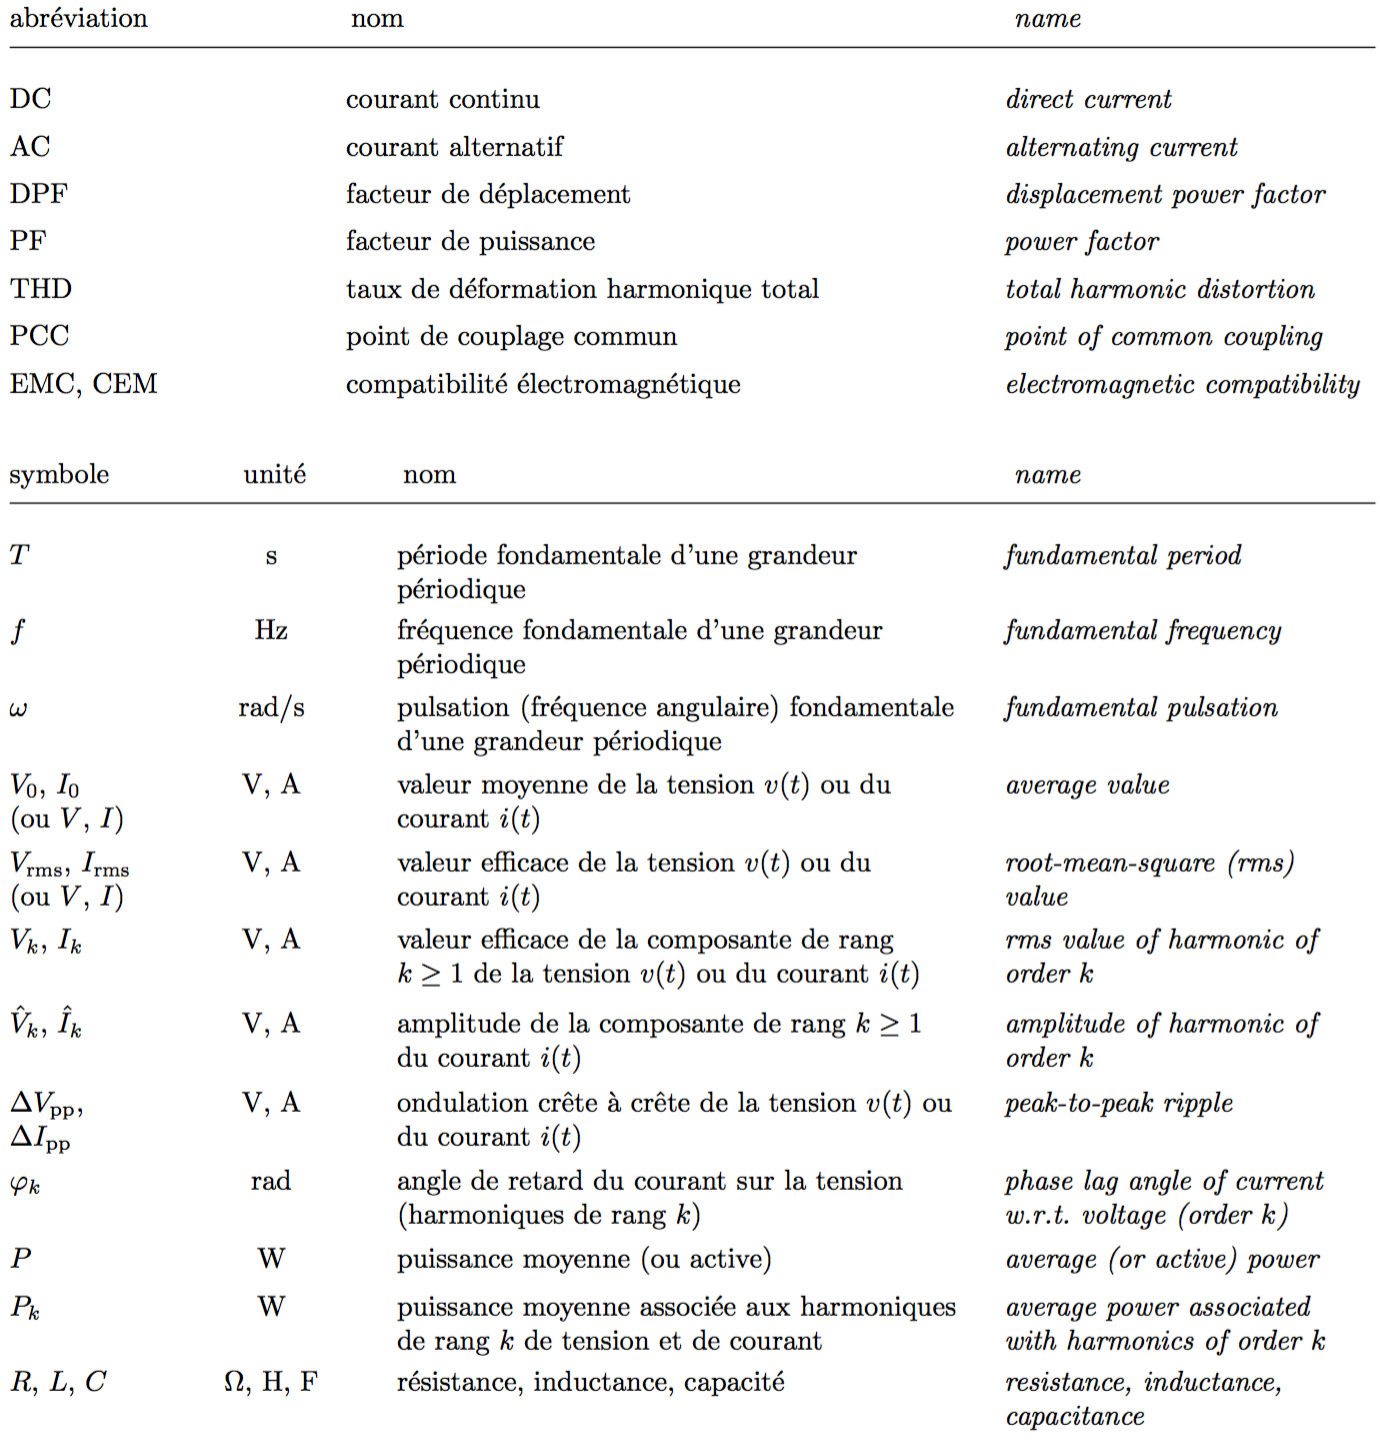
\includegraphics[scale=0.65]{ch1/1}
		\captionof{table}{List of abbreviations and symbols.}
		\label{table:1.1}
	\end{center}
	
	In the previous page, there's a table with abbreviations and symbols used in this chapter.
	The difference between power electronics and signal electronics is the high power consumption. We will focus on the conversion from one form of energy to another and not on signal transmission and analysis. In this course, we will study converters working at steady state. The distortion of physical quantities will be a nuisance.
	
\section{Different types of converters, semi-conducting components and applications}
	\subsection{Types of converters}
		Power electronics converters change properties of the electric energy between the input and the output. The different kinds of conversions and the corresponding converters relevant to this course are in \autoref{table:1.2}.
		
		We should remark the fact that converters are reversible when it comes to power, that is to say electric power can flow from the input to the output and conversely. The choice of the input will therefore depend on the main direction of the power flux for a given converter or application. This property is natural for electromagnetic converters (e.g. transformers) but it is not respected by static converters. This kind of converters contain semi-conducting components, which are non-linear, as well as magnetic components and capacitors.
		

		\begin{center}
			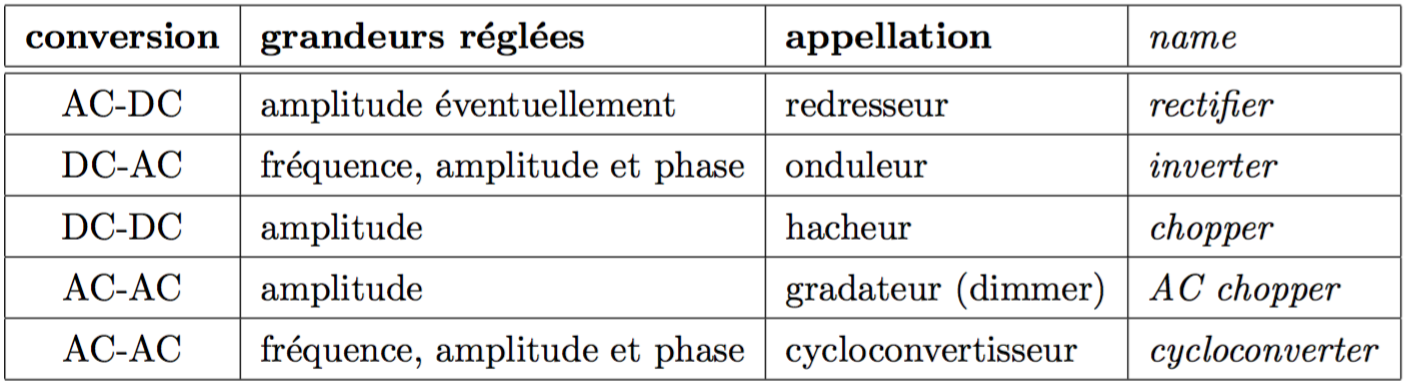
\includegraphics[scale=0.5]{ch1/2}
			\captionof{table}{Types de convertisseurs.}
			\label{table:1.2}
		\end{center}
		
	\subsection{Types of semi-conducting components}
	    We can classify the semi-conducting components according to their controllability: 

		\begin{itemize}
			\item[•] \textbf{Diodes} are non-linear and uncontrollable components. They are equivalent to a short-circuit following one direction and to an open circuit following the other direction. \textbf{Uncontrolled rectifiers} composed of diodes are widely employed. \\
			Frequency capacity: small to big.
			Power capacity: small to big.\\
			
			\item[•] \textbf{Thyristors} hold multiple diodes and a control electrode which allows the delay of the conduction but not the stop of the current. That is why they are called \textbf{semi-controllable.}  With \textbf{thyristor rectifiers}, we can control the output voltage and we can inverse it as well. They are also present in \textbf{AC choppers} and \textbf{cycloconverters}. Thyristors are \textbf{unidirectional} when it comes to current as diodes are.\\
			Frequency capacity: small.
			Power capacity: big.\\
			
			\item[•] The  \textbf{triac} is very similar to the thyristor because it is \textbf{semi-controllable}. However, it is \textbf{bidirectional} for the current too. That is because of the presence of two thyristors set in anti-parallel. We use them to compose \textbf{AC choppers}.\\
			Frequency capacity: small.
			Power capacity: small.\\
			
			\item[•] The last category of semi-conducting components comprises the fully controllable components. They are the \textbf{power transistors} (BJT, IGBT, MOSFET, ...) and components derived from the thyristor (GTO). We also call them \textbf{controllable switches}. They can be found in \textbf{universal bridges}. We call them universal because they can effect various energy conversions. \\
			In the order GTO - BJT, IGBT, ... - MOSFET, frequency capacity: small - medium - big, power capacity: big - medium - small. 
		\end{itemize}
		
	\subsection{Types of applications}
		\begin{wrapfigure}[9]{l}{3.7cm}
		\vspace{-5mm}
		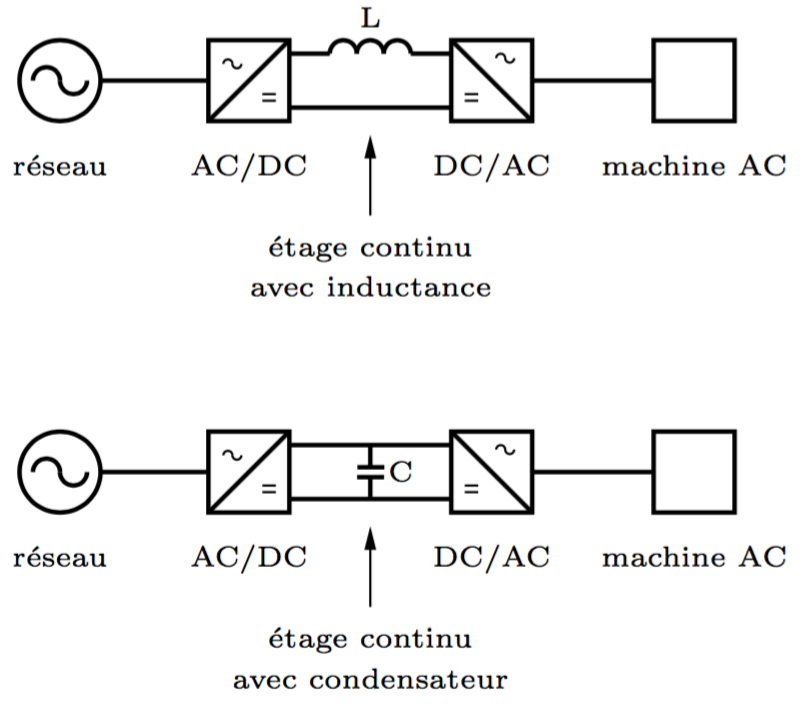
\includegraphics[scale=0.25]{ch1/4}
		\captionof{figure}{}
		\end{wrapfigure}	
		The AC-AC conversion is widely employed, in particular for the supply and control of AC electric machines. AC choppers and cycloconverters do this in only one step but they are very limited. The concatenation of an AC-DC converter and a DC-AC converter, with a capacitor (in parallel) or a self (in series) between them working as an energy limiter, will give more flexibility. We do the same thing for a DC machine by using a DC-DC converter instead of the DC-AC converter.
		
		\ \\
		\begin{wrapfigure}[8]{r}{3.5cm}
		\vspace{0mm}
		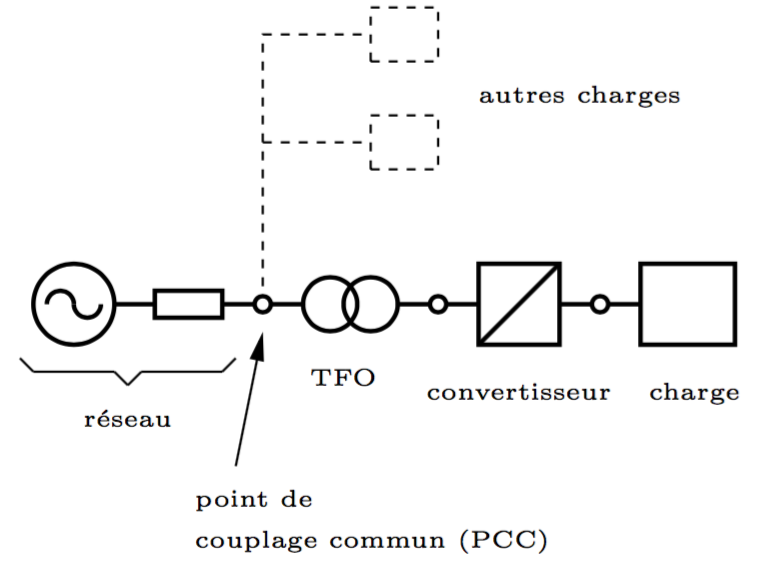
\includegraphics[scale=0.25]{ch1/5}
		\captionof{figure}{}
		\end{wrapfigure}
		
		A converter can be plugged into the grid if we put a transformer as an intermediary step. Depending on the type of converter and the load, a current more or less distorted is obtained as a result. As the supply has an inner impedance, the distorted voltage appear at the PCC (Point of Common Coupling). That might induce problems and damages in the other loads. That happens when the load has a bad \textbf{electromagnetic compatibility} (EMC). The problem of harmonics can be fixed by using \textbf{passive filters} (capacitors and inductors) or \textbf{active filters} (controllable converters).\\
		
		Another relevant aspect is the \textbf{reactive power} of the network (AC network) and/or of the load (AC load). Some converters can supply reactive power instead of pulling a current retarded with respect to the voltage. This is crucial for asynchronous machines working as loads because they consume reactive power. The reversibility of the active power consumption of the converter is equally important. For example, the recovery of electric power from the braking or its dissipation in a resistance. 
		

\section{Periodic regimes and harmonics}
	\begin{wrapfigure}[6]{l}{5cm}
	\vspace{-5mm}
	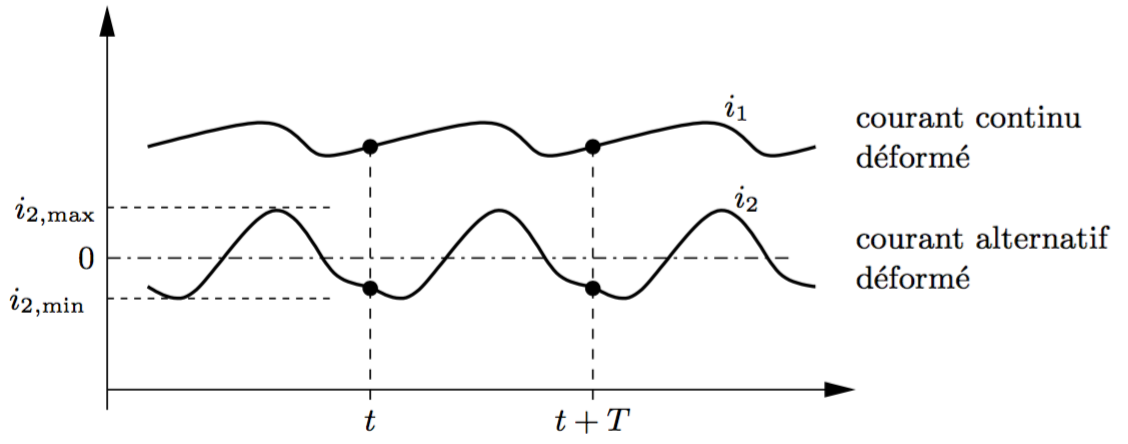
\includegraphics[scale=0.25]{ch1/6}
	\captionof{figure}{}
	\end{wrapfigure}
	
	In this course, when studying converters we will focus on steady-state operating conditions. Currents and voltages are therefore periodic functions where the fundamental period is designed by $T$. In the figure, the first signal can be designed as continuous because it remains positive and the continuous component is dominating whereas the second one is considered as an alternative signal even if it has a continuous component. The peak-to-peak ripple is the difference between the maximum and the minimum value of the signal. The fundamental frequency $f = 1/T$ is directly linked to the frequency of the power supplied to the converter, or to the controlled cutting frequency. The presence of non-linear components and the cutting of the switches distort the signals.

		
	\subsection{Fourier analysis}
	If we consider a periodic function $i(t)$ whose fundamental pulsation is $\omega = 2\pi f = 2\pi /T$, its decomposition is given by:

	\begin{equation}
	\begin{aligned}
		i(t) &= I_0 + \sum _{k\geq 1} \left(Î_{ck} \cos k\omega t + Î_{sk} \sin k\omega t\right)\\
			&= I_0 + \sum _{k\geq 1} \underbrace{Î_k \cos (k\omega t +\gamma _k)}_{i_k(t)} \qquad with \qquad Î_{ck} - jÎ_{sk} = Î_k e^{j\gamma _k},
	\end{aligned}
	\end{equation}
	where $I_0$ is the continuous component and $i_k(t)$ is the rms value of harmonic of order k. The continuous component gives the average value of $i(t)$ over a fundamental period because the average value of each harmonic is equal to zero: 
	\begin{equation}
		I_0 = \frac{1}{T}\int _0 ^T i(t)\, dt
	\end{equation}
	The orthogonality equation from page 7 of the syllabus furnishes the following relations for $k\geq 1$ : 
	\begin{equation}
	\begin{aligned}
		Î_{ck} &= &Î_k \cos \gamma _k &= \frac{2}{T} \int _0 ^T i(t) \cos k\omega t\, dt\\
		Î_{sk} &= &-Î_k \sin \gamma _k &= \frac{2}{T} \int _0 ^T i(t) \sin k\omega t\, dt
	\end{aligned}
	\end{equation}
	
	The \textbf{half-wave symmetry} manifests itself very often in practical cases. By definition there is half-wave symmetry when $v(t) = -v(t+T/2)$ or $i(t) = -i(t+T/2)$. This allows us to neutralize even-order harmonics: 
	\begin{equation}
		\int _0 ^T v(t)\cos k \omega t \, dt = \frac{1}{T}\int _0 ^{T/2} v(t) \underbrace{\left(\cos k\omega t - \cos k\omega(t+T/2)\right)}_{\mbox{= 0 if k is even}}\, dt
	\end{equation}
	
	\subsection{Root-mean-square (rms) value}
		The rms value of the current $i(t)$ is given by:
		\begin{equation}
			I_{rms} = \sqrt{\int _0 ^T i^2(t) \, dt} = \sqrt{I_0^2 + \frac{1}{2}\sum _{k\geq 1}Î_k ^2 } = \sqrt{I_0^2 + \sum _{k\geq 1} I_k^2},
		\end{equation}
		where $I_k = \frac{1}{\sqrt{2}}Î_k$ is the rms value of harmonic of order $k$. The product of harmonic components of different orders $I_kI_l$ doesn't appear because of their orthogonality. If we consider the current flowing through a resistance $R$, the \textbf{Joule losses} are $Ri^2(t)$ and the \textbf{average power over a fundamental period T} is given by:
		\begin{equation}
			P_J = \frac{1}{T}\int _0^T Ri^2 \, dt = RI_0^2 + \sum _{k\geq 1} RI_k^2 = RI_{rms}^2,
		\end{equation}
		and they are therefore proportional to the square of the rms value of the current.

		
	\subsection{Instantaneous and average electrical power}
	    If we consider a voltage $v(t)$ and a current $i(t)$, both periodic of period T:
		\begin{equation}
			v(t) = V_0 + \sum _{k \geq 1} \underbrace{\sqrt{2} V_k \cos (k\omega t+ \gamma _{vk})}_{v_k(t)} \qquad and \qquad
			i(t) = I_0 + \sum _{k \geq 1} \underbrace{\sqrt{2} I_k \cos (k\omega t+ \gamma _{ik})}_{i_k(t)}
		\end{equation}
		The instantaneous power associated to them is given by $p(t) = v(t)i(t)$ and the average power
		\begin{equation}
			P = \frac{1}{T}\int _0 ^T p(t)\, dt = \underbrace{V_0I_0}_{P_0} + \underbrace{V_1I_1\cos \varphi _1}_{P_1} + \sum _{k\geq 2}\underbrace{V_kI_k \cos \varphi _k}_{P_k}
			\label{eq:1.8}
		\end{equation}
		where $P_0$ is the power associated to the continuous component, $P_k$ to the harmonic of order $k\geq 1$ and where $\varphi _k = \gamma _{vk} - \gamma _{ik}$ is the phase lag angle of current with respect to voltage (order k). Once again the product of different order of harmonics doesn't appear. The addition in \eqref{eq:1.8} can be limited to a single term:
		\begin{itemize}
			\item[•] If the voltage $v(t)$ is continuous and not distorted ($v(t) = V_0; V_k = 0, k\geq 1$) the average power is given by $P = V_0I_0$ for any possible current. The same happens when we inverse current and voltage. 
		 
			\item[•] If the voltage is sinusoidal and not distorted ($v(t) = \sqrt{2}V_1\cos (\omega t + \gamma _v); V_k = 0, k\neq 1$), the average power is given by $P = V_1I_1\cos \varphi _1$ for any possible current. The same happens when we inverse current and voltage. 
			
		\end{itemize}
		Anyways, $P_k$ often remains negligible with respect to $P_0$ or $P_1$. 
		
	\subsection{DC quantities}
	In absence of distortion, the DC quantities are constant. The distortion of the current $\Delta i(t)$ can comprise all the harmonics of order $k\geq 1$ : 
		\begin{equation}
			i(t) = I_0 + \underbrace{\sum _{k\geq 1} Î_k \cos (k\omega t +\gamma _k)}_{\Delta i(t)}
		\end{equation}
		The rms value of the distortion $\Delta i(t)$ is given by: 
		\begin{equation}
			\Delta I_{rms} = \sqrt{\frac{1}{2}\sum _{k\geq 1} Î_k^2} = \sqrt{\sum _{k\geq 1} I_k^2}
		\end{equation}
		The rms value of the current can therefore be written differently: 
		\begin{equation}
			I_{rms} = \sqrt{I_0^2+\Delta I^2_{rms}}.
		\end{equation}
		The supplementary Joule losses induced by the distortion are given by $R(\Delta I_{rms})^2$. 
		
	\subsection{Sinusoidal quantities (single phase systems)}
	    When there's no distortion, the AC quantities are perfectly sinusoidal. The distortion, if there's any, manifests itself as a continuous component $I_0$ and harmonics of order $k\geq 2$ :
		\begin{equation}
			i(t) = \underbrace{Î_1\cos (\omega t+\gamma _1)}_{i_1(t)} + \underbrace{I_0 + \sum _ {k\geq 2} Î_k \cos (k\omega t + \gamma _k)}_{\Delta i(t)}
		\end{equation}
		The rms value of the distortion is given by: 
		\begin{equation}
			\Delta I_{rms} = \sqrt{I_0^2+\frac{1}{2}\sum _{k\geq 2} Î_k^2} = \sqrt{I_0^2+ \sum _{k\geq 2} I_k^2}
		\end{equation}
		The \textbf{THD - Total Harmonic Distortion} of an AC quantity is defined as the ratio of the rms value of the distortion and the rms value of the fundamental component:
		\begin{equation}
			THD = \frac{\Delta I_{rms}}{I_1}
		\end{equation}
		The \textbf{DPF - Displacement Power Factor} is defined as the cosine of the angle $\varphi _1$ (the phase lag angle of the fundamental component of the current w.r.t. the fundamental component of the voltage): 
		\begin{equation}
			DPF = \cos \varphi _1.
		\end{equation}
		The \textbf{apparent power S} and the \textbf{PF - Power Factor} are defined as:
		\begin{equation}
			S = V_{rms}I_{rms} \qquad and \qquad PF = \frac{P1}{S} = \frac{V_1I_1\cos \varphi _1}{V_{rms}I_{rms}}
		\end{equation}
		where $P_1$ is the average (or active) power associated with fundamental harmonics. The PF is almost always smaller to 1 because of the phase lag $\varphi _1$ or the distortion of either the voltage or the current ($V_{rms}>V_1$ or $I_{rms}>I_1$). For AC power transmission, a load is considered ideal if, when it is plugged into a perfect sinusoidal voltage source, the absorbed current is perfectly sinusoidal, the resistance is constant and there's no phase shift. When this happens the DPF and the PF are equal to 1. The Joule losses and the rms value of the current are minimal when that happens. 
		
		\subsubsection{Square-wave and triangular current}
			\begin{center}
			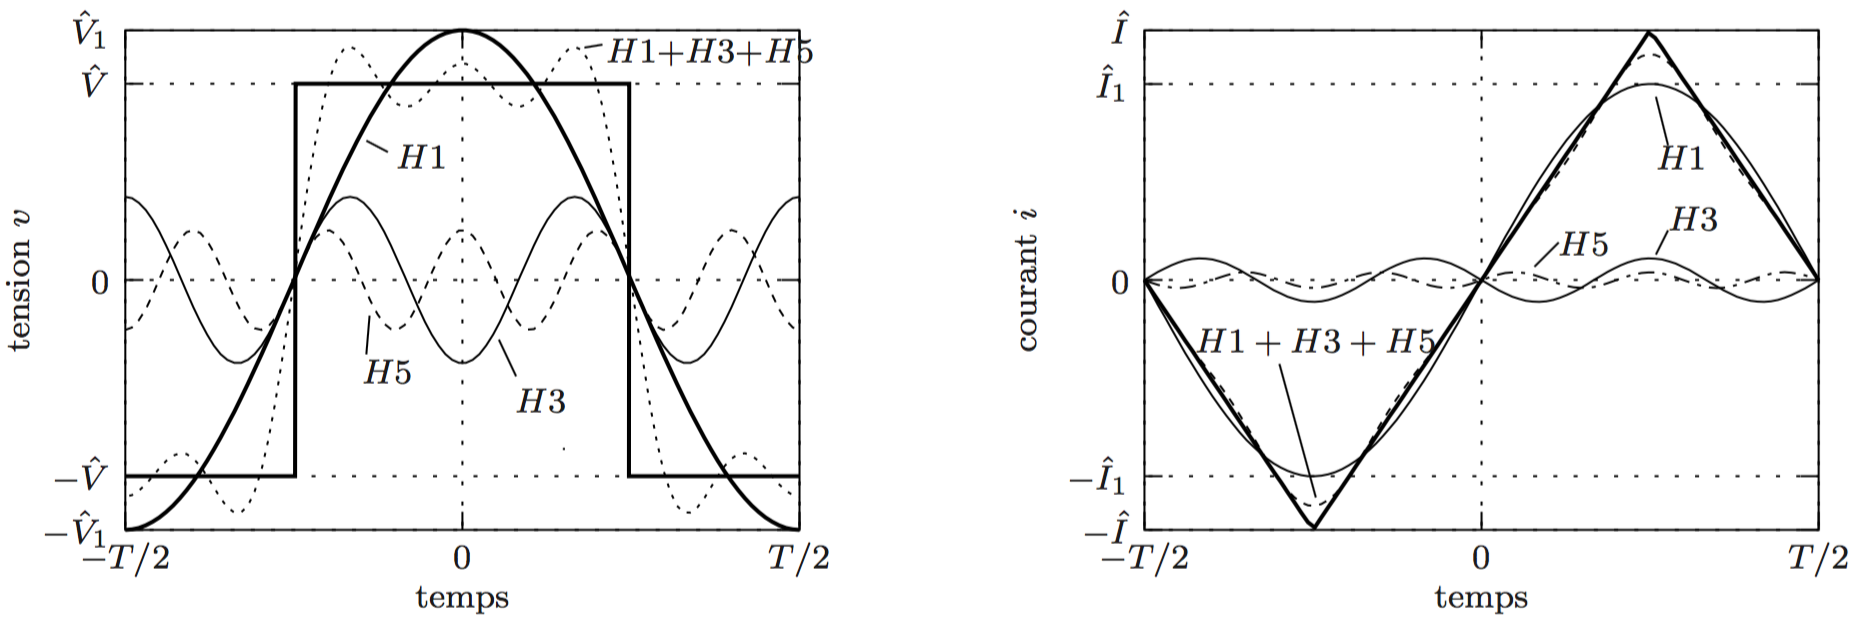
\includegraphics[scale=0.4]{ch1/7}
			\captionof{figure}{}
			\end{center}
			According to the figure, the square-wave voltage $v(t)$ fluctuates between $\hat{V}$ and $-\hat{V}$. The amplitude and the rms value of the fundamental period are given by: 
			\begin{equation}
				\hat{V}_1 = \frac{4}{\pi}\hat{V} \qquad and \qquad V_1 = \frac{2\sqrt{2}}{\pi} \hat{V}
			\end{equation}
			As even order harmonics are absent of the spectre because of the half-wave symmetry and the amplitude of harmonic of order $k\geq 1$ is inversely proportional to their order $\hat{V}_k = \frac{1}{k}\hat{V}_1$: 
		   	\begin{equation}
		   		THD = \sqrt{1/3^2 + 1/5^2+1/7^2+ \dots} = 48.3\%
		   	\end{equation}
			In order to obtain a \textbf{triangular current}, we impose a square-wave voltage $v(t) = \pm \hat{V}$ to a self of inductance L. As a result, we obtain a triangular current of gradient $\frac{di}{dt}= \pm \frac{1}{L}\hat{V}$. The half-wave symmetry appears in this wave too and the odd order harmonics are linked together as follows:
		   	\begin{equation}
		   		\hat{V}_k \cos (k\omega t+ \gamma _k) = L\frac{d}{dt}\left( Î_k \sin (k\omega t+ \gamma _k)\right)\qquad \Rightarrow  \hat{V}_k = k\omega L Î_k
			\end{equation}		  
			Therefore, the amplitude of harmonics of odd orders $k\geq 1$ are $Î_k = \frac{1}{k^2}Î_1$. The current is less distorted than the voltage:
			\begin{equation}
				THD = \sqrt{1/3^4+1/5^4+1/7^4+\dots} = 12.12\%
			\end{equation}
			We can study the analogous case by imposing the flow of a square wave current through a capacitor. The slope of the triangular voltage is given by $\frac{dv}{dt} = \pm \frac{1}{C}Î$ and the harmonics are linked together as follows: 
		   	\begin{equation}
		   		Î_k = k\omega C \hat{V}_k.
		   	\end{equation}
		   	
	\subsection{Three-phase square-wave}
		\subsubsection{Arbitrary periodic regime}
		Let's consider 3 currents $i_a(t)$, $i_b(t)$ and $i_c(t)$, with the same fundamental period T. That's a three-phase system if three quantities are equal but they have a shift equal to $\pm T/3$, for \textbf{direct phase order} and \textbf{inverse phase order} that means:
		\begin{equation}
			i_a(t) = i_a(t+T/3) = i_a(t-T/3) \qquad and \qquad i_a(t) = i_a(t-T/3) = i_a(t+T/3)
		\end{equation}
		
		The signal is called \textbf{homopolar} when all the currents are identical. When it comes to \textbf{harmonic content}, for a direct order system with half wave symmetry (no even harmonics), the order $k$ of the remaining harmonics can be written as $k = 6m+1, k = 6m +3, k= 6m+5$ ($n \in Natural$ numbers). The expressions of the currents are developed as follows: 
		\begin{equation}
			i_a(t) = \sum _{k = 6m+1}Î_{a,k} \cos (k\omega t + \gamma _{a,k})+ \sum _{6m+3}Î_{a,k} \cos (k\omega t + \gamma _{a,k}) + \sum _{6m+5}Î_{a,k} \cos (k\omega t + \gamma _{a,k})
		\end{equation}
		
		Symmetry is also of application for harmonics, then the amplitude of the current is the same for all the phases. In order to find the relation between the phase angles we will exploit the direct phase order properties:
			\begin{equation}
				\cos (\omega t + \gamma _{a,k}) = \cos (\omega t + \gamma _{b,k} + \frac{2\pi}{3}) = \cos (\omega t + \gamma _{c,k} - \frac{2\pi}{3}). 
			\end{equation}
			\begin{itemize}
				\item[•] If $k = 6m+1 :$\\
				We obtain $\gamma _{a,k} = \gamma _{b,k} + \frac{2\pi}{3} = \gamma _{c,k} - \frac{2\pi}{3}$. The harmonics form a direct phase order three-phase system of period $T/k$. 
				\item[•] If $ k = 6m+3 :$\\
				We obtain $\gamma _{a,k} = \gamma _{b,k} = \gamma _{c,k}$. This corresponds to homopolar systems $k = 3, 9, ...$.when the addition of the phases equals 0 at any time, $i_{a,k}(t)+i_{b,k}(t)+i_{c,k}(t) = 0$. Harmonics multiples of 3 are therefore eliminated. 
				\item[•] If $k = 6m+5$\\
				We obtain $\gamma _{a,k} = \gamma _{b,k} -\frac{2\pi}{3} =\gamma _{c,k}+\frac{2\pi}{3}$. These harmonics correspond to inverse phase order three-phase systems. 
				 \newpage
			\end{itemize}
			
		\subsubsection{Three phase square wave}
			\begin{wrapfigure}[9]{l}{4cm}
			\vspace{-5mm}
			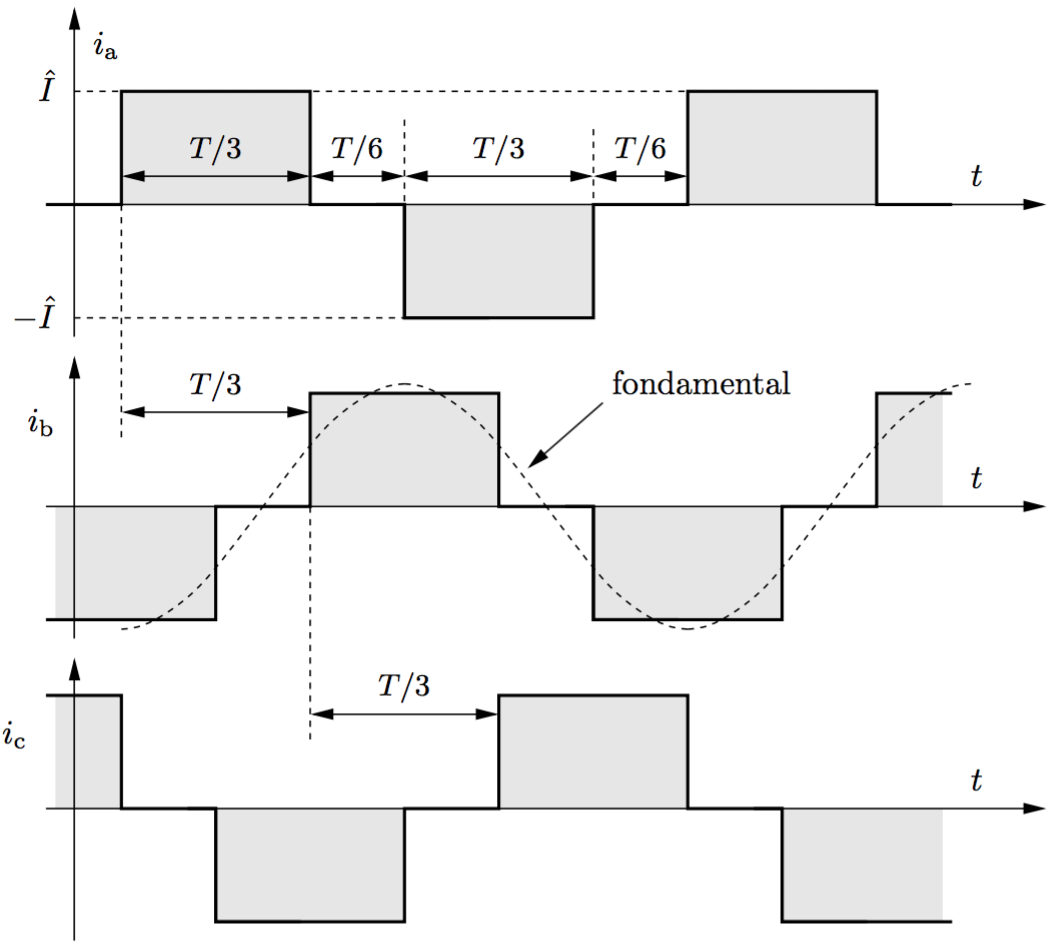
\includegraphics[scale=0.20]{ch1/8}
			\captionof{figure}{}
			\end{wrapfigure}		
			In the figure we observe easily the direct order symmetry existent between the currents (of fundamental period $T$). The impulsions of period $T/3$ are separated by intervals of length $T/6$. The amplitude and the rms value of the current are given by:
			\begin{equation}
				Î_{1} = \frac{2\sqrt{3}}{\pi} Î \qquad and \qquad I_1 = \frac{\sqrt{6}}{\pi} Î.
			\end{equation}
			There's only odd order harmonics (half-wave symmetry) and harmonics of orders divisible by 3 are also excluded (homopolar components). The components of the current are $Î _k = Î_1/k$ and the THD is:
			\begin{equation}
				THD = \sqrt{1/5^2 + 1/7^2 + 1/11^2 / \dots} = 31.1\%
			\end{equation}
			
	\subsection{Zero average voltage across an inductance and zero average current in a capacitor}
		\subsubsection{Inductance}
		If the signal is at steady state and has a period $T$, the average voltage $V_{L,0}$ equals 0 (for a constant inductance) :
			\begin{equation}
				V_{L,0} = \frac{1}{T}\int _{t_0}^{t_0+T} v_L (t)\, dt = \frac{L}{T}\int _{t_0}^{t_0+T} \frac{di_L}{dt}\, dt = \frac{L}{T}\left(i_L(t_0 + T) - i_L(t_0)\right) = 0
			\end{equation}
		The same thing happens in the case of a non linear inductance if we are in steady state because the flux is periodic $\phi _L(T+t_0) = \phi _L (t_0)$ and $v_L = \frac{d\phi _L}{dt}$. In steady state, the inductance absorbs and debits magnetic energy alternatively according to the expression $e_L(t) = \frac{1}{2} Li_L^2$. The current fluctuates around its average value $I_{L,0}$ and the energy fluctuates around $E_{L,0}=\frac{1}{2} L I_{L,rms}^2$ at twice the fundamental frequency. 
			
		\subsubsection{Capacitor}
		At steady state, a periodic signal of period $T$ has an average current equal to 0 for a constant capacity $C$ : 
		\begin{equation}
			I_{C,0} = \frac{C}{T}\int _{t_0}^{t_0+T} \frac{dv_C}{dt} \, dt = \frac{C}{T} (v_{C}(t_0+T)-v_C(t_0)) = 0
		\end{equation}
		
		The electric energy collected between the electrodes of the capacitor is $e_C(t) = \frac{1}{2}Cv^2_C$. It debits and absorbs power alternatively, where the voltage oscillates around $V_{C,0}$ while the energy oscillates around $E_{C,0} = \frac{1}{2} C V_{C,rms}^2$. 
%%%%%%%
% Ch2 %
%%%%%%%

\chapter{Diode rectifiers}
	
	Diode rectifiers are simple and cheap and they don't need any adjustment prior to their employment. They provide a DC voltage primarily constant from an AC voltage. There are two kinds of load to supply: those who need a smooth DC voltage and those who need a limited voltage distortion. Electronic devices belong to the first category, that's why we find capacitors connected between the output terminals. Those capacitors will smooth the rectified signal. DC machines and RLE loads belong to the second category. They need thyristor rectifiers (\textbf{controllable}) because the diode rectifier is uncontrollable.
	The list of symbols needed in this chapter is just below.
	
	\begin{center}
	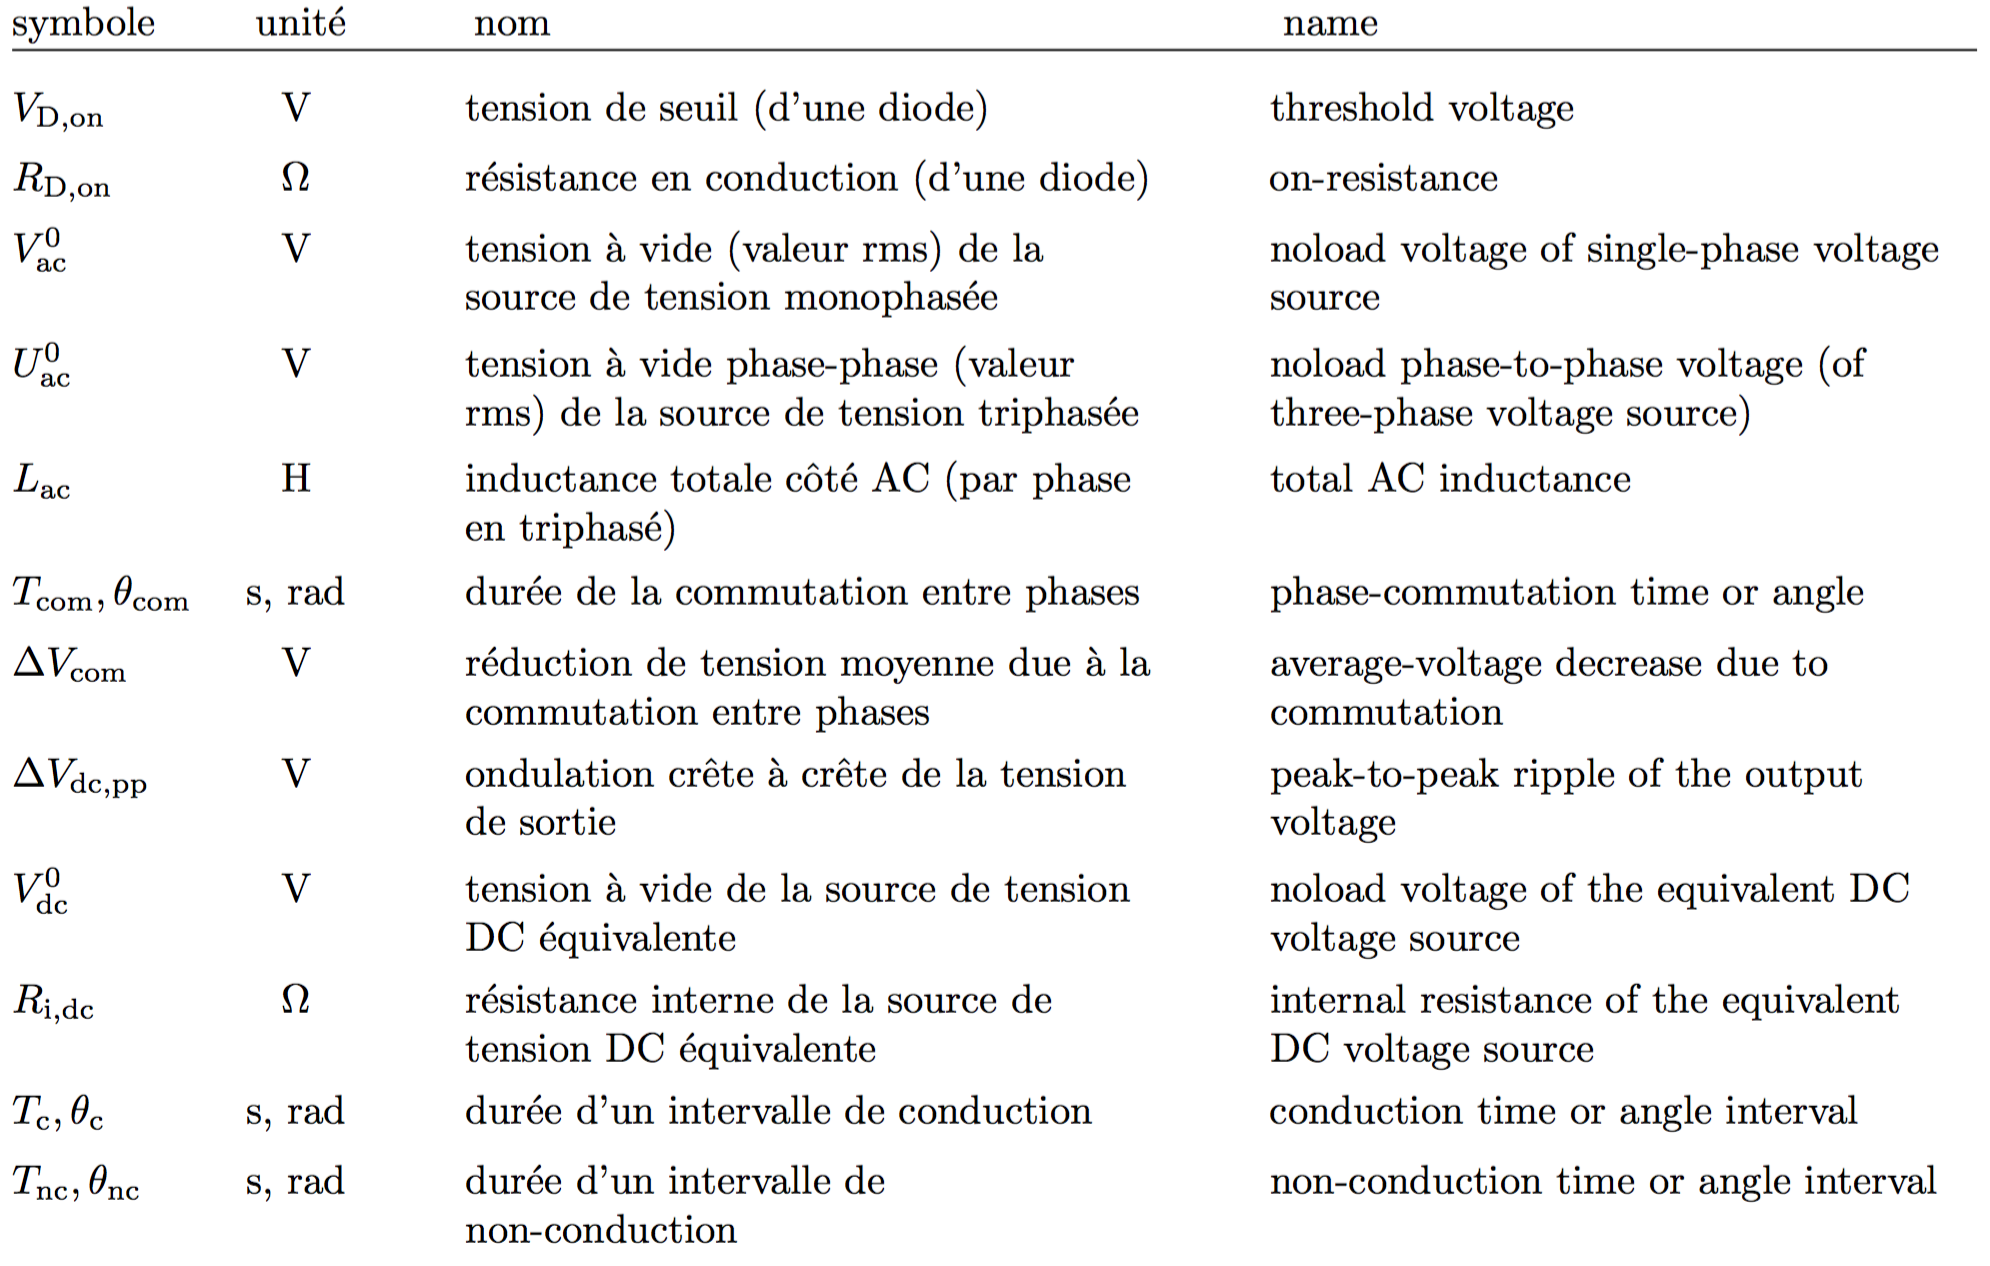
\includegraphics[scale=0.45]{ch2/1}
	\captionof{table}{List of symbols.}
	\end{center}
	\newpage
	
	\section{Characteristics of diodes}
		This figure shows the symbol of a diode as well as three characteristics depending on the accuracy needed. The diode \textbf{conducts} if $v_D=v_{AK}$ (\textbf{threshold voltage}). Voltage will therefore barely depend on current $i_D$.
		
		\begin{center}
		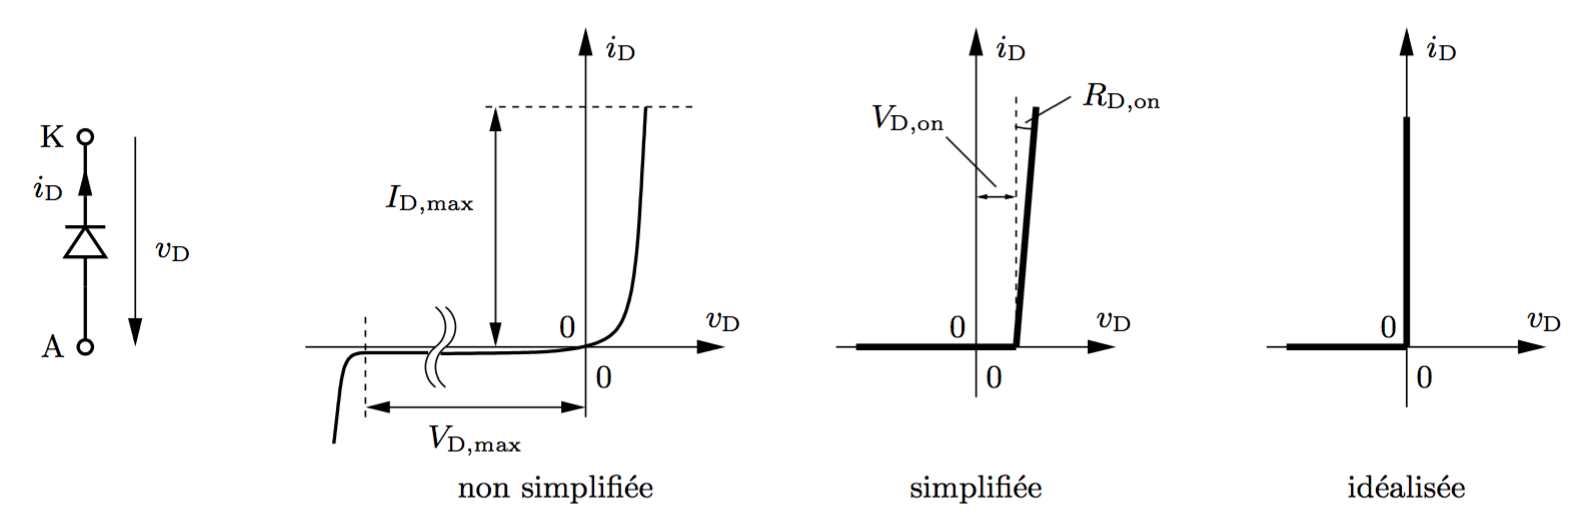
\includegraphics[scale=0.45]{ch2/2}
		\captionof{figure}{}
		\end{center}			
		
		The maximum current admitted by a diode (during long intervals of time) represented by $I_{D,max}$ in the figure depends on its construction, its size and its cooling system and it can reach up to some kA.
		Heat transfer to the radiator is essential in the conception and employment of power electronics diodes. As other semi-conducting components, diodes have little thermal inertia because of their size. Its temperature can therefore rise very fast.
		According to the simplified characteristic, conduction losses are approximated as follows:
		
		\begin{equation}
			v_D = V_{D,on} + R_{D,on} i_D
		\end{equation}
		where $V_{D,on}$ is the \textbf{threshold voltage} and is approximately $1V$. Besides low voltage applications (less than 10 volts), we will neglect this voltage $v_D$ because it has little influence on the characteristics of diode integrated converters. However, we will not forget the fact that the voltage drop corresponds to the instantaneous conduction losses $P_D(t) = v_D(t)i_D(t)$ and the evacuation of these losses is essential. \\
	
        In power electronics, diodes are used at low commutation frequencies ($50 - 60 Hz$).
	
	\section{Inductive load and elementary rectifiers}
		\subsection{Elementary rectifier circuits, generic RLE load}
		In order to study some elementary circuits employing one or two diodes and other circuits such as diode bridges, we will consider a generic RLE load. R, L and E are constant, which means that their variation over a fundamental period of the AC source is arbitrarily small. Such a load might represent, for example, the induced circuit of a DC machine ($E_{dc} \neq 0$) or its excitation circuit ($E_{dc}=0$). The differential equation of the voltage over the load is:
		\begin{equation}
			v_{dc} = E_{dc} + R_{dc}i_{dc} + L_{dc}\frac{di_{dc}}{dt}.
		\end{equation}
			
		At steady state and by introducing the \textbf{average voltage} $V_{dc}$ and the \textbf{average current} $I_{dc}$, we get:
			
			\begin{equation}
				V_{dc} = E_{dc} + R_{dc} I_{dc}.
			\end{equation}
			
			The load is fed by a diode rectifier, thus $i_{dc}$ and $I_{dc}$ cannot be negative and if $E_{dc}\geq v_{ac}$ then the current stops flowing. We can therefore write:
			\begin{equation}
				I_{dc} = max\left(\frac{V_{dc} - E_{dc}}{R_{dc}}, 0\right).
			\end{equation}
			The inductance of the load will smooth the current. This effect will be greater as the time constant $\tau = L_{dc}/R_{dc}$ becomes greater with respect to the period $T=1/f$ of the grid. For single-phase bridges and three-phase bridges the period concerning us will be $T/2$ and $T/6$ respectively. In the case of an MCC, the fluctuations of the voltage imposes a fluctuation of the current and, therefore, a fluctuation of the \textbf{electromagnetic torque}, which is troubling. Thus, we can add an outer inductance if the inner one is not enough, at the expenses of losing dynamic performance. 

		\subsection{Elementary rectifier circuit with an RE load}
			\subsubsection{With an R load}
			    We will begin by analyzing the simpler case, the one of an R load. The figure hereafter represents a circuit with an AC ideal voltage source of frequency $f$ linked to an ideal diode and a resistance $R_{dc}$. In this case, $i_{ac}(t)=i_{dc}(t)$. The diode isn't in direct bias unless $v_{ac}(t)>0$. When that happens we have $v_{dc}(t)=v_{ac}(t)$ and $i_{dc}=v_{ac}(t)/R_{dc}$. The diode will stop the current when $v_D=v_{ac}<0$, and we will have $v_{dc}=0=i_{dc}$.
				
				\begin{center}
					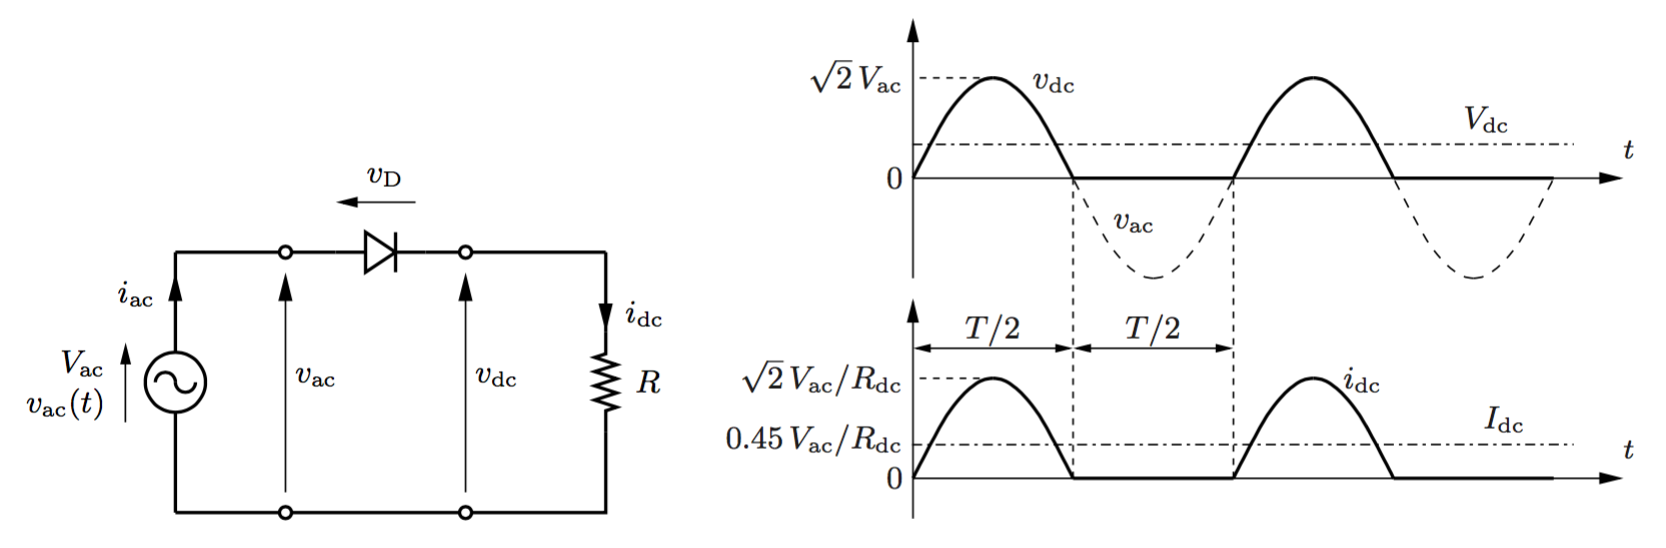
\includegraphics[scale=0.45]{ch2/3}
					\captionof{figure}{}
				\end{center}
				
				We obtain the average value of the voltage by integrating the instantaneous voltage over half a conduction period:
				\begin{equation}
					V_{dc} = \frac{1}{2\pi} \int _0^\pi \sqrt{2}V_{ac}\sin (\omega t) \, d\omega t = \underbrace{\frac{\sqrt{2}}{\pi}}_{0.450} V_{ac}.
					\label{eq:2.5}
				\end{equation}
				
				The rectified voltage and its respective current $i_{dc}=i_{ac}$ are highly distorted, all the harmonics of frequency $kf$ are present (we don't have half-wave symmetry). This circuit is not very appropriate for practical cases. In addition, having a DC current come from an AC source will generate problems. 
				
			\subsubsection{With an RE load}
			
			    Now we have a DC voltage source added to the load. It might be the case of a battery and its inner resistance. 
				
				\begin{center}
				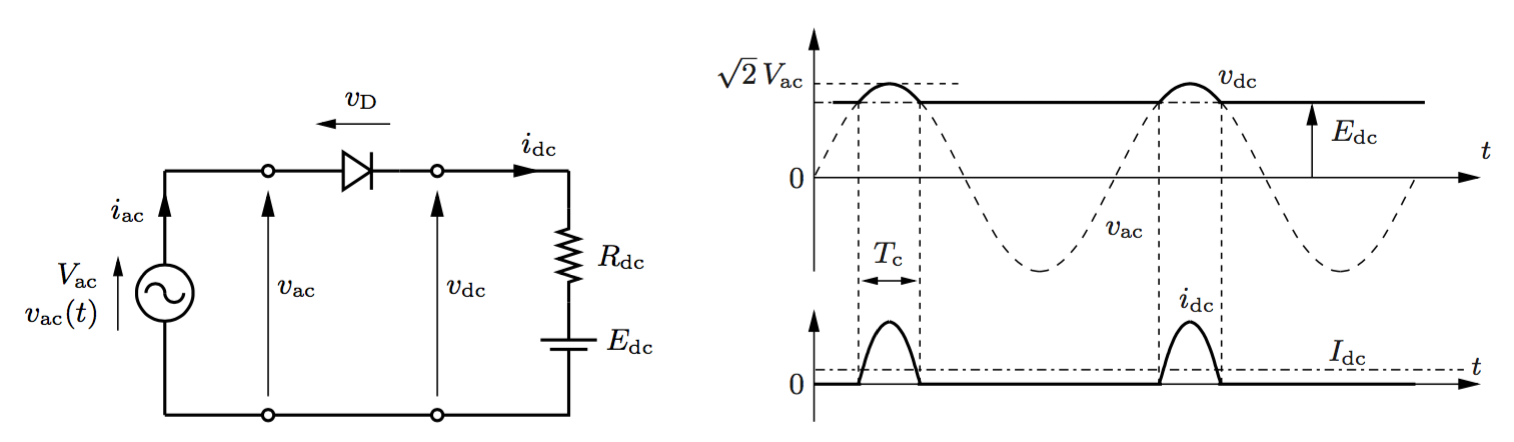
\includegraphics[scale=0.45]{ch2/4}
				\captionof{figure}{}
				\end{center}	
				
				When the diode conducts we have: $v_{ac}(t) = v_{dc}(t) = E_{dc} + R_{dc}I_{dc}$. This happens if the condition $(v_{ac}-E_{dc})/R_{dc}>0$ (that is to say $v_{ac}>E_{dc}$) is respected. When the diode blocks the passage of the current we have $v_{dc} = E_{dc}$. The DC quantities are distorted and every harmonic of frequency $kf$ will appear in the spectre.
				The conduction intervals will have an extension $T_c$ where $\theta _c = \omega T_c$. Its duration can be calculated as follows:
				\begin{equation}
					E_{dc} = \hat{V}_{ac} \sin \left(\frac{\pi}{2} - \frac{\theta _c}{2}\right) = \hat{V}_{ac} \cos \frac{\theta _c}{2} \qquad \Rightarrow \qquad \theta _c = 2 \arccos \frac{E_{dc}}{\hat{V}_{ac}}
				\end{equation}
				In this equation we can ascertain that as $E_{dc}$ grows closer to $\hat{V}_{ac}$ the extension of the intervals decreases. The average voltage $V_{dc}$ can be obtained by integrating over a conduction interval $\theta _c$ and the remaining $2\pi - \theta _c$ : 
				\begin{equation}
				\begin{aligned}
					\frac{V_{dc}}{\hat{V}_{ac}} &= \frac{1}{2\pi\hat{V}_{ac}} \left[ \int _0 ^{2 \arccos \frac{E_{dc}}{\hat{V}_{ac}}} \hat{V}_{ac} \sin \omega t\,  d\omega t + \int _{2 \arccos \frac{E_{dc}}{\hat{V}_{ac}}} ^{2\pi} E_{dc} \, d\omega t \right]\\
								&= \frac{1}{\pi} \sqrt{1 - \left(\frac{E_{dc}}{\hat{V}_{ac}}\right)^2} + \left(1- \frac{1}{\pi} \arccos \frac{E_{dc}}{\hat{V}_{ac}} \right)
				\end{aligned}
				\end{equation}
				
	\subsection{Elementary rectifier circuit with a free-wheeling diode}
		\begin{wrapfigure}[11]{l}{4.7cm}
		\vspace{-5mm}
		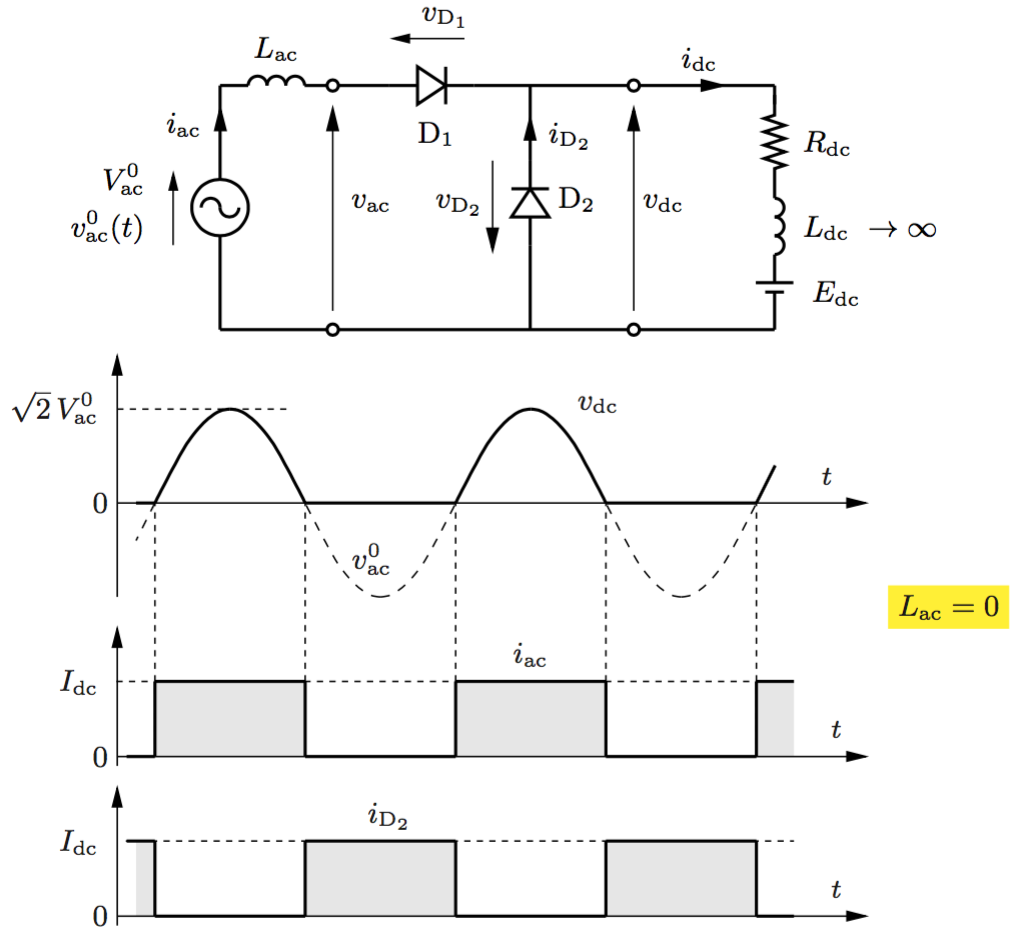
\includegraphics[scale=0.25]{ch2/5}
		\captionof{figure}{}
		\end{wrapfigure}
		In the figure we can observe two diodes D1 and D2, the first one will work the same way as before and the second one (free wheeling-diode) will be an extra path for the current going through the load to follow. The AC load is depicted by its equivalent without a load: a voltage source $v_{ac}^0(t)$ and an inner inductance $L_{ac}$.
		First we will consider the case where $L_{dc} \rightarrow \infty$. Such an inductance will perfectly smooth the current $i_{dc} = I_{dc}$. It remains a single track rectifier because the current is not alternative. 
		
		\ \\
		\subsubsection{Ideal AC voltage source and infinitely inductive load}
		
		    We will begin considering that the AC voltage source is ideal, that is to say $L_{ac} = 0$; and the DC inductance $L_{dc} = \infty$ : 
			\begin{equation}
				i_{dc}(t) = I_{dc} = i_{ac}(t) + i_{D2}(t)
			\end{equation}
			
			We can easily conclude that the load will be fed by the supply during positive alternations and by the free-wheeling diode during negative alternations. The commutation between the diodes is supposed to be instantaneous. The average value of the voltage can therefore be calculated as in \eqref{eq:2.5}. During negative alternations, as D2 lets the current pass, $-v_{D2} = v_{dc} = 0$ and all the voltage appears on D1.  
			
		\subsubsection{Non-ideal AC voltage source and infinitely inductive load}
			\begin{wrapfigure}[10]{l}{5.8cm}
			\vspace{-5mm}
			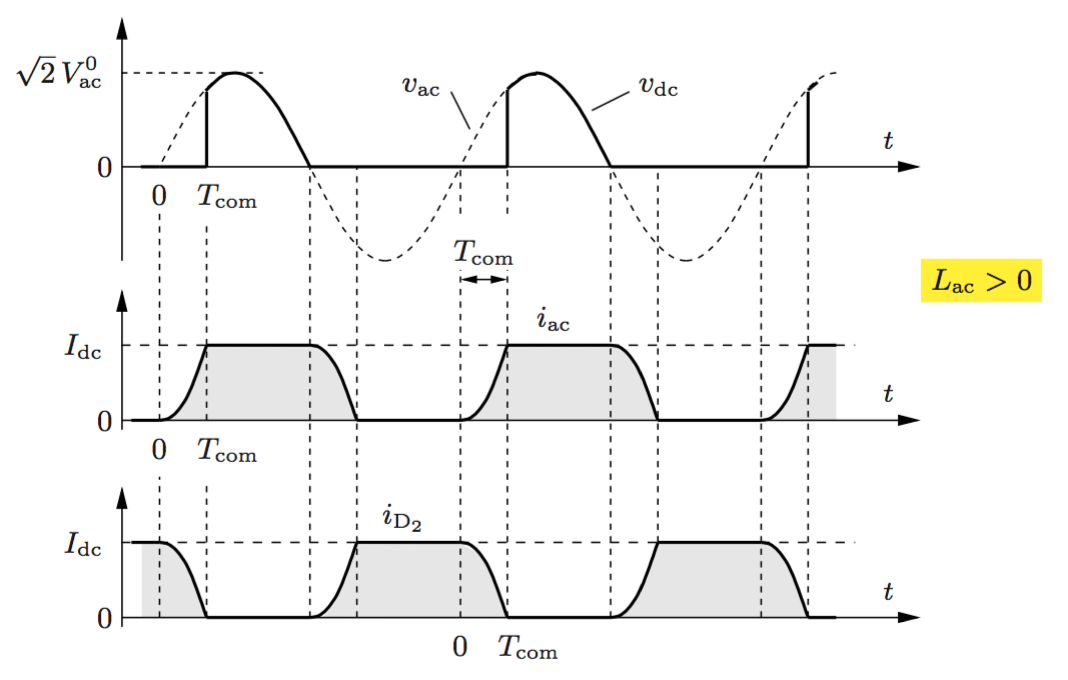
\includegraphics[scale=0.3]{ch2/6}
			\captionof{figure}{}
			\end{wrapfigure}
			Now, $L_{ac}$ prevents instantaneous variations of the current during commutations. The interval, referred to by $T_{com}$, during which both diodes conduct simultaneously can also be called \textbf{encroachment} or \textbf{overlapping} interval. The equation reigning over the commutation between diodes is:
			\begin{equation}
				v_{ac}^0 (t) = \sqrt{2} V_{ac}^0 \sin \omega t = L_{ac}\frac{di_{ac}(t)}{dt}.
				\label{eq:2.9}
			\end{equation}
			During these commutations, the output voltage \\$v_{dc}(t) = - v_{D2}(t) = 0$. In addition, as we consider an infinitely inductive load , the DC current is constant even during commutation intervals. That means: $i_{dc}(t) = I_{dc} = i_{D2}(t) + i_{ac}(t)$.
			If we integrate \eqref{eq:2.9} over a commutation from D2 to D1 as follows: 
			\begin{equation}
			\begin{aligned}
				&\int _0 ^{\omega T_{com}} \sqrt{2} V_{ac}^0 \sin \omega t \, d\omega t = \int _0 ^{I_{dc}} \omega L_{ac}\, di_{ac} \\
				\Leftrightarrow \quad &\sqrt{2} V_{ac}^0 (1- \cos \omega T_{com}) = \omega L_{ac} I_{dc}\\
				\Leftrightarrow \quad &\theta _{com} = \omega T_{com} = \arccos \left( 1 - \frac{\omega L_{ac}}{\sqrt{2} V_{ac}^0}I_{dc} \right)
				\end{aligned}
			\end{equation}
			
			We can ascertain that the higher the current and the inductance are the longer the commutation is. The commutation from $D_1$ to $D_2$ will always take place when $v_{dc} = 0$. The lag of the increase of the voltage will induce a reduction of the average value of the voltage referred to by $\Delta V_{com}$ : 			
			\begin{equation}
				\Delta V_{com} = \frac{1}{2\pi} \int _0 ^{\omega T_{com}} v_{ac}^0(t) \, d\omega t = \frac{1}{2\pi} \int _0 ^{\omega T_{com}} \omega L_{ac}\frac{di_{ac}}{dt} \, dt = \frac{\omega L_{ac}}{2\pi} I_{dc}.
 			\end{equation}
 			
            We reach the same conclusions for the average value of the voltage drop.
 
 		\subsubsection{Thevenin equivalent of the DC side}
 			
			\begin{wrapfigure}[6]{r}{4.2cm}
			\vspace{-5mm}
			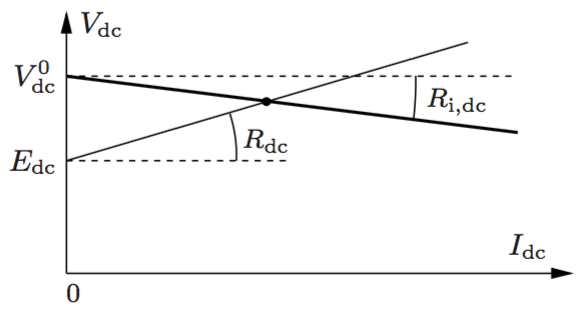
\includegraphics[scale=0.4]{ch2/7}
			\captionof{figure}{}
			\label{fig:2.6}
			\end{wrapfigure} 			
			
			If we take into account the voltage drop in the diodes, we have: 
 			\begin{equation}
 				V_{dc} = \underbrace{0.45 V_{ac} - V_{D,on}}_{V_{dc}^0} - \underbrace{(R_{D,on}+\frac{\omega L_{ac}}{2\pi})}_{R_{i,dc}} I_{dc}
			\end{equation} 	
			where the elements of the equation are gathered to form the Thevenin equivalent of the AC source and both diodes (non-ideal diodes with $V_{dc}^0$ and inner resistance $R_{i,dc}$). In \autoref{fig:2.6}, we can find the duty point. There are no Joule losses associated to $R_{i,dc}$. 
			
		\subsubsection{Non infinitely inductive load}
		
            For a non-ideal case, that is to say a real load and a real inductance $L_{dc}$, we can distinguish two cases. Continuous conduction, which results in an always positive distorted current $i_{dc}$. And the case where the current is discontinuous $i_{dc} = 0$ during some time intervals. When there is  \textbf{continuous conduction}, the equations of $\theta _{com}$ and $\Delta V_{com}$ remain good approximations. However, when we have \textbf{discontinuous conduction}, these equations are not valid and the commutation from $D1$ to $D2$ doesn't exist anymore. 
			
\section{Single-phase and three-phase bridges - basic formulas for the average output voltage}
	\begin{wrapfigure}[7]{l}{7.5cm}
	\vspace{-5mm}
	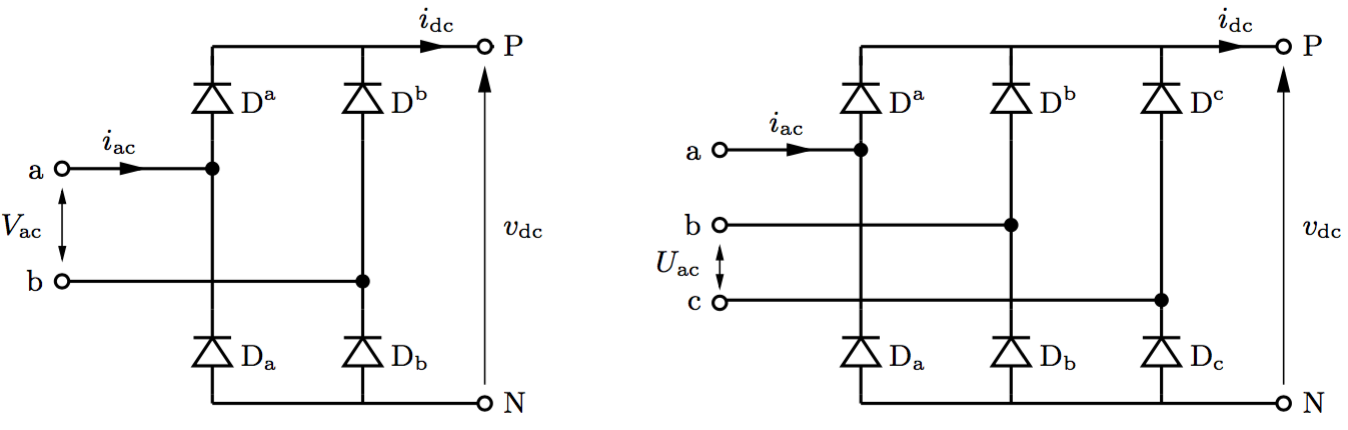
\includegraphics[scale=0.3]{ch2/8}
	\captionof{figure}{}
	\end{wrapfigure} 
	This figure represents a single-phase (where the input is an rms voltage $V_{ac}$) and a three-phase bridge (where the input is a phase-to-phase rms voltage $U_{ac}$). These bridges receive an AC voltage of frequency $f$ as an input. The output terminals furnish a DC voltage to a load. They are referred to as $P$ and $N$ and they are connected to the positive bus and the negative bus respectively. The instantaneous output voltage $v_{PN}(t)$ will be referred to as $v_{dc}(t)$. As both the positive and the negative alternations are employed these bridges are considered \textbf{full-wave rectifiers}. The input terminals are linked to the wire between two diodes. In the bridges the upper diodes ($D^i$) will work as maximum voltage selectors and the lower diodes ($D_i$) will work as minimum voltage selectors. This way, the instantaneous output voltage $v_{PN} \equiv v_{dc}$ is the maximum voltage amongst the input lines: 
	\begin{equation}
	\begin{aligned}
		single-phase &: v_{dc}(t) = \max (v_{ac}, -v_{ac}) = |v_{ac}|,\\
		three-phase &: v_{dc}(t) = \max (u_{ab}, -u_{ab}, u_{bc}, -u_{bc}, u_{ca}, -u_{ca})
	\end{aligned}
	\end{equation}
	
	\begin{wrapfigure}[10]{r}{4.2cm}
	\vspace{-5mm}
	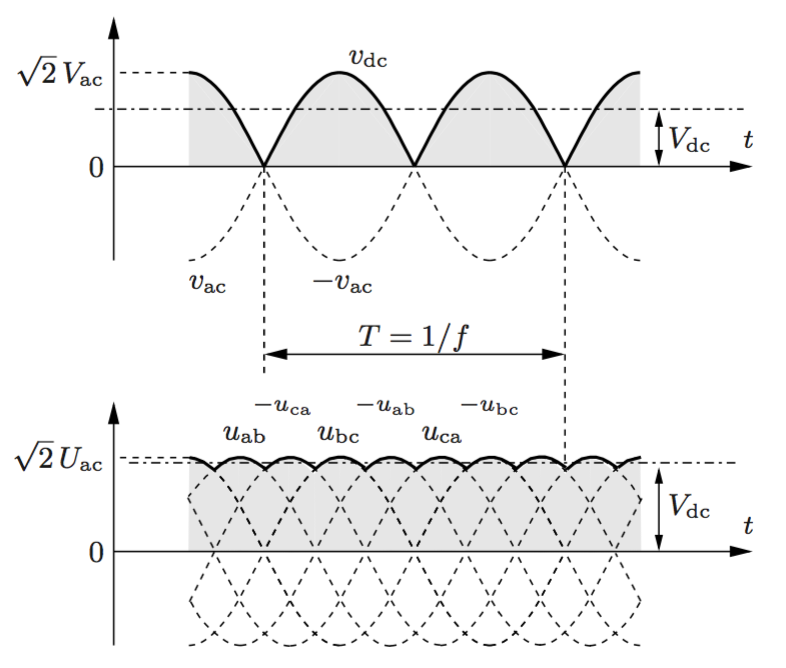
\includegraphics[scale=0.3]{ch2/9}
	\captionof{figure}{}
	\end{wrapfigure} 			
	This is easier to see graphically. We will only consider the upper envelope of the voltages as shown in the previous figure. We call it 2-pulse or 6-pulse rectification, which implies $2kf$ and $6kf$ harmonics in the spectres of the DC quantities.
	
	The output voltage of the three-phase bridge will be way less distorted ans it will fluctuate between $\sqrt{3/4}Û_{ac} = 0.866 Û_{ac}$ and $Û_{ac}$. Their average output voltages will be:
	\begin{equation}
		\begin{aligned}
		single-phase &: V_{dc} = \frac{1}{\pi}\int _{-\frac{\pi}{2}} ^ {\frac{\pi}{2}} \sqrt{2} V_{ac} \cos \omega t \, d\omega t = \frac{2\sqrt{2}}{\pi} V_{ac},\\
		three-phase &: V_{dc} = \frac{3}{\pi}\int _{-\frac{\pi}{6}} ^ {\frac{\pi}{6}} \sqrt{2} U_{ac} \cos \omega t \, d\omega t = \frac{3\sqrt{2}}{\pi} U_{ac},
		\end{aligned}
		\label{eq:2.14}
	\end{equation}
	The hypothesis needed to reach those values and conclusions were: 
	\begin{itemize}
		\item[•] The AC voltage source is ideal, $L_{ac} = 0$ (in practice $L_{ac}\neq 0$). 
		\item[•] Continuous conduction. In fact, we might have intervals during which any of the diodes conducts, when that happens $v_{dc}$ will only depend on the load. 
		\item[•] Ideal diodes (ideal characteristic). 
	\end{itemize}
	
\section{Bridges - operation with an inductive load (continuous conduction)}
	\subsection{Single-phase bridge and infinitely inductive load}
		\begin{wrapfigure}[4]{l}{4.5cm}
		\vspace{-5mm}
		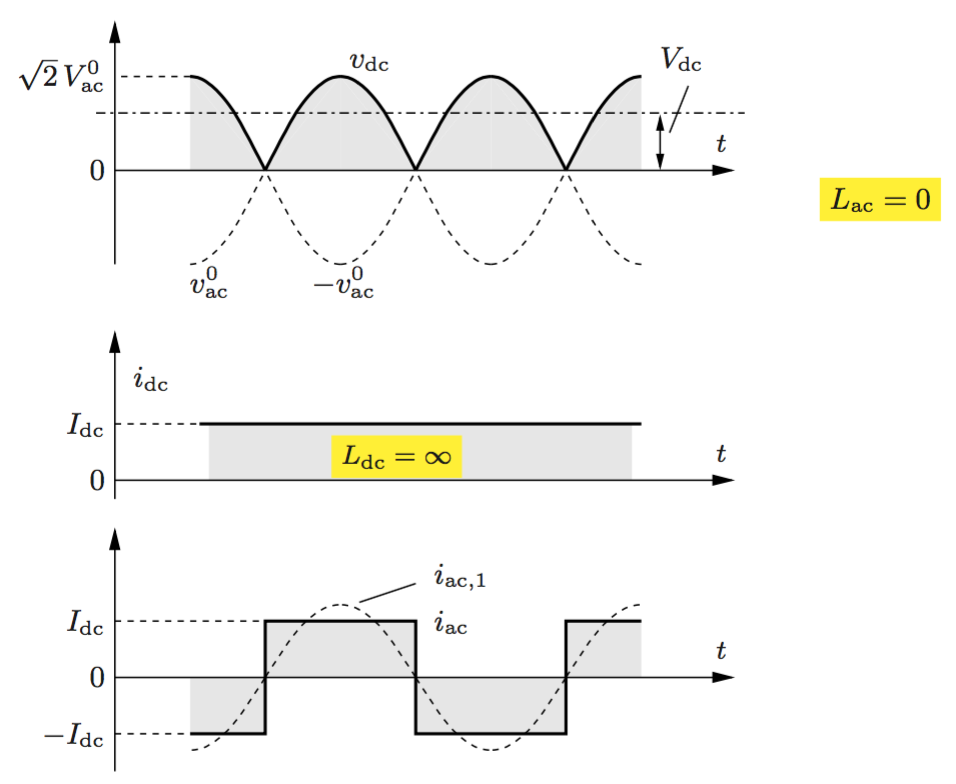
\includegraphics[scale=0.25]{ch2/10}
		\captionof{figure}{}
		\end{wrapfigure} 
		First, we consider an ideal AC load $L_{ac} = 0$ and a DC RLE load with $L_{dc}\rightarrow \infty$. During positive alternations of the input voltage $v_{ac}^0$, diodes $D^a$ and $D_b$ are conducting and during negative alternations diodes $D^b$ and $D_a$ will conduct. The smooth DC output current $i_{dc}$ implies a square-wave input current. The fact that $L_{ac} = 0$ allows the discontinuity of the current during commutations. The amplitude of the fundamental input current is $I_{ac,1} = \frac{2\sqrt{2}}{\pi} I_{dc}$. It is in phase with $v_{ac}^0$ and, consequently, $DPF = \cos \varphi _1 \approx 1$. That is the case of almost every diode rectifier. However, the $PF<1$ because of the distortion of the square-wave current. We can check the power balance with the equation \eqref{eq:2.14} : 
		\begin{equation}
			V_{ac}^0I_{ac,1} \cos \varphi _1 = V_{dc} I_{dc}.
		\end{equation}
		When $L_{dc} \neq \infty$, the current is not constant and it fluctuates with $I_{dc,min} \geq 0$. When $E_{dc}<V_{dc}$, the current will be continuous as long as $L_{dc}$ remains big enough. In this case, we have discontinuous conduction and \eqref{eq:2.14} is still valid. Taking into account the voltage drop in the diodes, we can increase the accuracy of this equation: 
		\begin{equation}
			V_{dc} = 0.9003 V_{ac}^0 - 2 V_{D,on} - 2 R_{D,on} I_{dc}
		\end{equation}
		
	\subsection{Three-phase bridges and infinitely inductive load}
		\begin{wrapfigure}[13]{l}{5.6cm}
		\vspace{-5mm}
		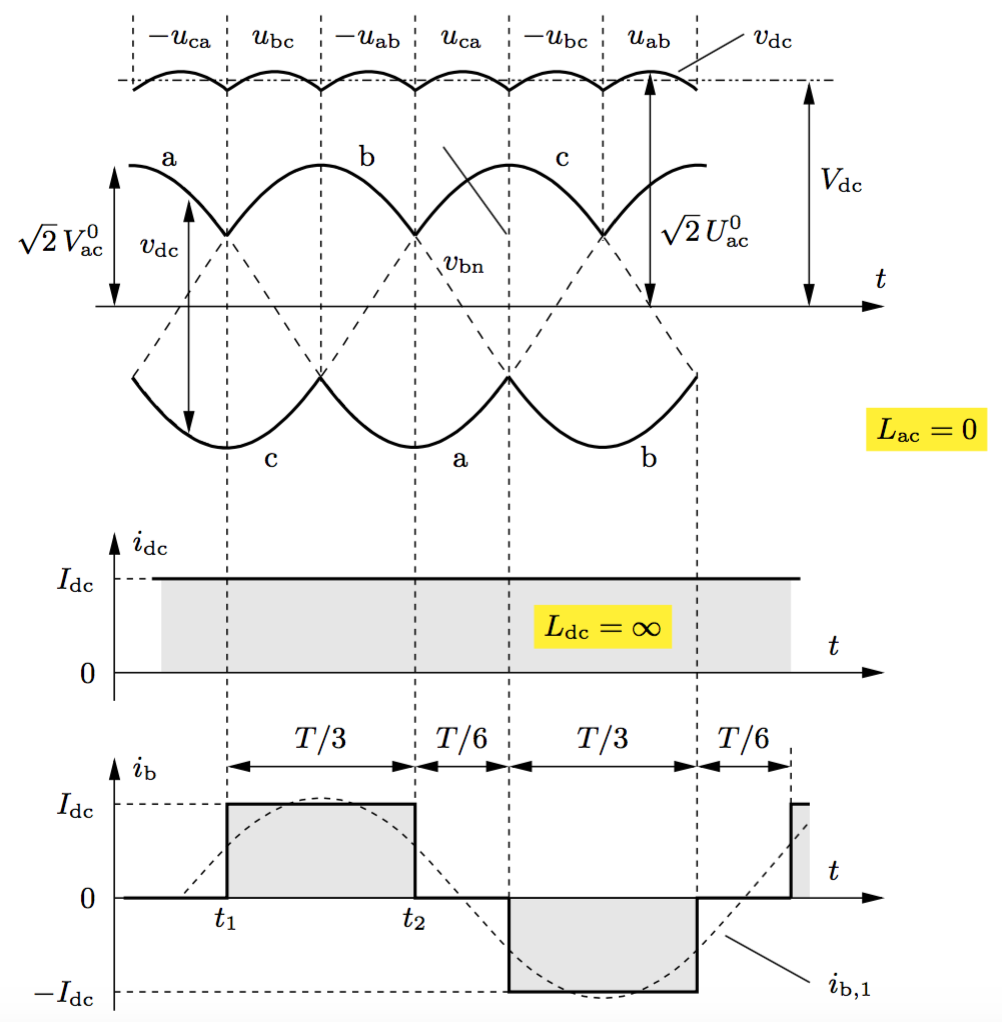
\includegraphics[scale=0.3]{ch2/11}
		\captionof{figure}{}
		\end{wrapfigure} 
		They operate following the same principle as the single-phase bridge. However, here each phase conducts during 2 times 120$^\circ$.\\
		The ideal voltage source is represented by its star connected equivalent circuit. We will consider $L_{dc} = \infty$ and the 3 phases will contribute symmetrically to the constant DC current. During a fundamental period, each phase will conduct for 2 times 120$^\circ$  and will block the current during 2 times 60$^\circ$. The 3 currents constitute a three-phase square wave. Once again, the fundamentals of the currents are in-phase with their respective voltages and $\varphi _1 = 0 \Rightarrow \cos \varphi _1 = 1$. The rms value of the fundamental component of the current is $I_{ac,1} = \frac{\sqrt{6}}{\pi}I_{dc}$. This way the power balance is:

		\begin{equation}
			\sqrt{2}V_{ac}I_{ac,1} \cos \varphi _1= V_{dc}I_{dc}. 
		\end{equation}
		
		In the \textbf{continuous} case, \eqref{eq:2.14} remains valid as long as we add the losses inside the 2 conducting diodes. 
		
	\subsection{Single-phase bridges, commutation between diodes}
	    
	    In a system we might have, besides the inner inductance of the source, a smoothing inductance or an LC filter after the diodes. When that happens the commutation cannot be immediate anymore. \\
		
	\begin{wrapfigure}[8]{r}{5cm}
		\vspace{-5mm}
		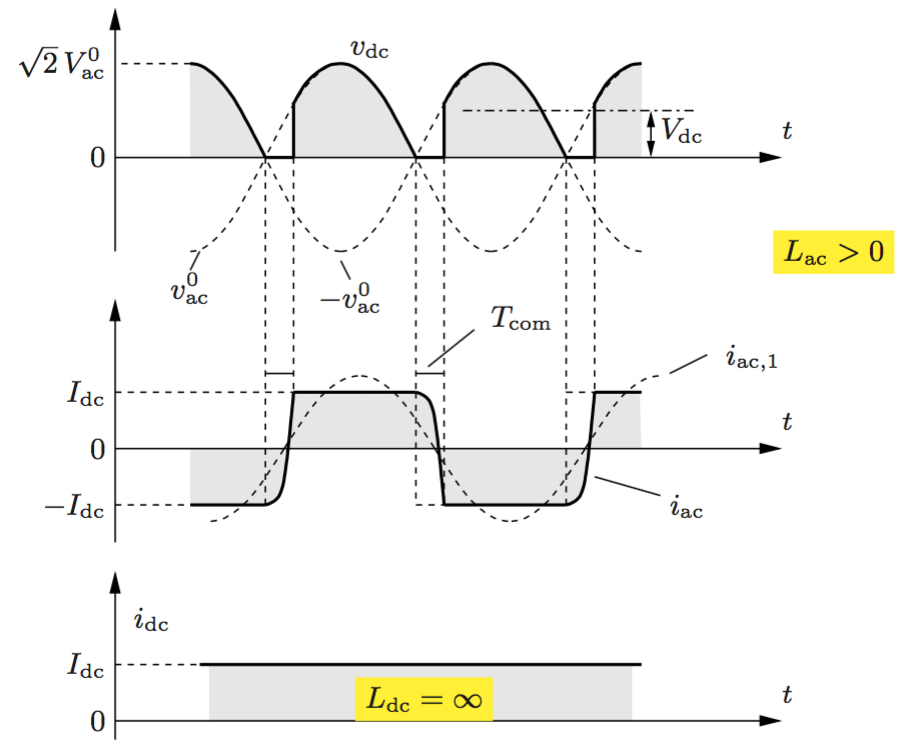
\includegraphics[scale=0.3]{ch2/12}
		\captionof{figure}{}
		\end{wrapfigure} 
		First we will study a circuit with an inductance before the rectifier $L_{ac} \neq 0$. The figure represents the commutation intervals $T_{com}$. We can demonstrate that with an infinitely inductive load the output voltage will be the average of those appearing during the commutation, thus nil. So the commutation will take: 
		\begin{equation}
			\omega T_{com} = \arccos \left( 1-\frac{2\omega L_{ac}}{\sqrt{2}V_{ac}^0} I_{dc}\right). 
		\end{equation}
		
		We can now calculate the drop of the average DC voltage: 
		\begin{equation}
			\Delta V_{dc} = \frac{2\omega L_{ac}}{\pi}I_{dc}. 
		\end{equation}
		
		\begin{wrapfigure}[5]{l}{4cm}
		\vspace{-5mm}
		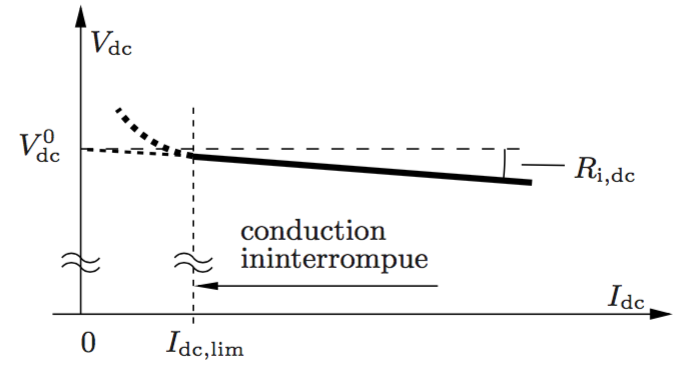
\includegraphics[scale=0.3]{ch2/13}
		\captionof{figure}{}
		\end{wrapfigure} 
		We can therefore express the average voltage with the voltage drops in the diodes and $\Delta V_{dc}$ then group together the DC voltage source with its inner resistance (Thevenin) : 
		\begin{equation}
			V_{dc} = \underbrace{0.9003 V_{ac}^0 - 2V_{D,on}}_{V_{dc}^0} - \underbrace{\left( 2 R_{D,on} + \frac{2\omega L_{ac}}{\pi} \right)}_{R_{i,dc}} I_{dc}
		\end{equation}
		This characterization of average values is only valid when conduction is continuous. It will become discontinuous when the current goes over a certain limit value called $I_{dc,lim}$. Because of the overlapping, the fundamental component of the current has a lag with respect to the voltage $v_{ac}^0$ with $\varphi _1 >0$ and $DF = \cos \varphi _1 < 1$. \\
		
		With a three-phase system, the obtained equations are: 
		\begin{equation}
			\omega T_{com} = \arccos \left( 1-\frac{2\omega L_{ac}}{\sqrt{2}U_{ac}^0} I_{dc}\right) \qquad \Delta V_{com} = \frac{3\omega L_{ac}}{\pi} I_{dc}.
		\end{equation}
		
\section{Diode bridges - operation with smoothing of the DC voltage (by a capacitor)}
    We will connect the capacity $C$ in parallel with the load in order to smooth the voltage. The distortion of $v_{dc}(t)$ will become smaller as we put bigger capacities. If the capacity is infinitely big the voltage will be perfectly smooth $V_{dc}$, but there are disadvantages to this solution: the energy and time needed to charge the capacity will also be infinite. For the moment, the load considered will only consist of a resistance $R_{dc}$. The voltage $v_{dc}(t) = v_C(t)$ will be linked to the current by the equation:
	\begin{equation}
		C\frac{dv}{dt} = i_C = i_{dc} - i_{dc,R}
	\end{equation}
	where $i_{dc}$ and $i_{dc,R} > 0$. At steady state, the rms value of the current flowing through the capacity $I_C = 0$. The DC current becomes $I_{dc} = I_{dc,R}$ and as Joules' law implies, it will be higher for smaller resistances. When there is no load, the open circuit will work as an infinite resistance $R_{dc}=\infty$ and thus there will be no conduction.
	
	\subsection{Single phase diode bridges with smoothing of the output voltage}
		\begin{wrapfigure}[7]{r}{7.5cm}
		\vspace{-5mm}
		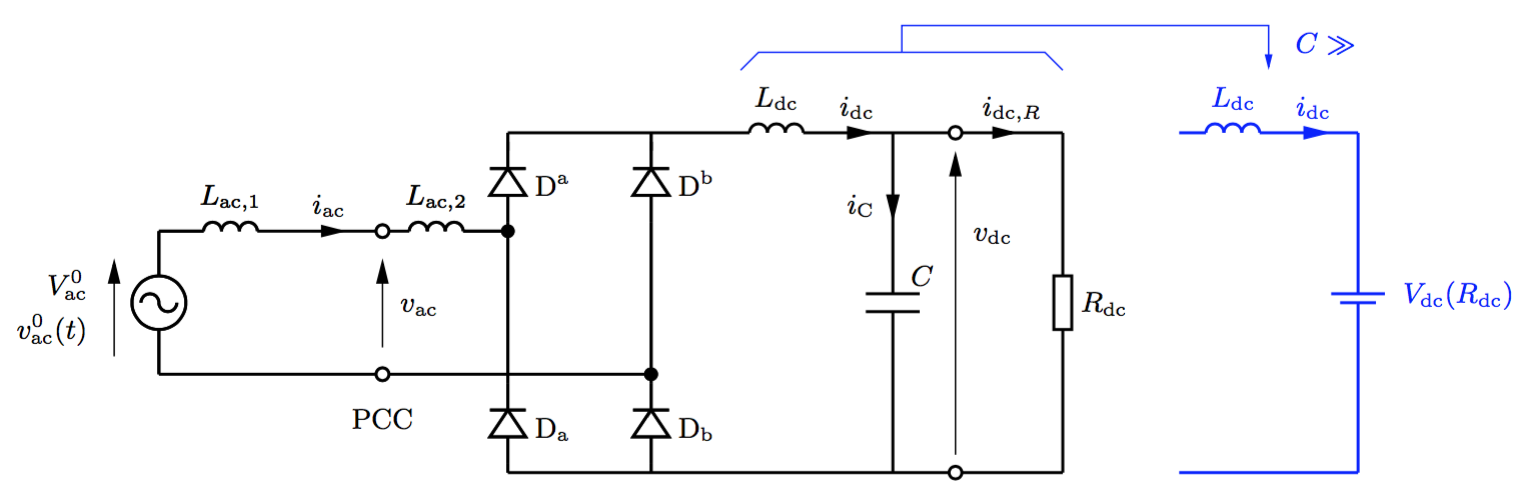
\includegraphics[scale=0.27]{ch2/14}
		\captionof{figure}{}
		\end{wrapfigure} 
		This circuit has three inductances, one corresponds to the inner impedance of the source $L_{ac,1}$, another one to the smoothing inductor at the input $L_{ac,2}$ and the last one to a second smoothing self $L_{dc}$. The inductors considered here are perfect, that is to say without inner resistance. Other loads can be connected to the source via the PCC, where the voltage is:
		
		\begin{equation}
			v_{ac}(t) = v_{ac}^0(t) - L_{ac,1}\frac{di_{ac}}{dt}.
		\end{equation}
		
		If we consider that $v_{ac}^0$ is perfectly sinusoidal (the only component is the fundamental harmonic), the only distortion is generated by the current $i_{ac}$. If we write the harmonic components of the voltage $v_{ac}^0(t)$ as a function of the rms values of harmonics of order $k>1$ of the current $i_{ac}(t)$:
		
		\begin{equation}
			v_{ac,k}(t) = -L_{ac,1}\frac{di_{ac,k}}{dt} \qquad \Rightarrow  V_{ac,k} = k\omega L_{ac,1} I_{ac,k}.
		\end{equation}
	    It is easy to see the interest of limiting the distortion of the current if we want to limit the distortion of the voltage. Thanks to the capacitor the output voltage will be barely distorted. We can model that RC load as an ideal DC voltage source whose value $V_{dc}=cst$ will be function of $R$. 
		
		\subsubsection{Discontinuous conduction}
			\begin{wrapfigure}[9]{l}{6cm}
			\vspace{-5mm}
			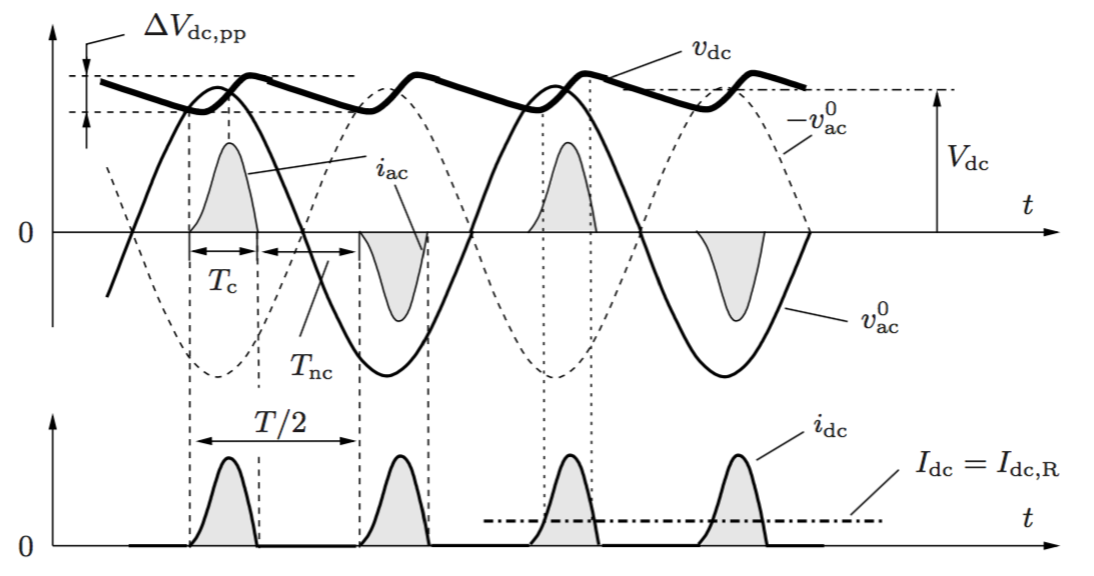
\includegraphics[scale=0.3]{ch2/15}
			\captionof{figure}{}
			\end{wrapfigure} 
			In this figure we can see the distortion of the output voltage. As there are intervals $T_{nc}$ during which $i_{ac} = 0$, conduction is discontinuous. These intervals are delimited by current impulsions that last $T_{c}$, with:
			\begin{equation}
				T_{nc} + T_c = \frac{T}{2}.
			\end{equation}
			
		    Conduction takes place by diode couple, without overlapping (4 diodes conducting simultaneously). The rectified current $i_{dc} = |i_{ac}|$ possesses 2 positive impulsions by fundamental period. The current $i_{ac} \neq 0$ only flows when $|v_{ac}^0(t)| \geq v_{dc}(t)$. Thanks to the total inductance $L_{ac} + L_{dc}$, the current $i_{ac}$ grows until it reaches its maximum when $|v_{ac}^0| = v_{dc}$. Conduction will last until the energy stored in the inductances runs out. During these conduction intervals $T_c$, the differential equations of the rise and the descent of $i_{dc}$ is:
			\begin{equation}
				(L_{ac}+L_{dc})\frac{d_{i_{dc}}}{dt} = |v_{ac}(t)|-v_{dc}(t).
			\end{equation}
			
			\textbf{Output voltage} \qquad In a real case, where $C$ is finite, $v_{dc}(t)$ has \textit{sawtooth} shape. The fluctuation will be lesser for higher capacities. During $T_{nc}$ (when $i_{dc} =i_{ac} =0$), the load and the capacitor are not fed by the source. Instead, the capacitor will use its stored energy to feed the load. If the time constant of the circuit $\tau = R_{dc}C$ is big with respect to $T/2$, the falling edges of the fluctuation are almost straight lines with a gradient $-V_{dc}/\tau$ : 
			\begin{equation}
				C\frac{v_{dc}(t)}{dt} = -i_{dc,R}(t) = \frac{v_{dc}(t)}{R} \qquad \Rightarrow \qquad \frac{dv_{dc}}{dt} \approx - \frac{V_{dc}}{R_{dc}C} \qquad (i_{dc} = 0).
			\end{equation}
			
			During a conduction interval $T_c$, $v_{dc} = v_c$ reaches a maximum value when $i_{dc} = i_{dc,R}$ as depicted in (Eq.:2.22)\eqref{eq:2.22}. The minimum output voltage will appear at the beginning of $T_c$ and the maximum at the end. The peak-to-peak ripple $v_{dc}(t)$ will be approximated as follows:
			\begin{equation}
				\Delta V_{dc,pp} \approx \frac{T_{nc}}{R_{dc}C}V_{dc},
			\end{equation}
			Its upper limit is obtained when $T_{nc} = T/2$.
			\\
			
			\textbf{Output current} \qquad As $v_{dc}$ is little distorted, the current $i_{dc} = v_{dc}/R_{dc}$ will be little distorted too. The current in the capacitor $i_c = i_{dc}-i_{dc,R}$ is the difference between $i_{dc}$ in thin impulsions $\pm$ and $i_{dc,R}$ is quasi constant. Remember: $i_c$ is an AC current with a nil average value at steady state. 
			\\
			
			\textbf{Dimensionless output voltage/current characteristics} \qquad We will focus on the global characteristic of the output, the average output voltage $V_{dc}$ versus the average output current $I_{dc}$ that is to say the load resistance $R_{dc}=V_{dc}/I_{dc}$, while considering a capacity big enough to neglect its effect on the characteristic. The remaining parameters are 

			\begin{wrapfigure}[8]{r}{6cm}
			\vspace{-5mm}
			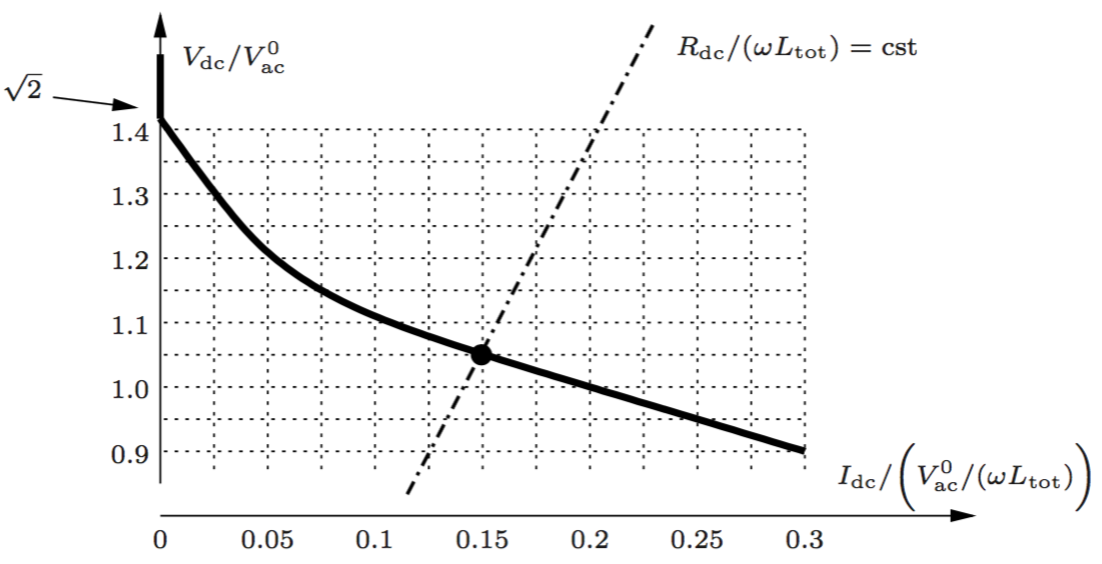
\includegraphics[scale=0.3]{ch2/16}
			\captionof{figure}{}
			\end{wrapfigure} 
			thus $V_{ac}^0, \omega$ and $L_{tot}$ (for the discontinuous case). We will render $V_{dc}$ and $I_{dc}$ dimensionless by dividing them by $V_{ref} = V_{ac}^0$ and $I_{ref} = V_{ac}^0/(\omega L_{tot})$. We can now represent the characteristic of the output with a single curve as in the figure. This curve won't change if we modify the values $V_{ac}^0, \omega$ and $L_{tot}$ as long as $C$ is big. We see that $V_{dc}$ grows closer to 
			$\sqrt{2}V_{ac}^0$ as the load diminishes ($R_{dc}$ growing, $I_{dc}$ shrinking). When we lack a load ($R_{dc} = \infty$, $I_{dc} = 0$), the capacitor remains charged at a voltage of at least $\sqrt{2}V_{ac}^0$ and current doesn't flow in the diode bridge. \\
			When the load increases ($R_{dc}$ shrinks), we go down the curve, $V_{dc}$ drops and $I_{dc}$ increases. That happens at the same time as the commutation intervals $T_c$ grow longer. Lastly we get to the limit betwee continuous and discontinuous conductino, where $T_c = T/2$ and the current impulsions merge. Trough numeric simulation we observe this limit at $I_{dc} \approx 0.3 V_{ac}^0/(\omega L_{tot})$, which corresponds to the point {0.3, 0.9} of the curve. The THD of $i_{ac}(t)$ growss bigger with minor loads. On the other hand, the lag of the fundamental component of $i_{ac}(t)$ with respect to $v_{ac}(t)$ is low, which gives a $DPF = \cos \varphi _1 \approx 1$. 
			
		\subsubsection{Discontinuous conduction}
			\begin{wrapfigure}[8]{l}{6cm}
			\vspace{-5mm}
			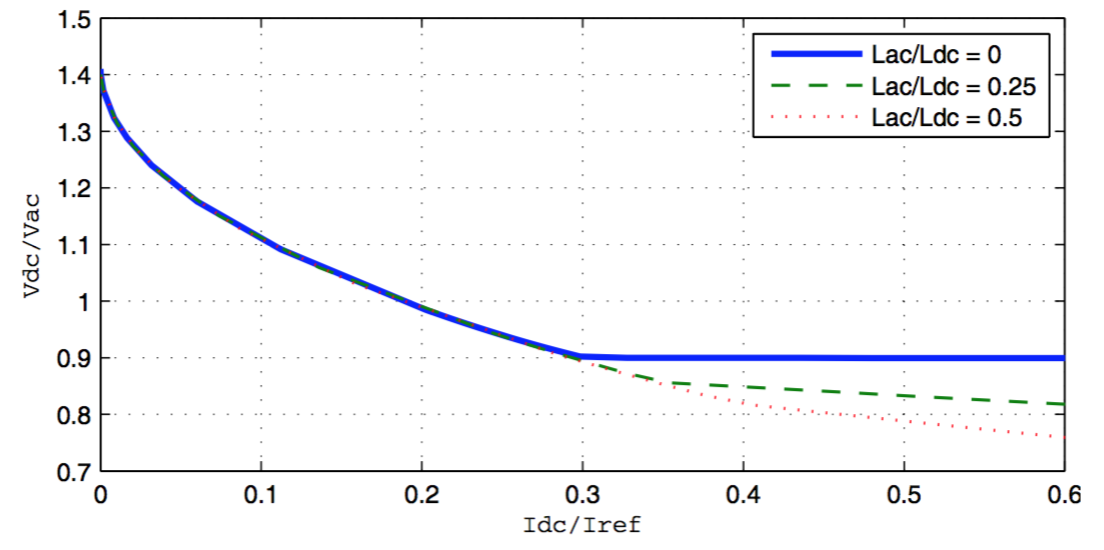
\includegraphics[scale=0.3]{ch2/17}
			\captionof{figure}{}
			\end{wrapfigure} 
			
			In this case, when $I_{dc}/I_{ref}>0.3$ the carried study becomes pertinent once again. The voltage $v_{dc}$ mainly constant thanks to the capacitor corresponds to an $E_{dc}$ of the load. $L_{dc}$ corresponds to the inner inductance of the load and it has little effect on the voltage. However, $L_{ac}$ is the cause of the encroachment that nullifies the output voltage. Through 3 simulations with different values of $L_{ac}$ and $L_{dc}$ while keeping the same $L_{tot}$, a variable $R_{dc}$ for each arrangement and a big constant capacity, we get these three curves. When $0<I_{dc}/I_{ref}<0.3$ conduction is continuous and the curves follow the same pattern. This shows that $L_{tot}$ is the inductance that will impose the characteristic of the system and not a single inductance by herself. For greater dimensionless currents, the dimensionless voltage will decrease linearly with the current because of the encroachment caused by $L_{ac}$.
			
	\subsection{Three-phase diode bridges}
	
		\begin{center}
		\begin{minipage}{0.45\textwidth}
			\begin{flushleft}
			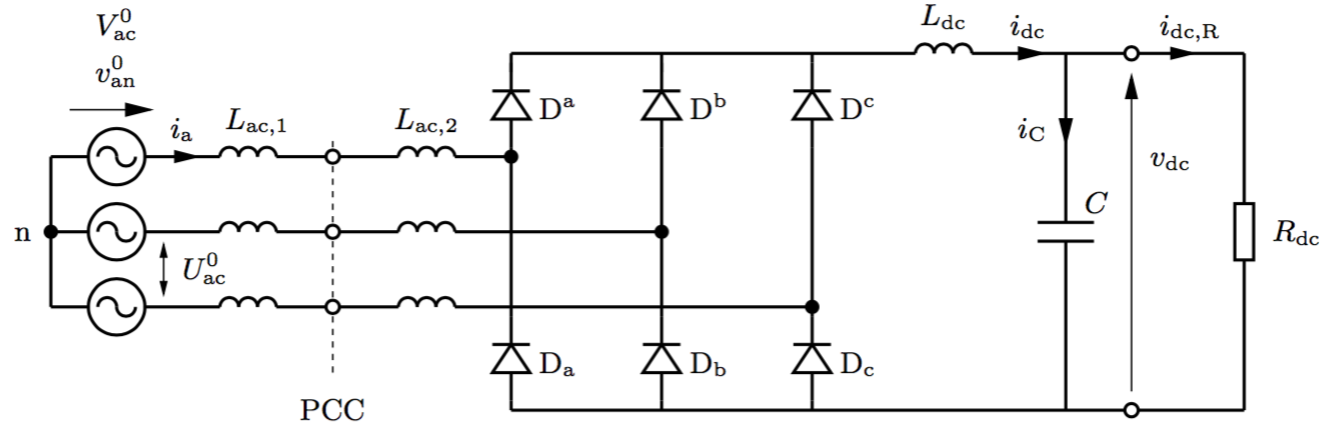
\includegraphics[scale=0.3]{ch2/18}
			\captionof{figure}{}
			\end{flushleft}
		\end{minipage}			
		\begin{minipage}{0.45\textwidth}
			\begin{flushright}
			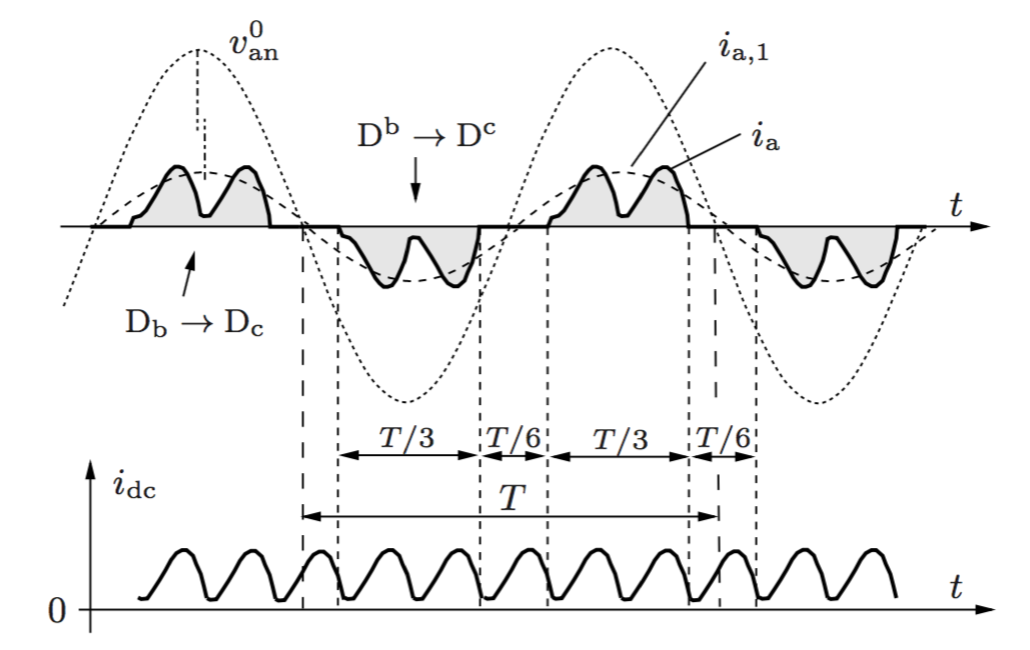
\includegraphics[scale=0.35]{ch2/19}
			\captionof{figure}{}
			\end{flushright}
		\end{minipage}			
		\end{center}
		
		This is the equivalent circuit of the three-phase system. In this figure each input line comprises the inductances $L_{ac,1}$ and $L_{ac,2}$ but there is a single $L_{dc}$ set after the rectifier. The classical shape of the AC current furnished by the source is also represented. When the current is continuous each phase current flows during 2 conduction intervals of 120$^\circ$. The depression between the conduction intervals of a single phase corresponds to the commutation between the two remaining phases as pointed in the figure.\\
		
		\textbf{Discontinuous conduction}\qquad When the load diminishes ($R_{dc}$ increases) and the conduction becomes discontinuous, the AC current contains 2 positive impulsions separated by an interval of non-conduction by fundamental period of the AC source. Each fundamental period also contains two negative impulsions showing the same phenomena as the positive ones. We have $i_{dc} = |i_{ac}|$ and during the conduction intervals the current flows through $L_{dc}$, two out of six diodes and two out of three input inductances $L_{ac}$. \\
		
		\begin{wrapfigure}[8]{l}{6cm}
		\vspace{-5mm}
		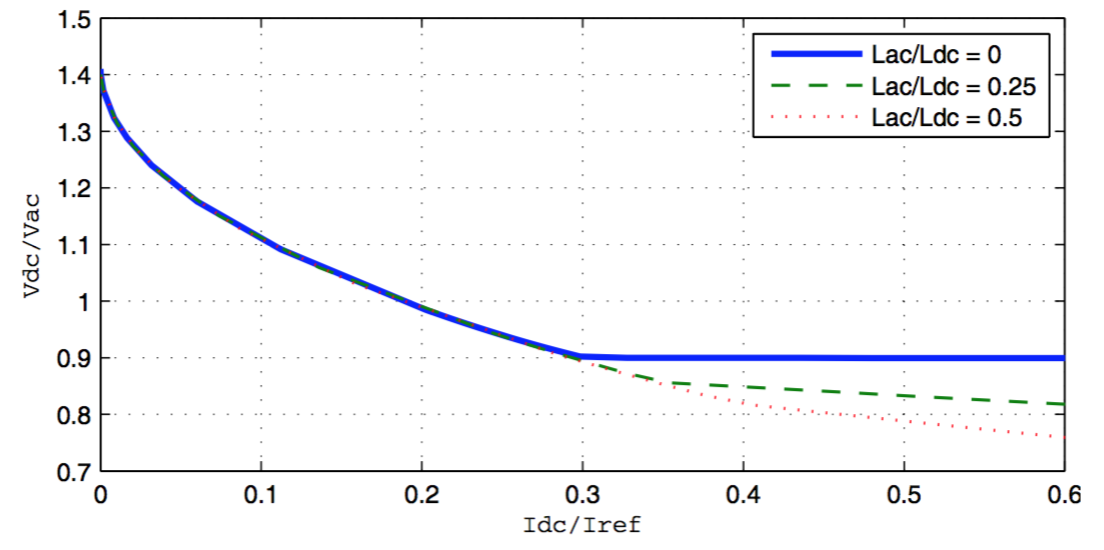
\includegraphics[scale=0.3]{ch2/17}
		\captionof{figure}{}
		\end{wrapfigure} 
		\textbf{Dimensionless output voltage/current characteristics}\qquad 		 We will choose as reference values $V_{ref} = U_{ac}^0$ and $I_{ref} = I_{ac}/(\omega L_{tot})$. This time it is appropriate to definite $L_{tot} = L_{dc}+ 2L_{ac}$. The simulation employed in the single-phase case is applied and the obtained curves appear in the graphic in the left. We remark the limit between discontinuous and continuous conduction at $I_{dc}/I_{ref} = 0.013$ and the ratio of 1.35 between $V_{dc}$ and $U_{ac}^0$ when conduction is discontinuous is easily observed. 
			
%%%%%%%
% Ch3       %
%%%%%%%

\chapter{Thyristor converters}
	In this chapter we will focus on rectifiers/inverters with thyristors and a controllable and invertible output. They are bridges obtained by replacing the diodes of the bridges studied in Chapter 2 by thyristors. We will also study \textbf{half-controlled bridges}. These half-controlled bridges are composed of diodes and thyristors. Consequently they are controllable but irreversible. Finally we will study AC choppers and cycloconverters, that will allow us to do AC/AC conversions without going through the DC. Choppers are composed of \textbf{triacs}, \textbf{bidirectional and semi-controllable switches}. 
	
	\section{Characteristics of thyristors}
		\begin{wrapfigure}[8]{l}{7cm}
		\vspace{-5mm}
		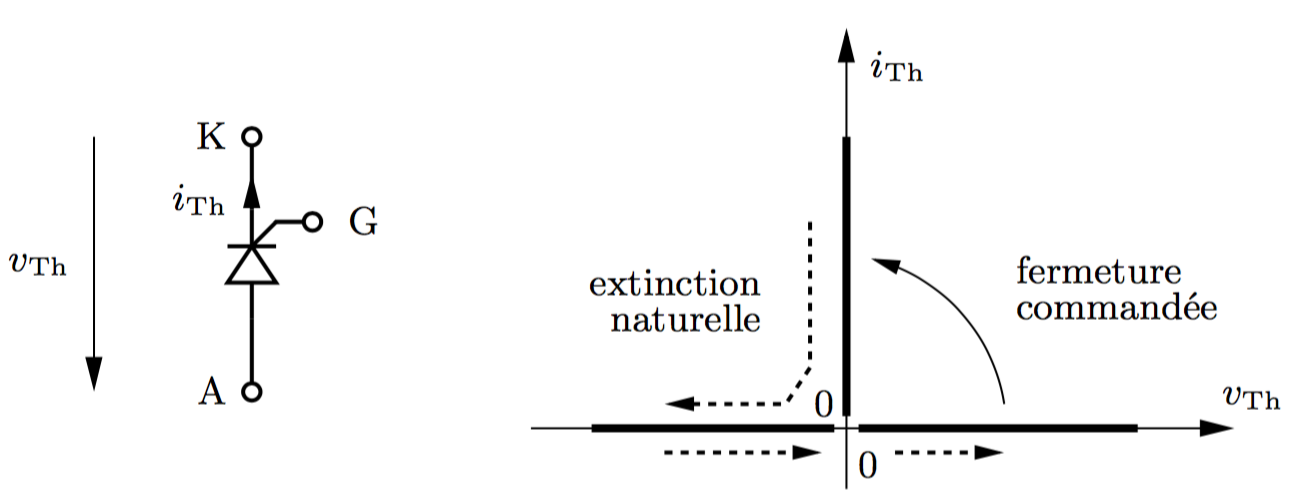
\includegraphics[scale=0.3]{ch3/1}
		\captionof{figure}{} 
		\label{fig:3.1}
		\end{wrapfigure}
		A thyristor (also called SCR: Silicon Controlled Rectifier) is represented in \autoref{fig:3.1}. During conduction the current $i_{Th} > 0$ flows from the anode A to the cathode K and the \textbf{gate G} allows us to choose the starting moment. It has the same behaviour as a diode. When it is \textbf{inversely biased} ($V_{AK}<0$), there is a leakage current $<0$ that can be neglected most of the times. When it is \textbf{directly biased}, it will only conduct when positive current impulsions go into the gate. As the diode does, the thyristor turns itself off when there is no current $i_{AK}$ going through it. That is why they are called \textbf{semi-controllable}. We can make them fully-controllable by adding an extra commutation circuit, which will increase the complexity of the device and will increase the losses. \\
		
		The direct and inverse voltage and the conduction current a thyristor can endure can go up to some \textbf{kilo} volts/amperes. The voltage drop due to conduction is of more or less 1 V and it is referred to using $V_{Th,on}$ and $R_{Th,on}$. The frequency capability is nevertheless very limited. In the case of the grid that is not a problem but it will be problematic when frequencies becomes greater than some hundreds of Hertz. 


	\section{Elementary circuits with one or two thyristors}
		\subsection{Circuit with one thyristor and a resistance}
		    When we have an ideal AC voltage source, the current $i_{ac}(t) = i_{dc}(t)$. During positive alternations, the thyristor is in direct-bias. The impulsions in the gate are given with a delay $\alpha$ [rad] called \textbf{firing angle} that ranges from 0 to $\pi$. When $v_{ac}$ becomes negative, $i_{dc}$ and $v_{dc}$ will become negative too and the thyristor will turn itself off (inverse-bias). That circumstance is represented in \autoref{fig:3.2}. The average value of the rectified voltage will be:
			\begin{equation}
				V_{dc} = \frac{1}{2\pi}\int _\alpha ^\pi \sqrt{2} V_{ac} \sin \omega t \, d\omega t = \frac{\sqrt{2}}{\pi} \frac{1+\cos \alpha}{2} V_{ac}.
			\end{equation}
			
			\begin{minipage}{0.49\textwidth}
				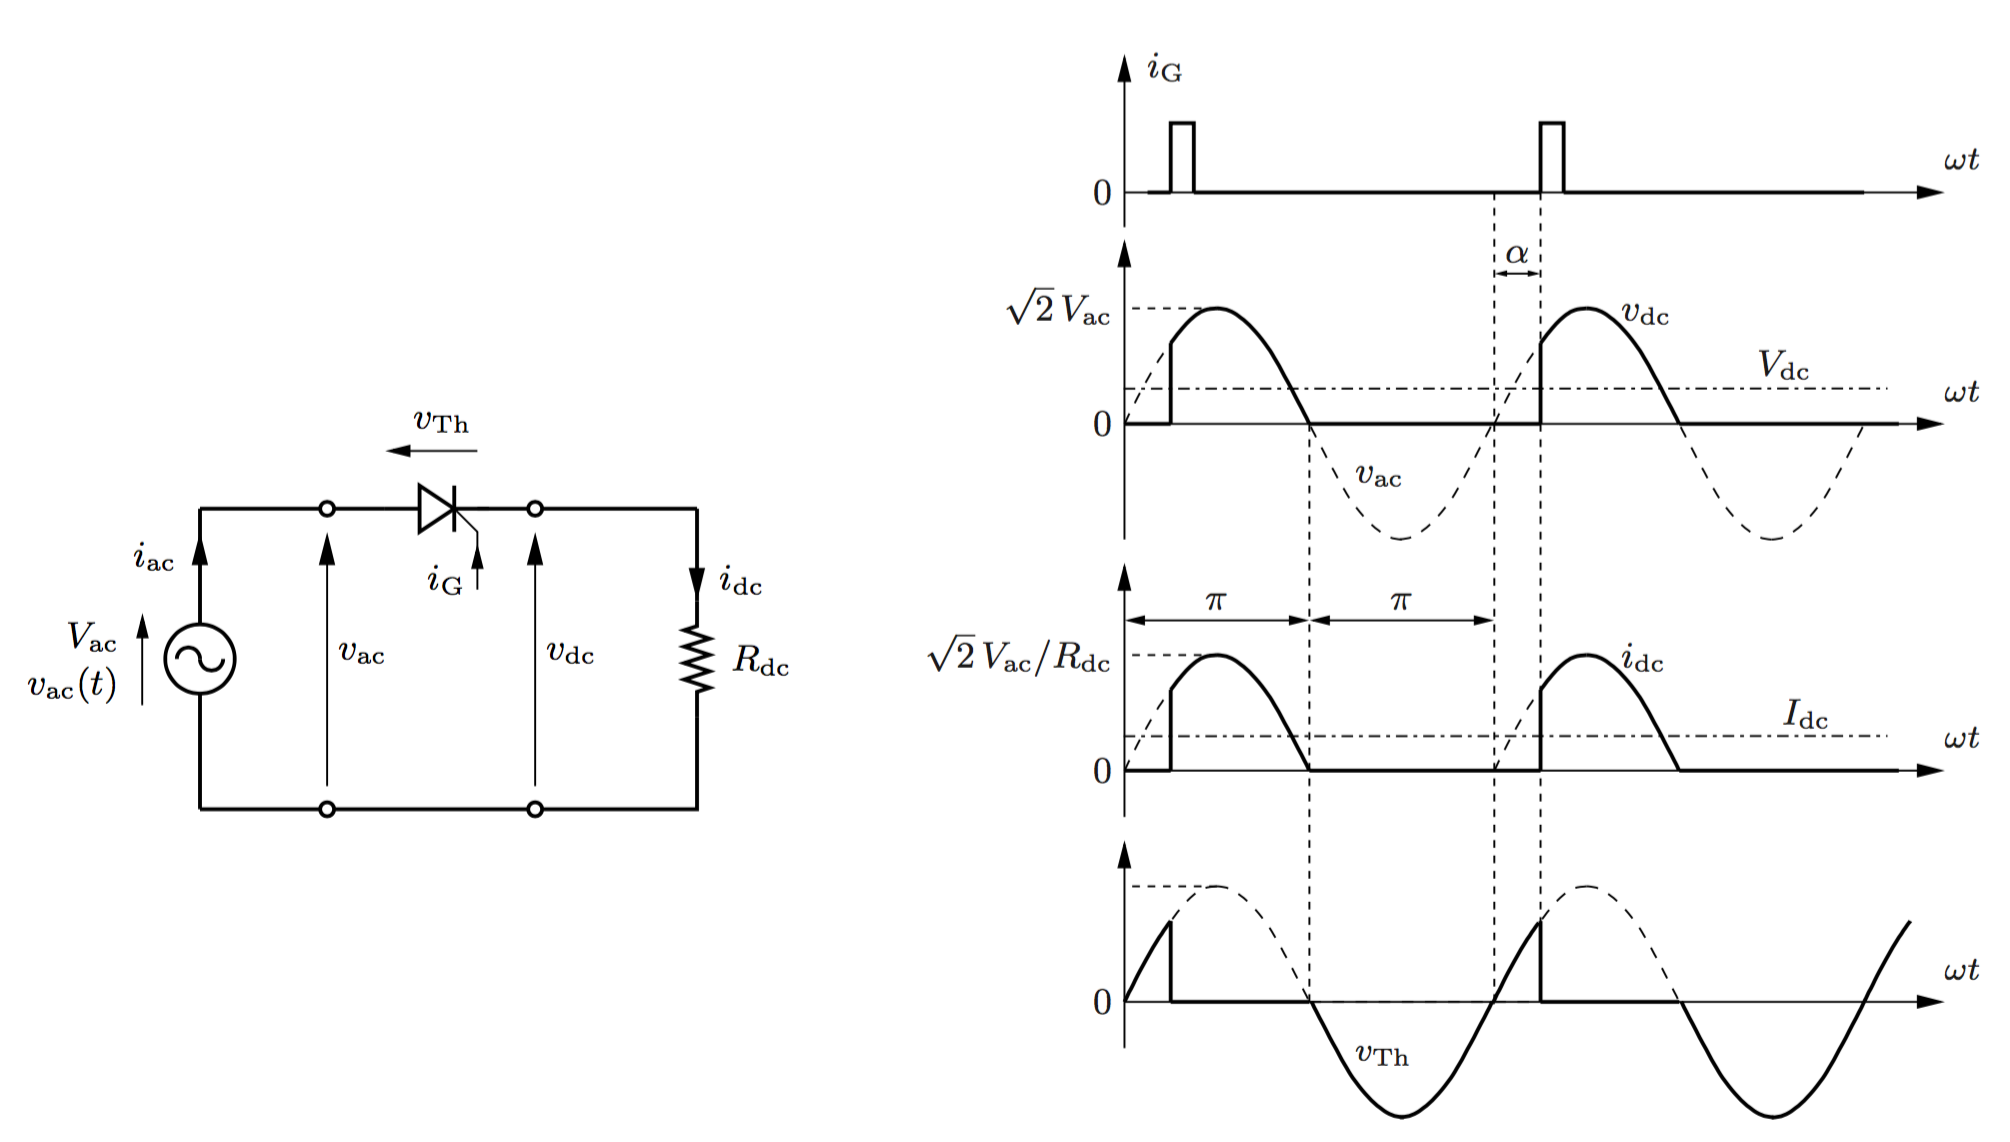
\includegraphics[scale=0.2]{ch3/2}
				\captionof{figure}{}
				\label{fig:3.2}
			\end{minipage}
			\begin{minipage}{0.49\textwidth}
				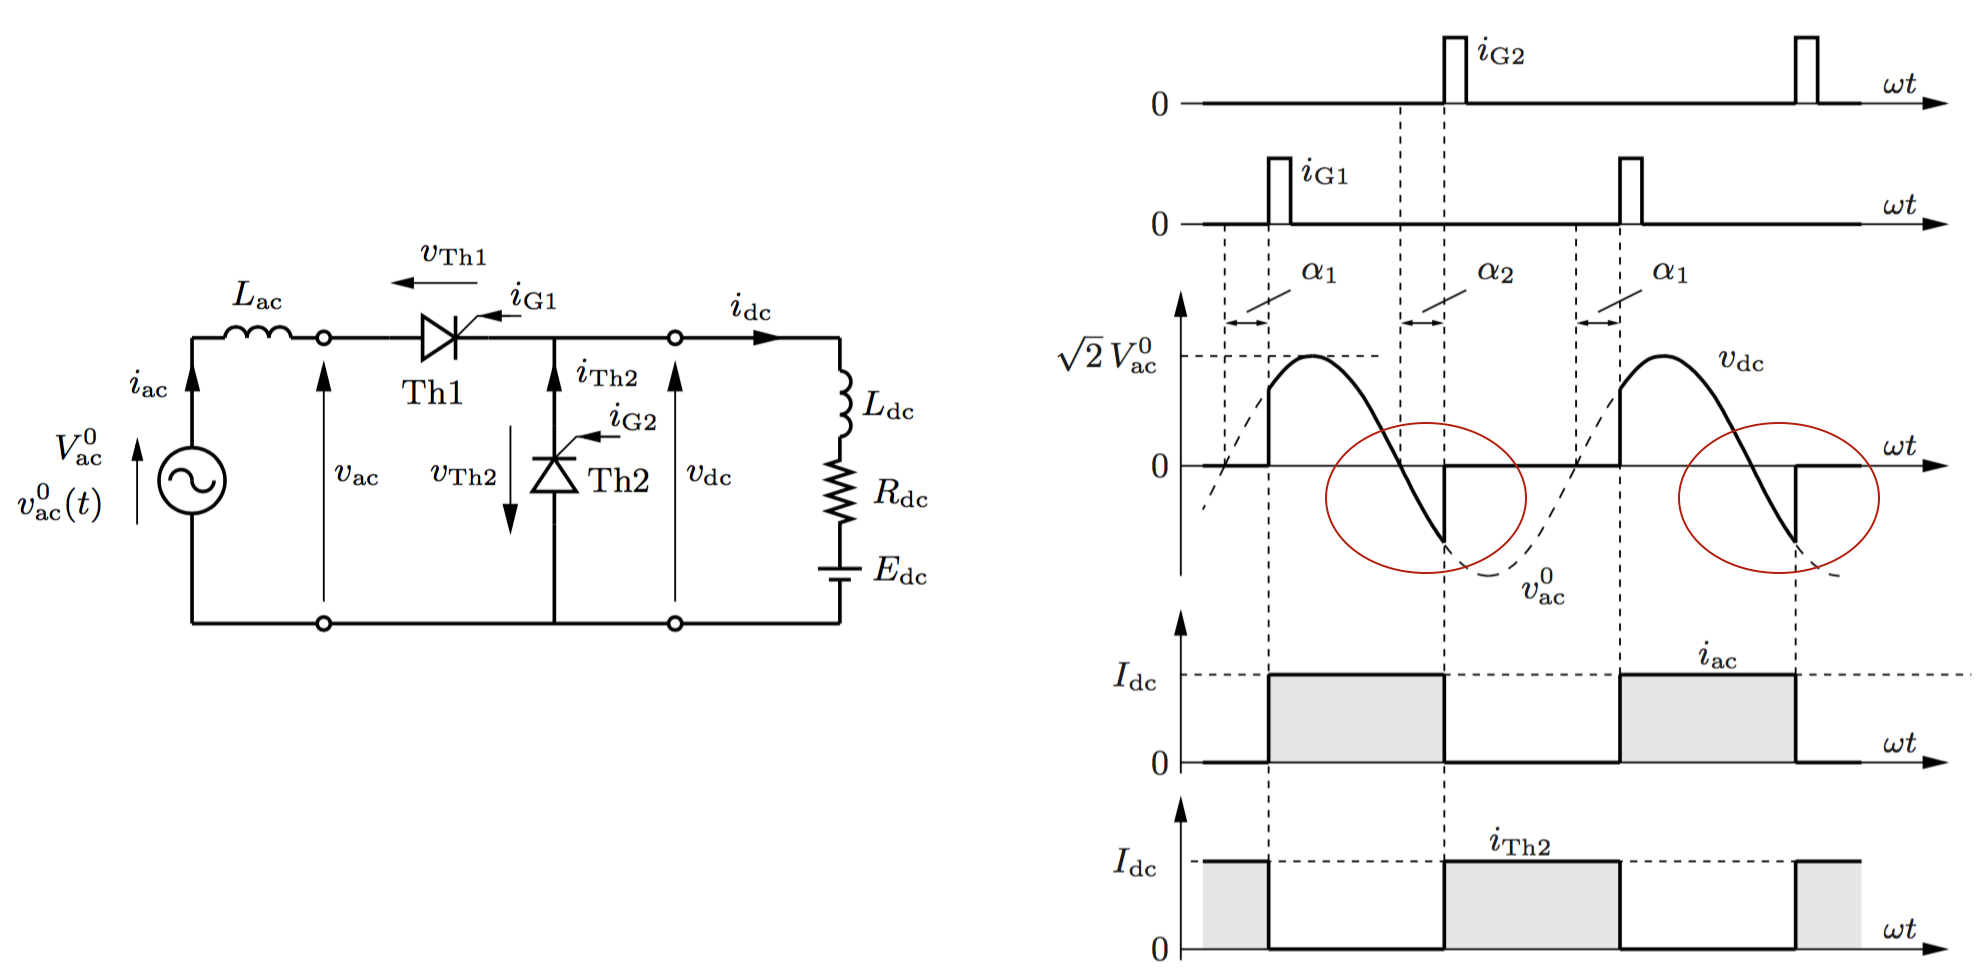
\includegraphics[scale=0.21]{ch3/3}
				\captionof{figure}{}
				\label{fig:3.3}
			\end{minipage}
			
		\subsection{Circuit with a rectifier thyristor and a free-wheeling thyristor}
		This distribution is shown in \autoref{fig:3.3}, where we can see 2 diodes Th1 and Th2. We will distinguish two different cases depending on the source.  
			
			\subsubsection{With ideal voltage source (without inductance)}
				The wave shapes when $L_{ac} = 0, L_{dc} = \infty$ are drawn in \autoref{fig:3.3}. We can see that the conduction interval of Th1 depends on 2 angles $\alpha _1$ and $\alpha _2$. When $i_{dc}$ flows in Th2, $v_{dc} = 0$. We consider that commutation is instantaneous. We remark that $v_{dc}$ becomes negative until the current impulsion $i_{G2}$. As a matter of fact, the 2 thyristors cannot conduct at the same time, otherwise $v_{ac} = v_{Th1} - v_{Th2}$. We can see that if $v_{ac} < 0$ and Th1 conducts, then $v_{ac} = -v_{Th2} = v_{dc}$. The average output voltage is: 
				\begin{equation}
					V_{dc} = \frac{1}{2\pi} \int _{\alpha _1} ^{\pi + \alpha _2} \sqrt{2} V_{ac}^0\sin \omega t \, d\omega t = \frac{\sqrt{2}}{\pi} \frac{\cos \alpha _1 + \cos \alpha _2}{2} V_{ac}^0.
 				\end{equation}
		
			\subsubsection{With non-ideal voltage source (with inductance)}
				\begin{wrapfigure}[12]{l}{6cm}
				\vspace{-5mm}
				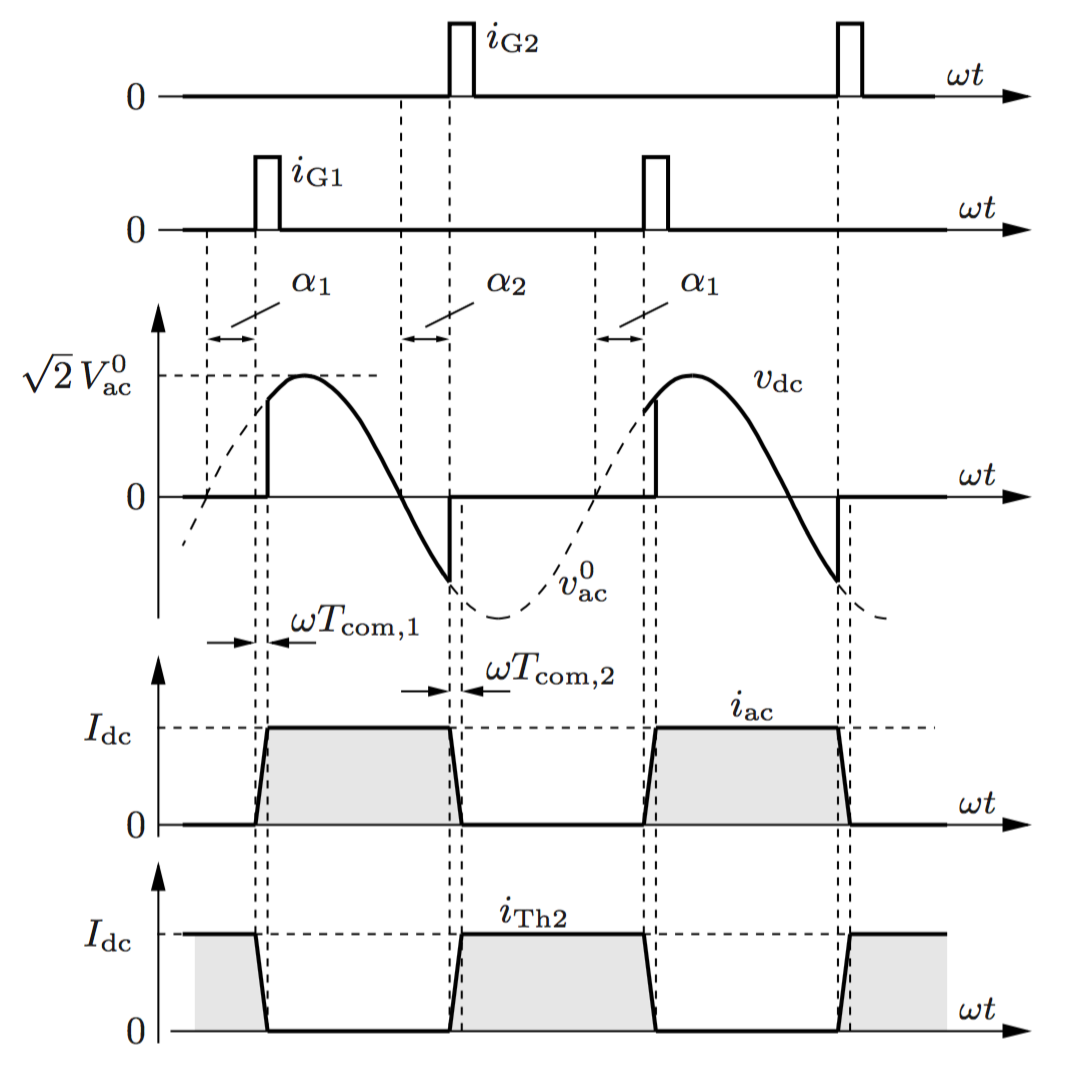
\includegraphics[scale=0.3]{ch3/4}
				\captionof{figure}{} 
				\end{wrapfigure}
				When $L_{ac} \neq 0$, commutation takes a certain time. During these intervals, both thyristors conduct simultaneously. The beginning of the rise of current $i_{ac}$, which is controlled by $\alpha _1$; and the beginning of the drop of current controlled by $\alpha _2$ follow the equation of the left mesh:
				\begin{equation}
					v_{ac}^0 = \sqrt{2} V_{ac}^0 \sin \omega t = L_{ac} \frac{di_{ac}}{dt}. 
				\end{equation}
				The rise time can be obtained by means of an integral:
				\begin{equation}
				\begin{aligned}
					&\int _{\alpha _1} ^{\alpha _1 + \omega T_{com,1}} \sqrt{2} V_{ac}^0 \sin \omega t \, d\omega t = \int _0^{I_{dc}} \omega L_{ac} \, di_{ac}\\ \Rightarrow\quad &\omega T_{com,1} = \arccos \left( \cos \alpha _1 - \frac{\omega L_{ac}}{\sqrt{2}V_{ac}^0}I_{dc} \right) - \alpha _1
					\end{aligned}
				\end{equation}
				We can see that $v_{dc}$ is only affected by the rises. The average output voltage drop due to commutation is: 
				\begin{equation}
					\Delta V_{com} = \frac{1}{2\pi} \int _{\alpha _1} ^{\alpha _1 + \omega T_{com,1}} L_{ac} \frac{di_{ac}}{dt} \, d\omega t = \frac{\omega L_{ac}}{2\pi} I_{dc}. 
				\end{equation}
				If we take into account the voltage drop due to conduction in the thyristors, the expression of the average output voltage becomes:
				\begin{equation}
				V_{dc} = \underbrace{\frac{\sqrt{2}}{\pi} \frac{\cos \alpha _1 + \cos \alpha _2}{2} V_{ac}^0 - V_{Th,on}}_{V_{dc}^0(\alpha _1,\alpha _2)} - \underbrace{\left( R_{Th,on} + \frac{\omega L_{ac}}{2\pi} \right)}_{R_{i,dc}}I_{dc}
				\end{equation}
				This equation describes the Thevenin-equivalent DC voltage source of the AC voltage source, rectifier system.

				
	\section{Single-phase and three-phase thyristor bridges}
		\begin{wrapfigure}[11]{l}{9.7cm}
		\vspace{-5mm}
		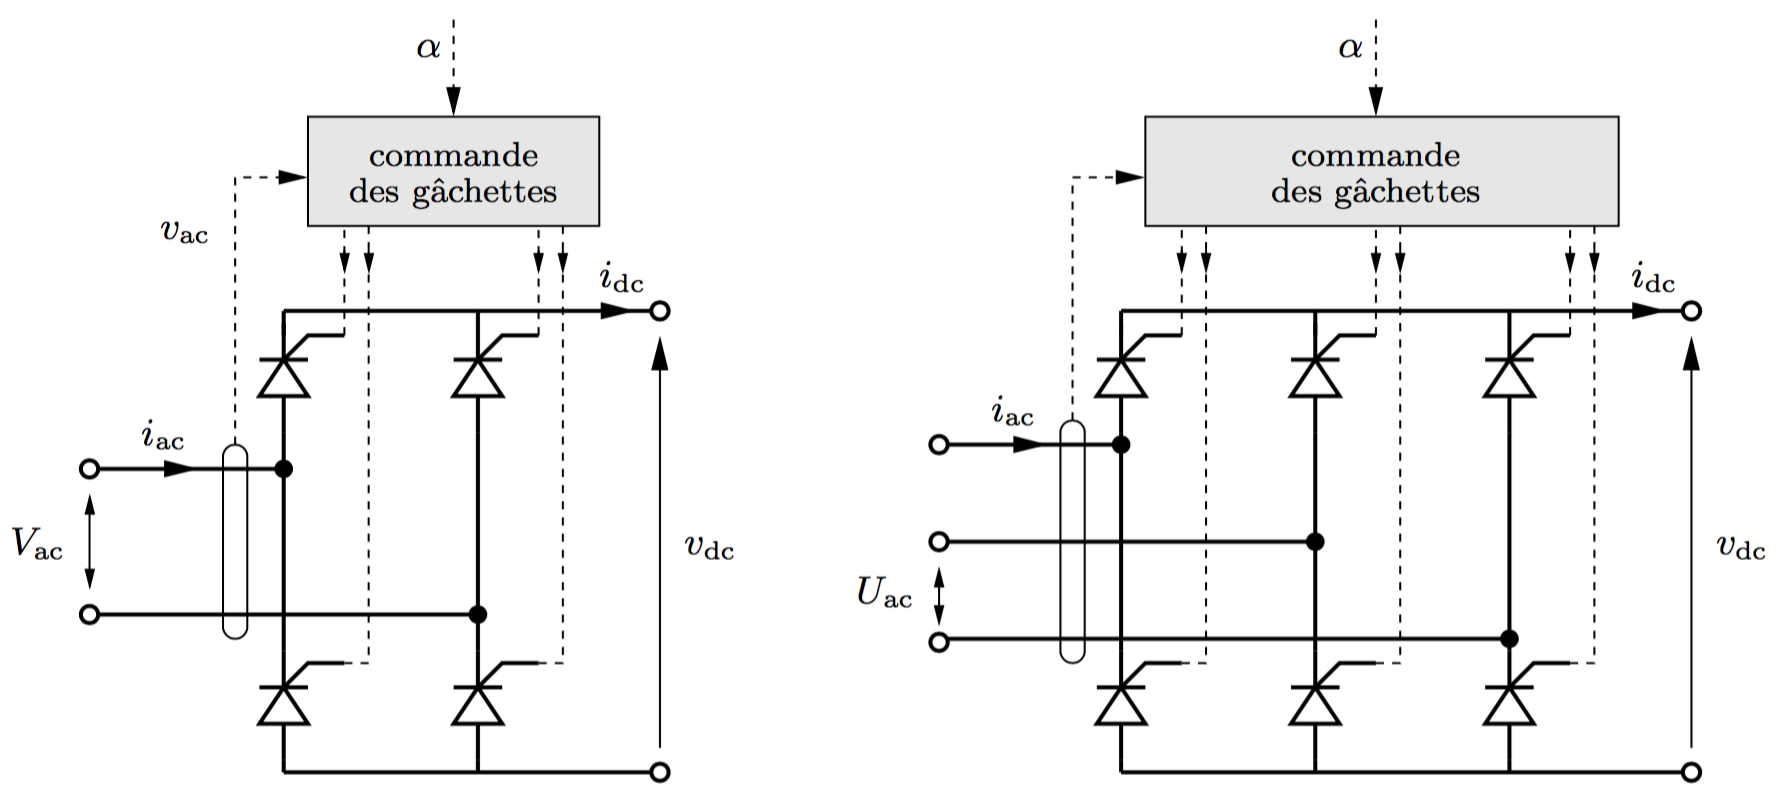
\includegraphics[scale=0.3]{ch3/5}
		\captionof{figure}{} 
		\end{wrapfigure}
		The layouts of these bridges are in the figure. The drive of the thyristors will control a parameter $\alpha$. This $\alpha$ is the lag of the beginning of conduction in the thyristor rectifier with respect to that of a diode rectifier with the same topology ($\alpha = 0$ for a diode). The distortion of the AC and DC quantities are composed of the same order of harmonics. We will consider a load inductive enough to avoid the discontinuity of the current.
		Depending on $\alpha$, we will have a rectifier or an inverter. A DC load able to furnish power will be required for the system to operate as an inverter. 
		
			\subsection{Rectifier operation}
				\subsubsection{Single-phase bridge and RLE load}
					We will assume an ideal AC voltage source. Under these conditions, a rectified current will only appear if $E_{dc} < V_{dc}$. \\
					
					\begin{itemize}
					\item[•] \textbf{Infinitely inductive load}\\
					In \autoref{fig:3.6} we can observe the shapes of the waves for $\alpha \approx 45^{\circ}$. We note that when $v_{ac}$ goes trough 0 to become positive, Th2 and Th3 keep conducting because of the inductance and the thyristors waiting for their initiation. Once booted, conduction begins instantaneously and the other pair of thyristors is inversely-biased. A perfectly smooth $I_{dc}$ implies that $i_{ac}$ is a square-wave current. Nevertheless, the fundamental component $i_{ac,1}(t)$ is shifted with respect to $v_{ac}(t)$  by an angle $\varphi _1 = \alpha$. This induces a reactive power consumption proportional to $\sin \alpha$. Furthermore, we have $I_{ac,1} = \frac{2\sqrt{2}}{\pi}I_{dc}$. We must point out that a discontinuity of $i_{dc}(t)$ when $v_{dc}(t)<0$ is avoided because we used a big inductance (even if $\alpha \neq 0$). 
					\end{itemize}
					
					\begin{center}
					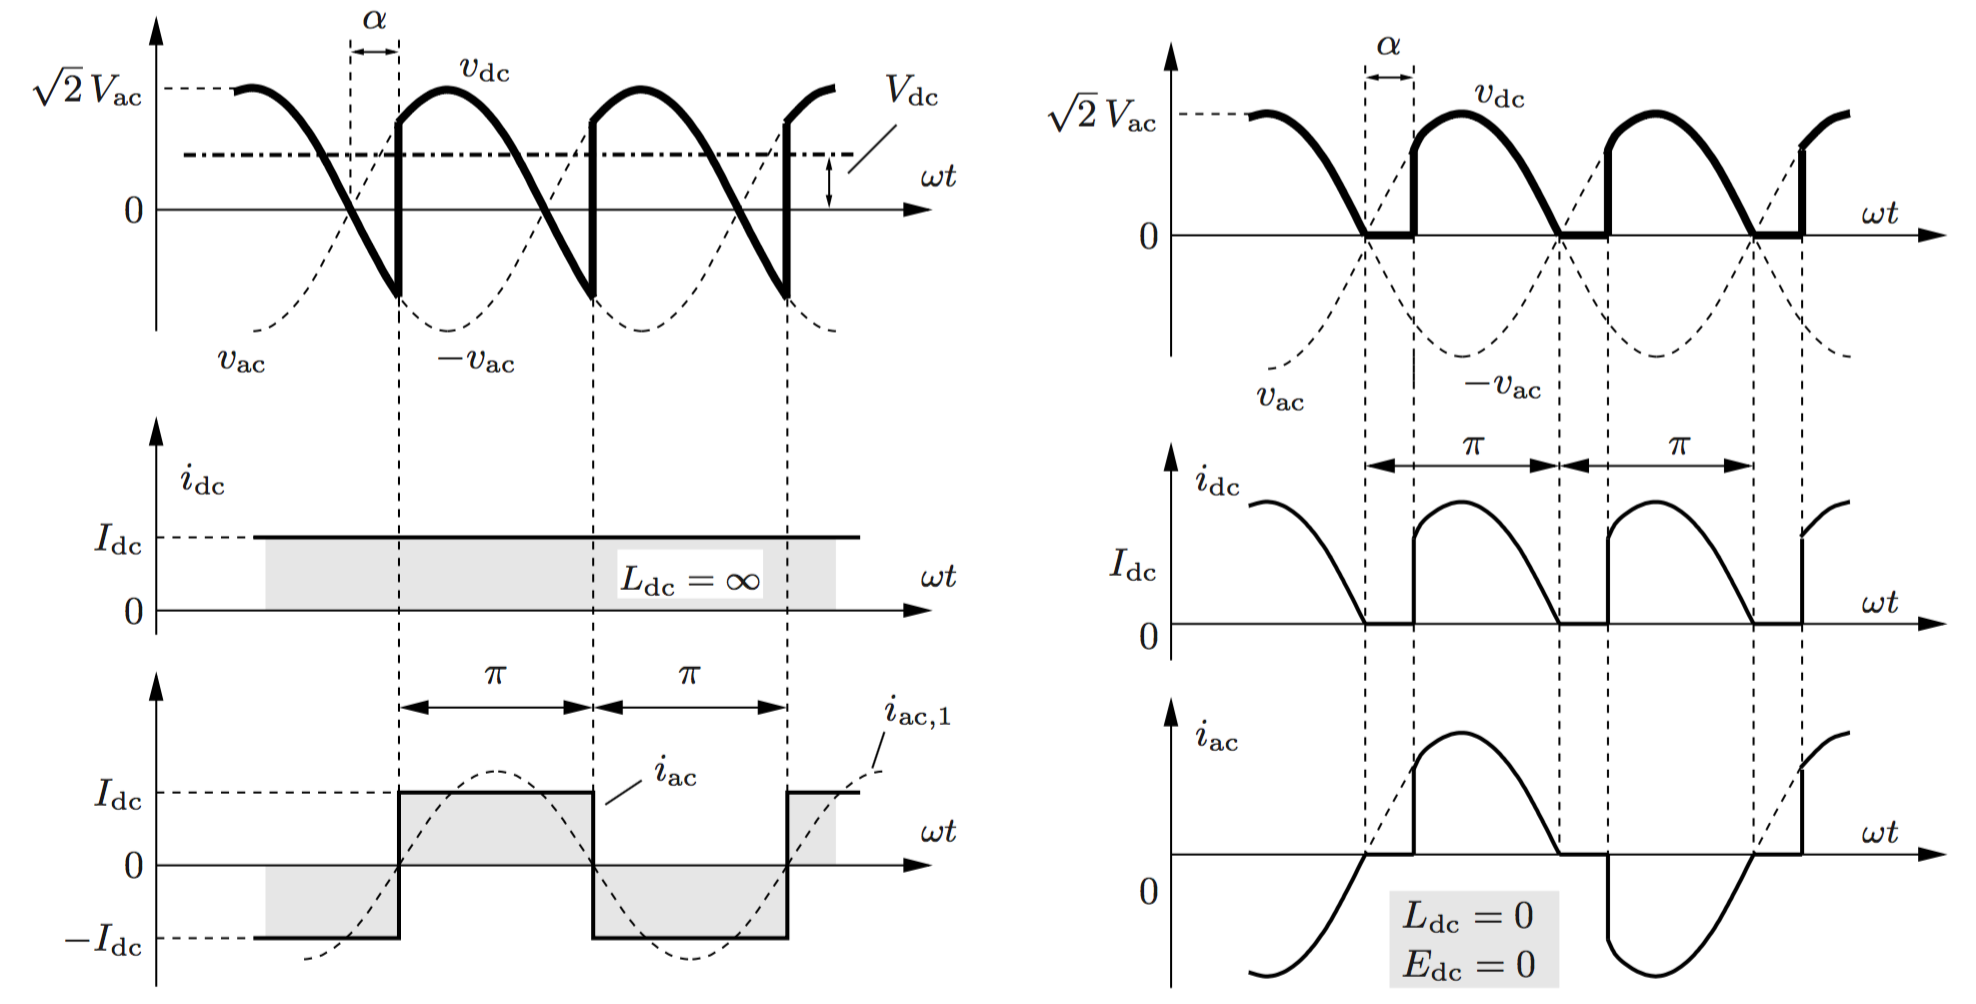
\includegraphics[scale=0.3]{ch3/6}
					\captionof{figure}{}
					\label{fig:3.6}
					\end{center}
					
					\begin{itemize}
					\item[•] \textbf{Purely resistive load}\\
					In this case, conduction becomes discontinuous regardless of the choice of $\alpha$. This happens because neither the current nor the output voltage can invert (see in \autoref{fig:3.6} to the right). 
					\end{itemize}
					
				\subsubsection{Three-phase bridge and infinitely inductive load}
					\begin{wrapfigure}[12]{l}{5.5cm}
					\vspace{-5mm}
					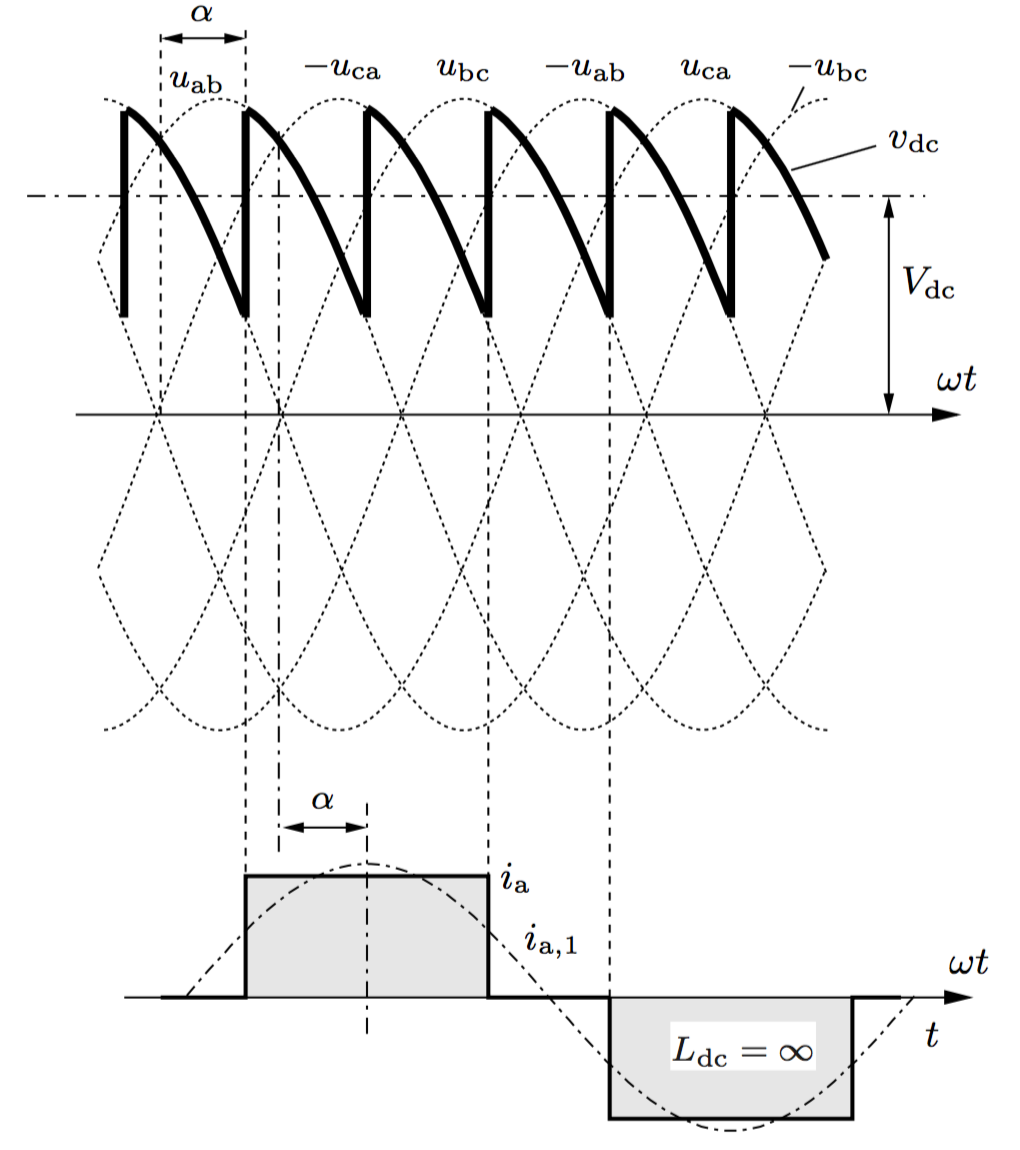
\includegraphics[scale=0.28]{ch3/7}
					\captionof{figure}{} 
					\end{wrapfigure}
					Here, we have the wave shapes when $\alpha \approx 40^\circ$. Under these conditions, the presence of a big inductance will induce a three-phase square wave current $i_{ac}(t)$ with a lag of $\phi _1 = \alpha$ with respect to the phase-to-neutral voltage of the first phase. We have $I_{ac,1} = \frac{\sqrt{6}}{\pi}I_{dc}$. it is easy to observe that the output voltage is never $<0$ as long as $\alpha < 60^\circ$ when we have an inductive load. If we had a purely resistive load, then current would be discontinuous. 
					
				\subsubsection{Average output voltage: basic equations (continuous conduction)}
    				If we have continuous conduction we only need to add $\alpha$ to the integration limits of the equivalent diode bridge:				
					\begin{equation}
					\begin{aligned}
					single-phase &: \frac{1}{\pi} \int _{-\pi /2+\alpha}^{\pi /2 +\alpha} \sqrt{2}V_{ac}\cos\omega t\, d\omega t = \frac{2\sqrt{2}	}{\pi} V_{ac}\cos \alpha \\
					three-phase &: \frac{3}{\pi} \int _{-\pi /6+\alpha}^{\pi /6 +\alpha} \sqrt{2}U_{ac}\cos\omega t\, d\omega t = \frac{3\sqrt{2}	}{\pi} U_{ac}\cos \alpha
					\end{aligned}
					\end{equation}
		
					\begin{wrapfigure}[7]{r}{4.7cm}
					\vspace{-5mm}
					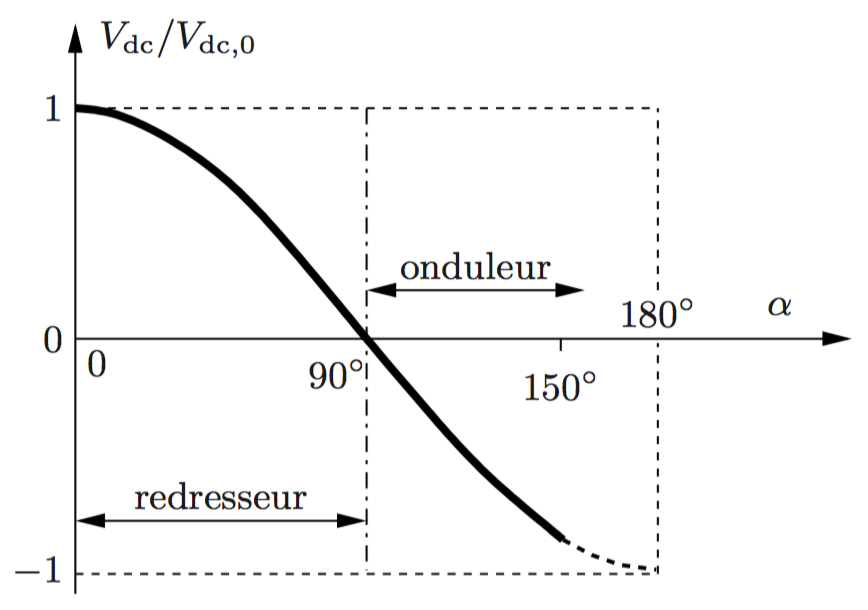
\includegraphics[scale=0.3]{ch3/8}
					\captionof{figure}{} 
					\end{wrapfigure}
					The maximum average corresponds to an $\alpha = 0$ and it will be zero when $\alpha = \pi /2$. If $\alpha > \pi /2$ the average becomes negative. the progression of the average output voltage with $\alpha$ appears in the figure.
					If our source has an inner inductance and if we take into account the conduction losses in the thyristors, the model of the system will become a bit more complex. To simplify it a bit we will use the Thevenin theorem
					
					\newpage
					
			\subsection{Inverter operation (non-autonomous)}
				\begin{wrapfigure}[13]{l}{5.5cm}
				\vspace{-5mm}
				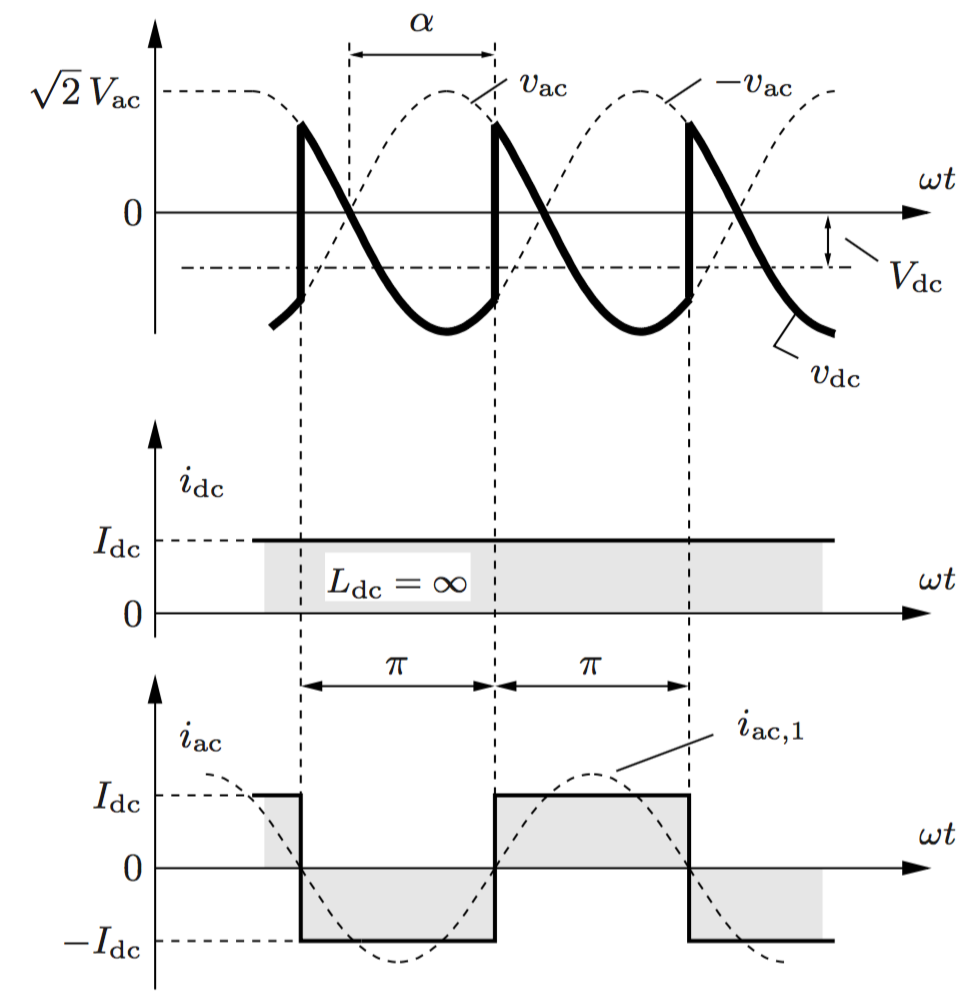
\includegraphics[scale=0.28]{ch3/9}
				\captionof{figure}{} 
				\end{wrapfigure}
				The system operates as an inverter when $\alpha$ is between $90^\circ$ and $180^\circ$. The average output voltage is negative and the average power goes from the DC mesh to the AC mesh. On the side we can see the waves shapes when $\alpha \approx 135^\circ$. Remember: the load must include an energy source such as the \textit{armature of a brushed DC machine}, here we consider a negative $E_{dc}$. As the rectified current is positive, the inequality $E_{dc}<V_{dc}$ is respected:
				\begin{equation}
					V_{dc} = E_{dc} + RI_{dc} \qquad \Rightarrow E_{dc} < V_{dc} < 0 
				\end{equation}
				The theoretical limit of $\alpha$ is $180^\circ$ but it is lower in practice because of the commutation intervals. We note that another AC voltage source is needed in order to control the thyristors. That is why they are called \textbf{semi-controllable} or \textbf{non-autonomous inverters}. Another consequence of the  employment of thyristors is that we are unable to furnish reactive power to the AC grid. 
				
					\subsubsection{Active and reactive power}
						If we consider a very inductive load (or DC source) and we neglect the commutation intervals and the losses in the bridge, the \textbf{active power} of the AC mesh will be:
						\begin{equation}
						\begin{aligned}
						single-phase &: V_{ac}I_{ac,1}\cos \alpha = V_{dc}I_{dc}\\
						three-phase &: \sqrt{3}U_{ac}I_{ac,1}\cos \alpha = V_{dc}I_{dc}.
						\end{aligned}
						\end{equation}

						The \textbf{reactive power} will be: 
						\begin{equation}
						\begin{aligned}
						single-phase &: Q_1 = V_{ac}I_{ac,1}\sin \alpha \geq 0\\
						three-phase &: Q_1 = \sqrt{3}U_{ac}I_{ac,1}\cos \alpha \geq 0.
						\end{aligned}
						\end{equation}
						The rectifier will always draw some reactive power and it will reach a maximum when $\alpha = 90^\circ$. this is the major disadvantage of these converters. The distortion of the output voltage will also be troublesome. For $\alpha = 90^\circ$, $v_{dc}$ will have a sawtooth shape with an average value equal to 0. 
						
	\section{Half controlled bridges (with diodes and thyristors)}
		\begin{wrapfigure}[10]{r}{9cm}
		\vspace{-5mm}
		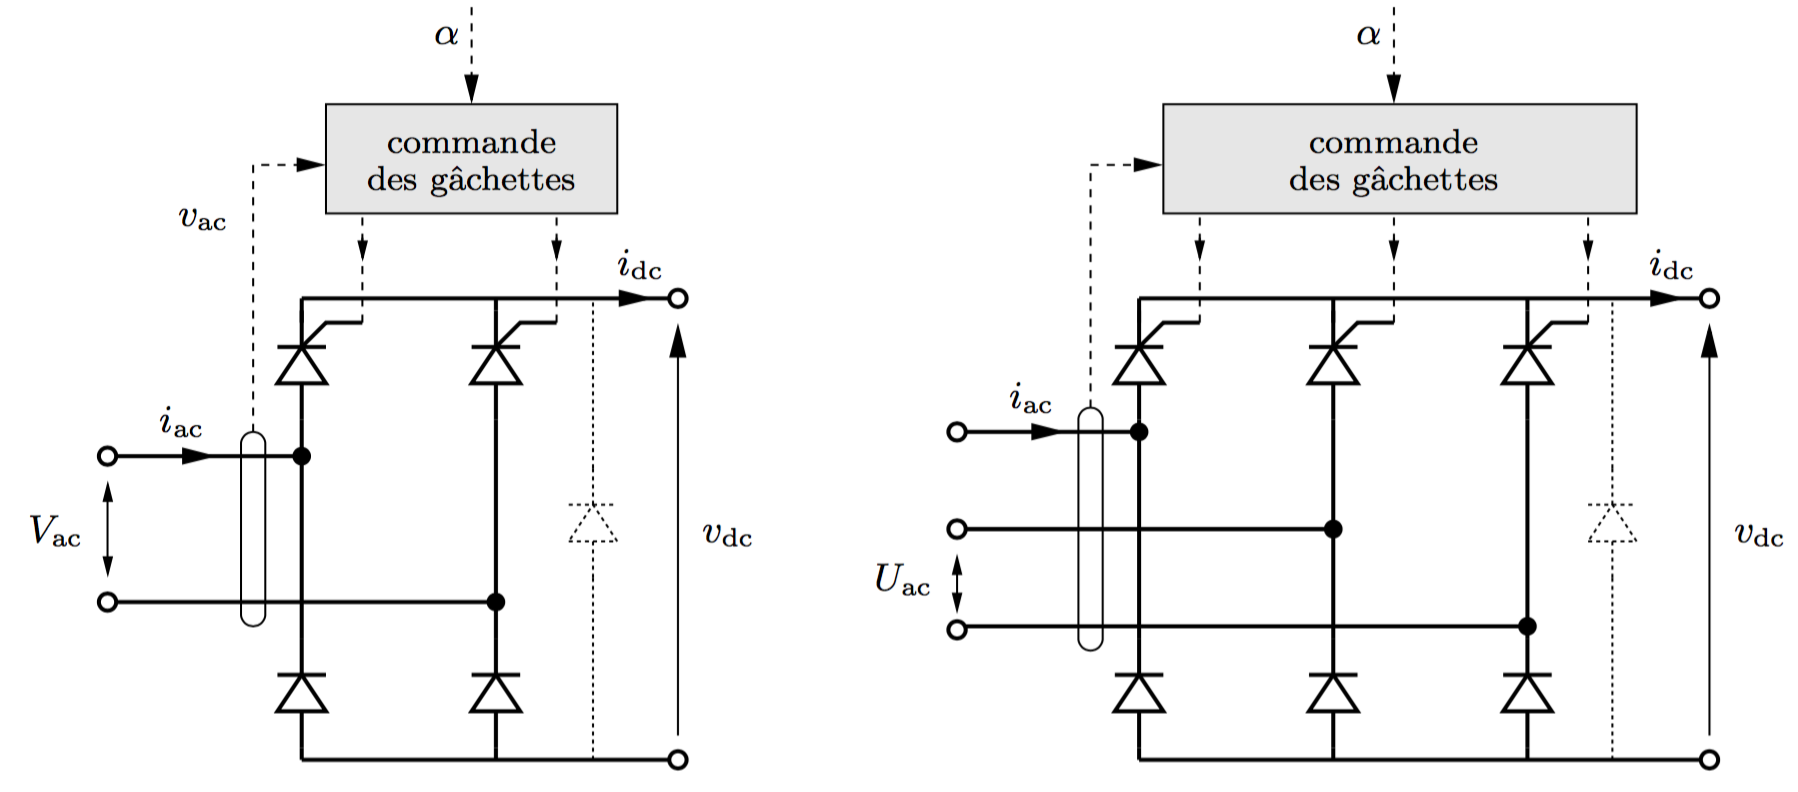
\includegraphics[scale=0.28]{ch3/10}
		\captionof{figure}{} 
		\end{wrapfigure}
		These bridges are composed of diodes and thyristors. We might also add a free-wheeling diode that will not have a big impact on the rectifier. Other than thyristors and diodes other components may be needed depending on the constraints. 
		
		\ \\ First, we will study the case of a single phase bridge with an infinitely inductive load, an ideal AC voltage source and ideal semi-conducting components. The wave shapes are represented in \autoref{fig:3.11}. In that figure we note that $v_{dc}(t)$ cannot be negative. If $\alpha \neq 0$, 
		
		\ \\
		
		\begin{wrapfigure}[12]{l}{5cm}
		\vspace{0mm}
		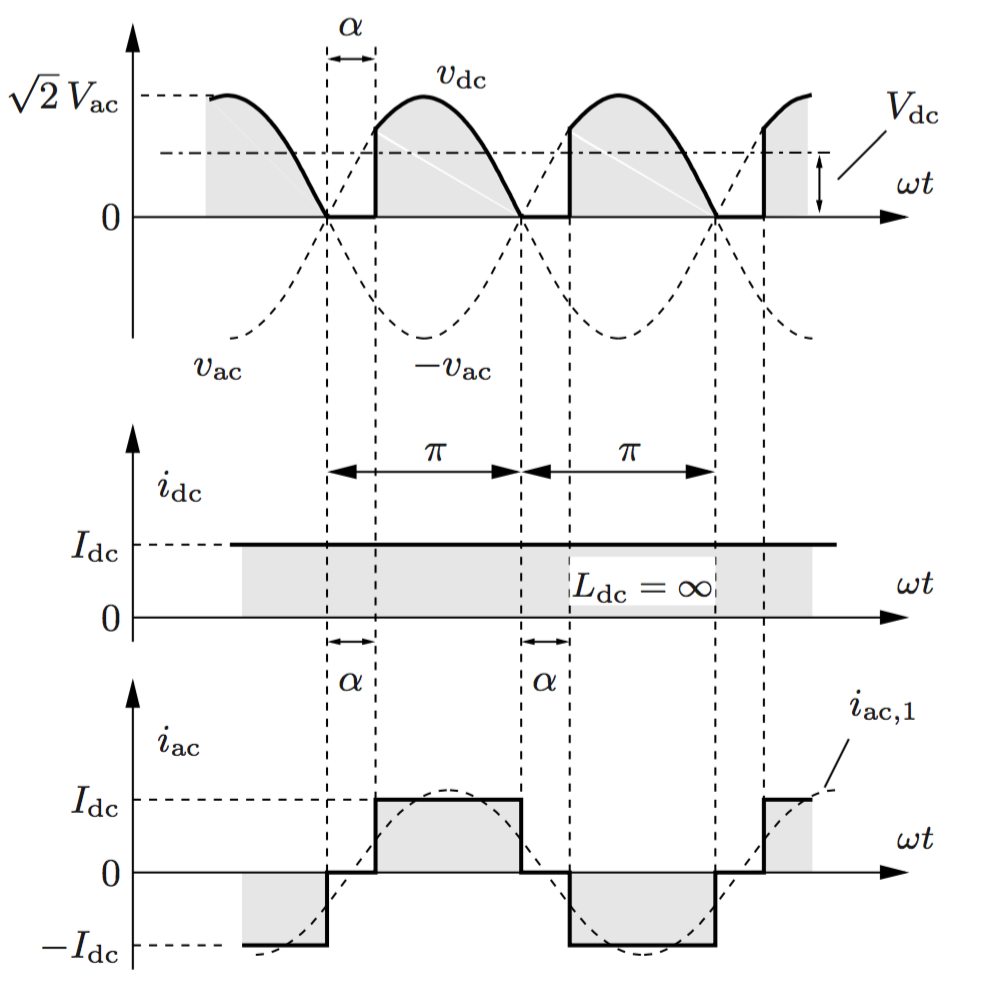
\includegraphics[scale=0.28]{ch3/11}
		\captionof{figure}{} 
		\label{fig:3.11}
		\end{wrapfigure}
		there are intervals without any output voltage. That happens when either the free-wheeling diode or a leg of the bridge short-circuits the system. The average output voltage is given by: 
		\begin{equation}
			V_{dc} = \frac{1}{\pi} \int _{-\pi /2 +\alpha} ^{\pi /2} \sqrt{2} V_{ac} \cos \omega t \, d\omega t = \frac{2\sqrt{2}}{\pi} V_{ac} \frac{1+\cos \alpha}{2}
		\end{equation}
		that means that the average output voltage of a thyristor bridge is the same as the average output voltage of a diode bridge.
		The rms value of the fundamental component of $i_{ac,1}$ is given by: 
		\begin{equation}
			I_{ac,1} = \frac{2\sqrt{2}}{\pi} \cos \frac{\alpha}{2} I_{dc}.
		\end{equation}
		Its lag angle $\phi _1 = \alpha /2$. In addition, the distortion of the AC current will increase $\alpha$. And the power balance will be: 
		\begin{equation}
			V_{ac}I_{ac,1}\cos\alpha /2= V_{dc}I_{dc}. 
		\end{equation}
		In this equation we find the $DPF = \cos \alpha /2$.
		
		As the instantaneous output voltage (and consequently its average) is always positive these bridges cannot work as inverters. Their advantage is a minor cost and complexity. \\
		
		In the case of a three-phase system the average output voltage is: 
		\begin{equation}
			V_{dc} = \frac{3}{\pi} \int _{-\pi /6 + \alpha}^{\pi /6} \sqrt{2} U_{ac} \cos \omega t \, d\omega t = \frac{3\sqrt{2}}{\pi}U_{ac} \frac{1+\cos \alpha}{2}
		\end{equation}
		which is also the average of the output of a diode and a thyristor rectifier.
		
	\section{Characteristics of triacs - AC choppers}
		\begin{wrapfigure}[10]{l}{7cm}
		\vspace{-5mm}
		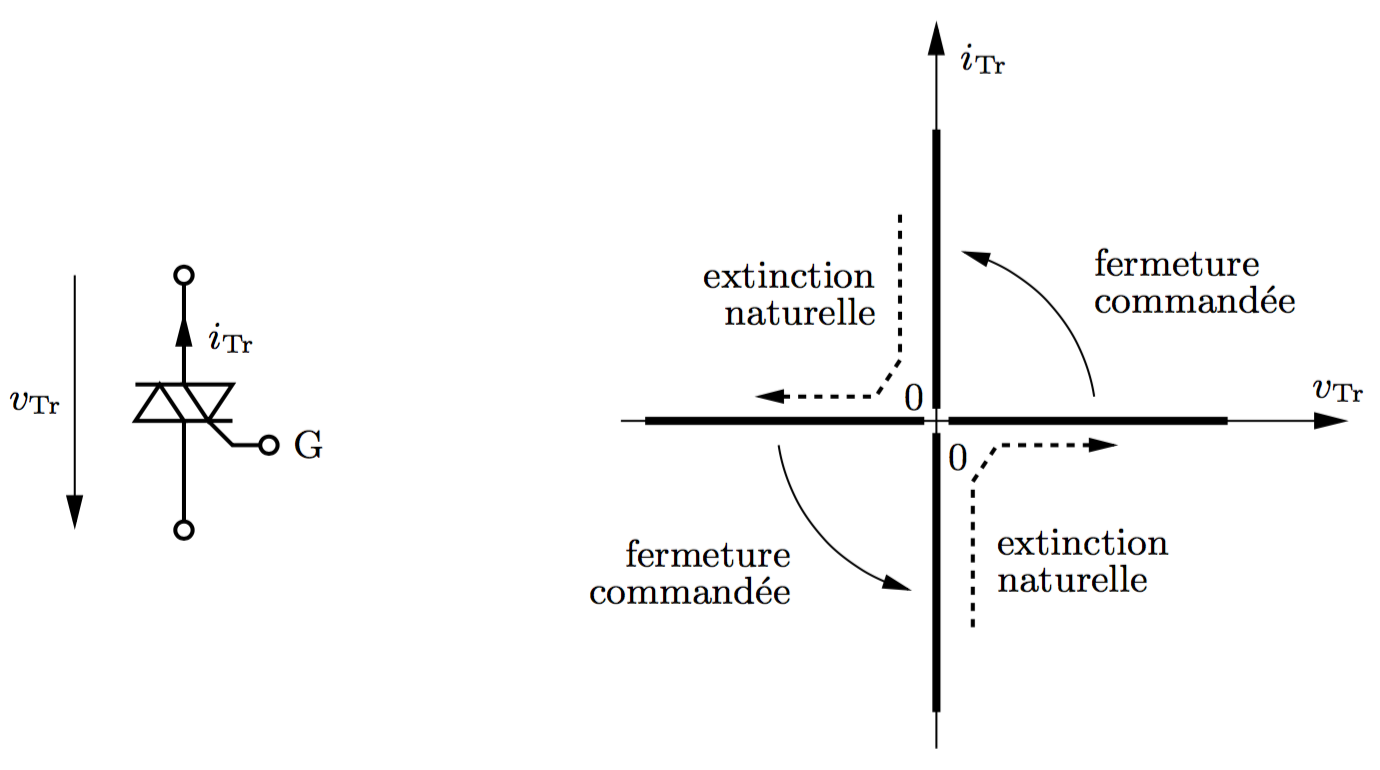
\includegraphics[scale=0.28]{ch3/12}
		\captionof{figure}{} 
		\label{fig:3.12}
		\end{wrapfigure}
		AC choppers carry out AC-AC conversions at a constant frequency whether in single-phase or three-phase. They are composed of triacs or, when the power consumption is too high for triacs, thyristor pairs (anti-parallel connection). This figure shows the bidirectionality of the triacs. In fact, they can conduct in one direction or the other depending on the sign of $v_{Tr}$ when the gate G gets a current impulsion. As triacs are composed of a diode and a thyristor it will turn itself off when the current becomes 0. 
		
			\subsubsection{Single phase AC choppers}
		 	\begin{wrapfigure}[7]{r}{9.8cm}
			\vspace{-5mm}
			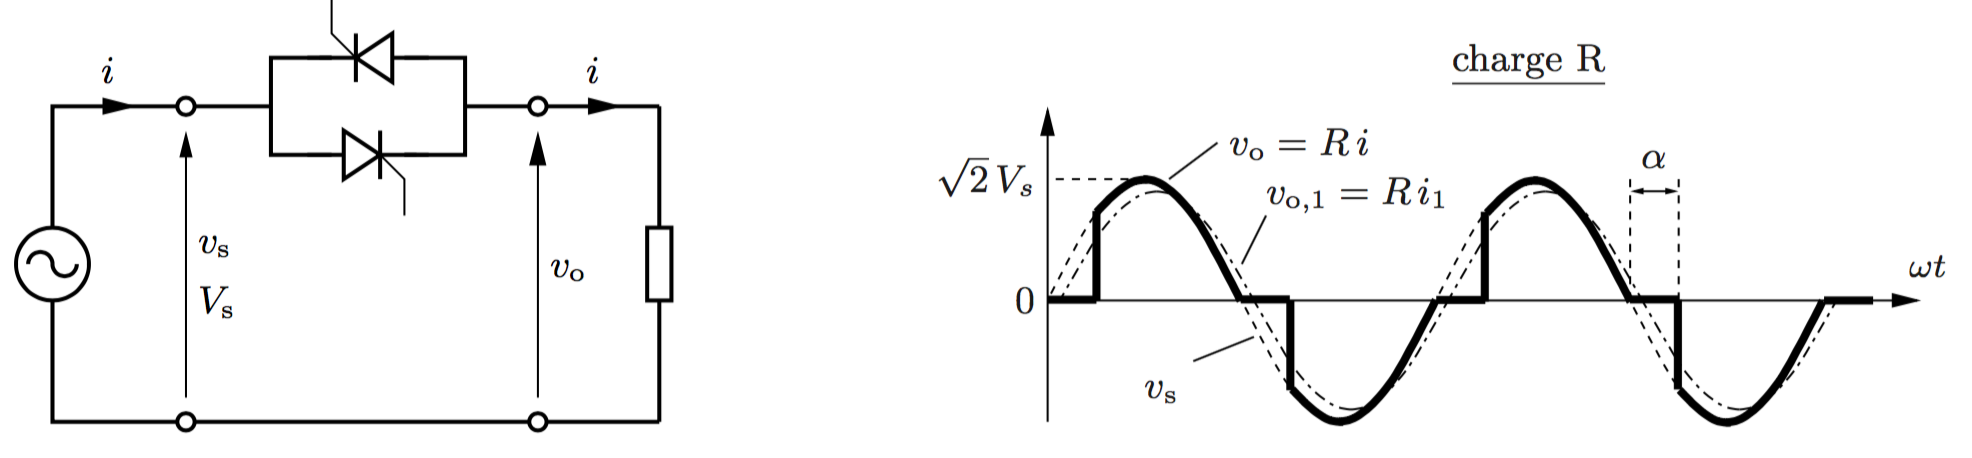
\includegraphics[scale=0.28]{ch3/13}
			\captionof{figure}{} 
			\label{fig:3.13}
			\end{wrapfigure}
			The circuit possesses 2 thyristors set in anti-parallel, which is the same as a triac. The output voltage $v_o(t)$ is controlled by the firing angle $\alpha$. That firing angle represents the time elapsed between the passage through 0 of the input voltage $v_s(t)$ and the sending of an impulsion to the thyristor ($f_o = f_s$). 
			
			\subsubsection{Purely resistive load}
				In \autoref{fig:3.13} we can observe the shapes of $v_o(t)$ and $v_{o,1}(t)$ when we have a purely resistive load $v_o(t) = Ri(t)$. The rms values of the fundamentals will diminish and the shift with respect to $v_s(t)$ will increase with $\alpha$. The chopper will consume reactive power when it feeds solely a load R. The rms value of the fundamental $V_o$ is calculated as follows:
				\begin{equation}
					V_o = \sqrt{\frac{1}{\pi}\int _\alpha ^\pi v_s^2 \, d\omega t} = V_s \sqrt{1- \frac{\alpha}{\pi} + \frac{\sin 2\alpha}{2\pi}}. 
				\end{equation}
				Even harmonics don't appear in the specter because of the half wave symmetry and the THD of $v_o$ will increase with $\alpha$. That is the main disadvantage of choppers. 
	
	\section{Cycloconverters}
		\begin{wrapfigure}[12]{r}{8.3cm}
		\vspace{-5mm}
		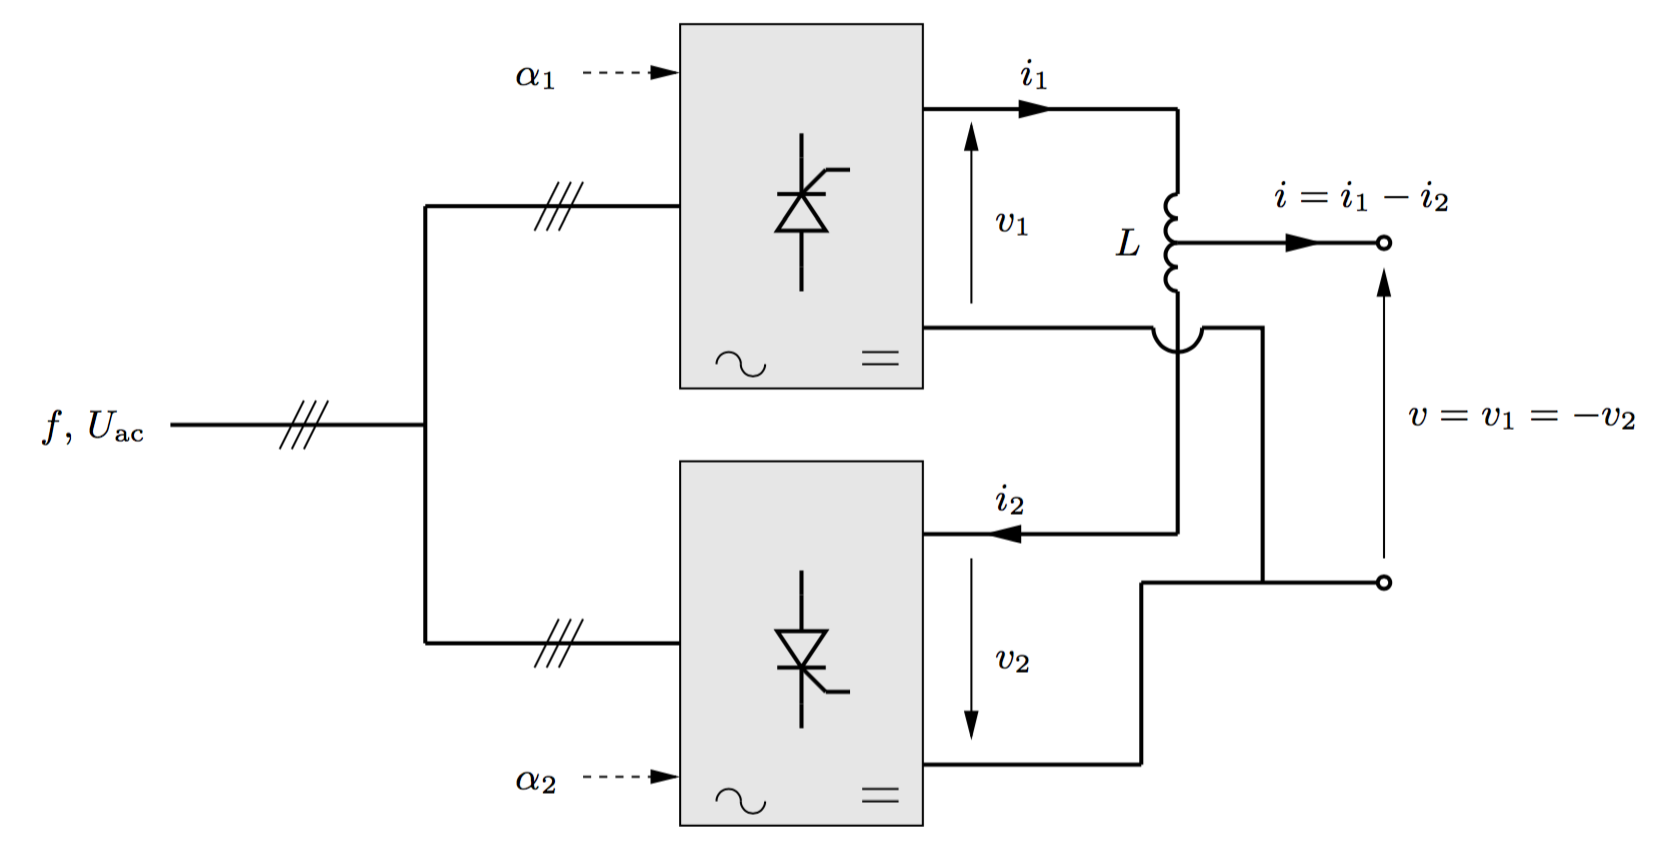
\includegraphics[scale=0.28]{ch3/14}
		\captionof{figure}{} 
		\label{fig:3.14}
		\end{wrapfigure}
		Cycloconverters are \textbf{direct frequency converters}, that is to say it doesn't need a DC bus. They are most often composed of thyristor bridges but it is not the only topology available. Let's consider three-phase to single-phase cycloconverters as the one in the figure. That cycloconverter has two thyristor bridges set head-to-tail. If we change  the firing angle $\alpha_1$ linearly and the firing angle $\alpha_2$ also changes linearly in order to complement $\alpha_1$, that is to say if $\cos \alpha _1 = - \cos \alpha 2$ and $\frac{d|\alpha _1|}{dt} = \frac{d|\alpha _2|}{dt} = \omega _1$, we obtain the average output voltage: 
		\begin{equation}
			v(t) = 1.35 U_{ac} \cos \alpha _1 (t) = 1.35 U_{ac} \cos (\omega _1 t + \gamma). 
		\end{equation}
		As $v_1(t) \neq v_2(t)$, a parasite current appears. The effect of this parasite can be limited through various means such as adding an inductance. We will create our sinusoidal voltage by assembling pieces of the six phase to phase voltages. If the signal isn't too distorted, the fundamental output frequency $f_1$ must be limited to one third or to 40\% of the source frequency. That is shown in this figure. 
		
		\begin{center}
			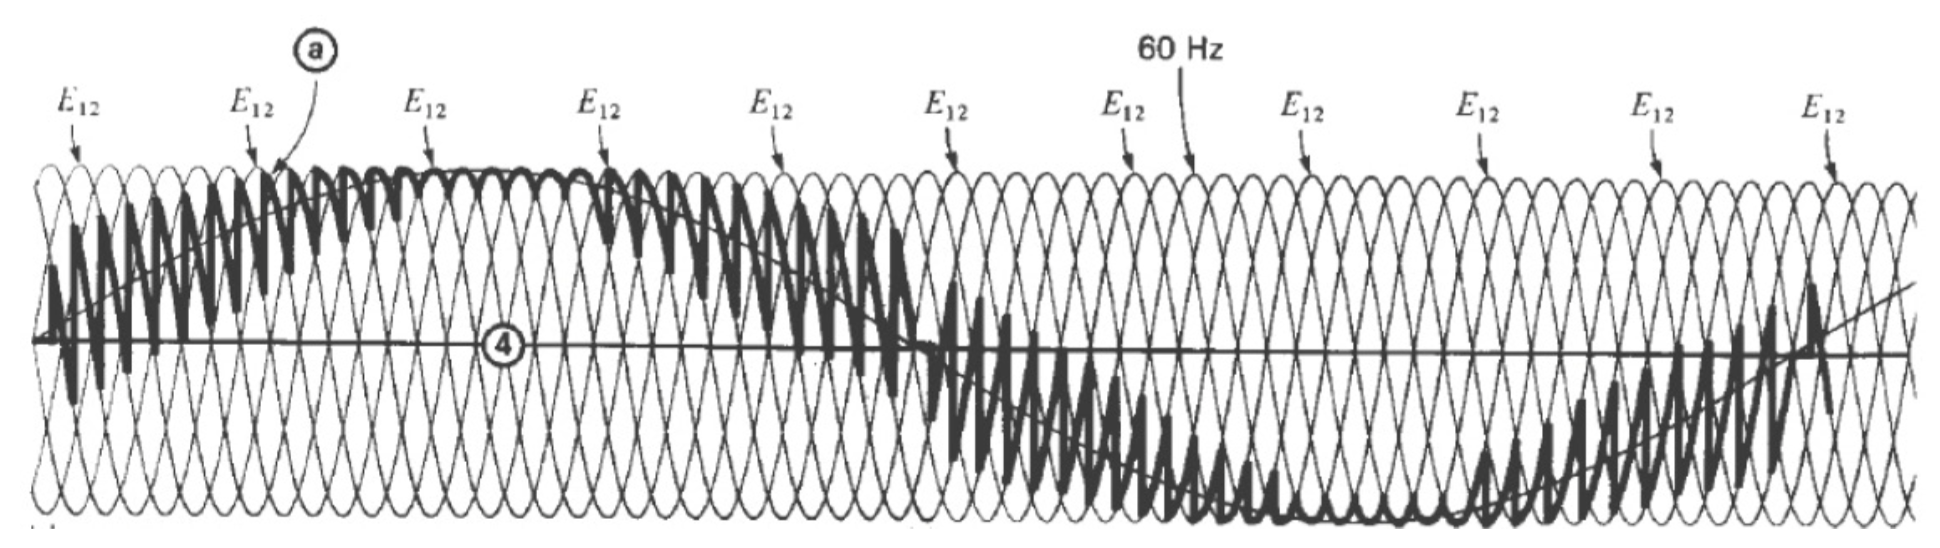
\includegraphics[scale=0.3]{ch3/15}
			\captionof{figure}{}
		\end{center}

%%%%%%%
% Ch4 %
%%%%%%%

\chapter{Universal bridges}
	\begin{wrapfigure}[5]{l}{6 cm}
	\vspace{-5mm}
	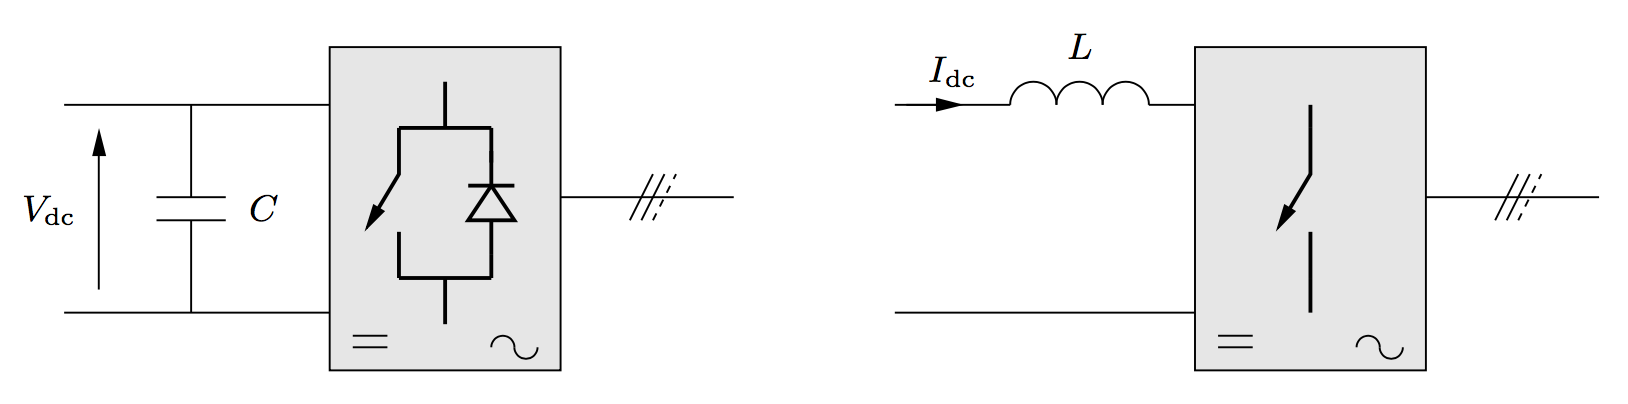
\includegraphics[scale=0.2]{ch4/1}
	\captionof{figure}{}
	\end{wrapfigure}
	The \textbf{autonomous inverters} most of times have bridges composed of fully controllable switches. They can be fed by a DC voltage source (voltage-source converter, VSC) or by a DC current source (current-source converter, CSC). Both models differ on the presence of a capacitor or an inductor in the entry bus. They can work as \textbf{rectifiers}. \textbf{Multi-quadrant} choppers, which are employed to control DC motors, have the same topology and a similar control. 
	
	\begin{minipage}{0.5\textwidth}
		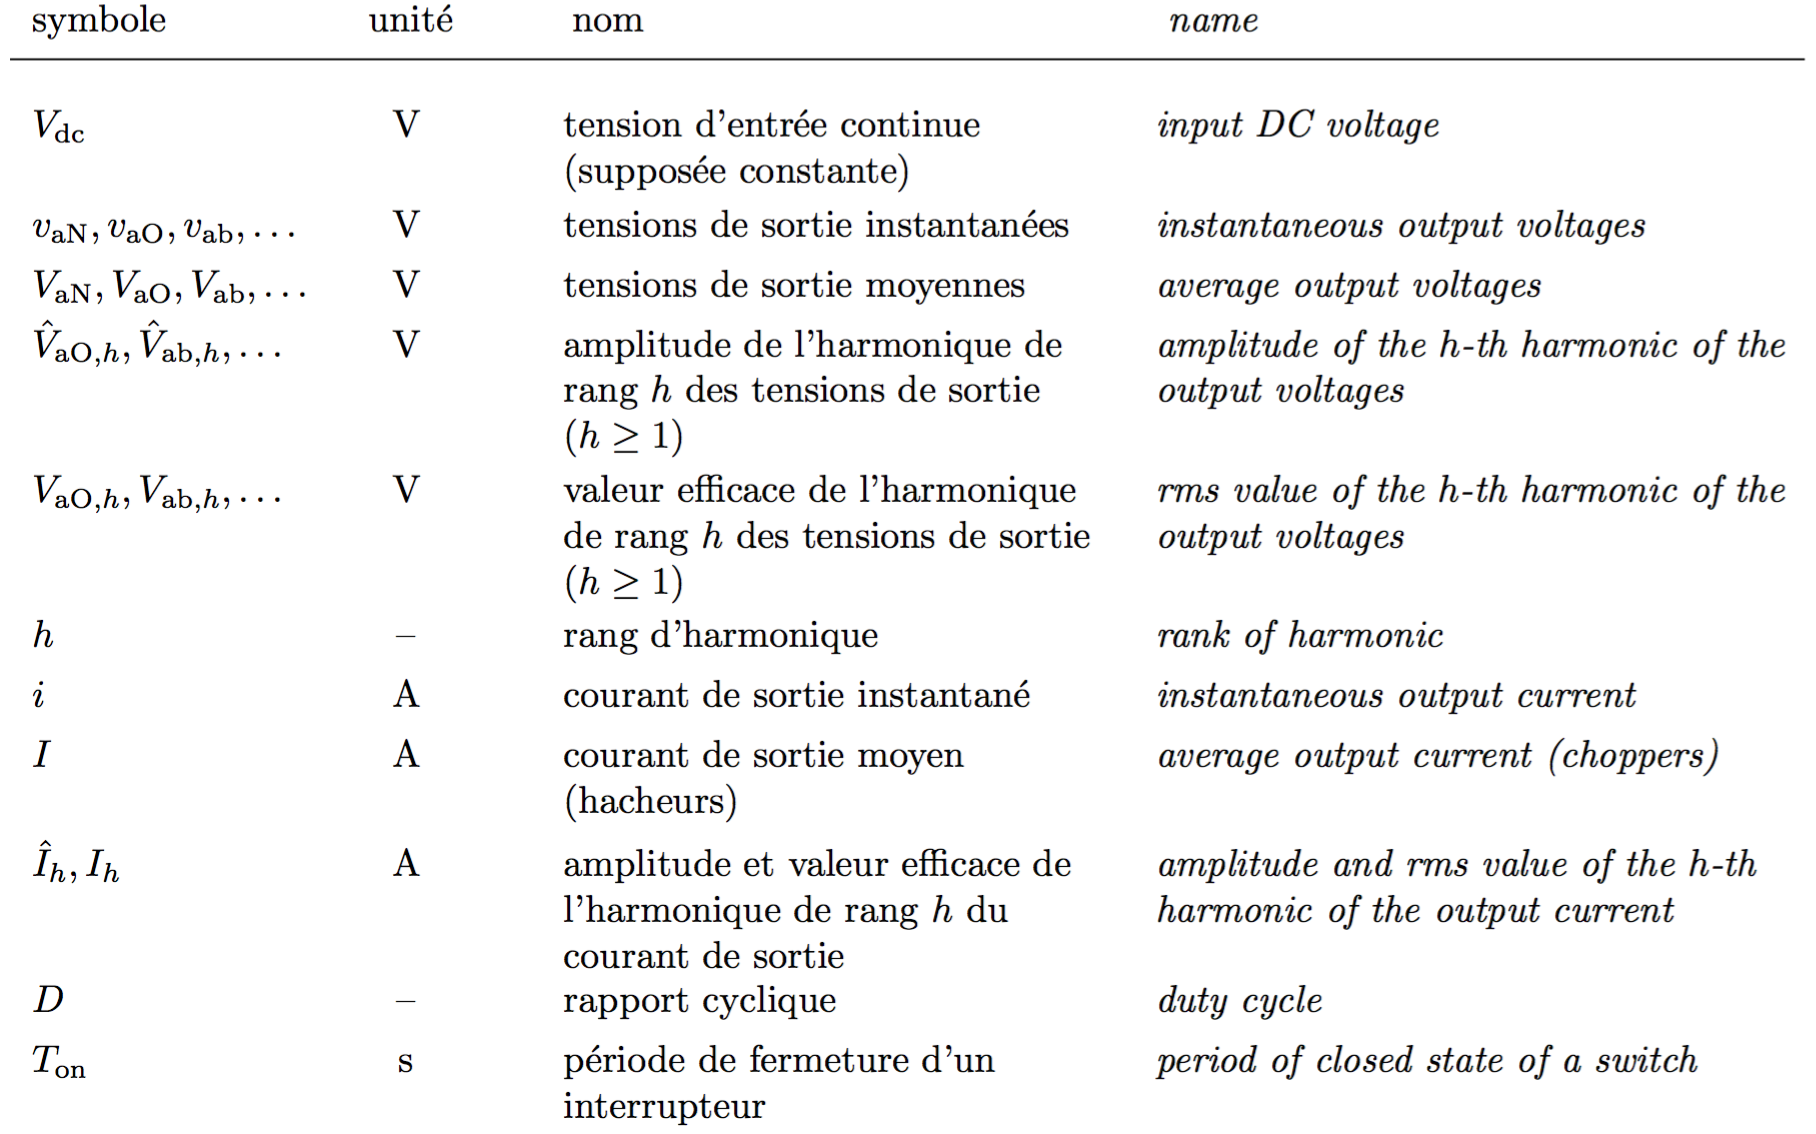
\includegraphics[scale=0.25]{ch4/2}
	\end{minipage}
	\begin{minipage}{0.5\textwidth}
		\vspace{3mm}
		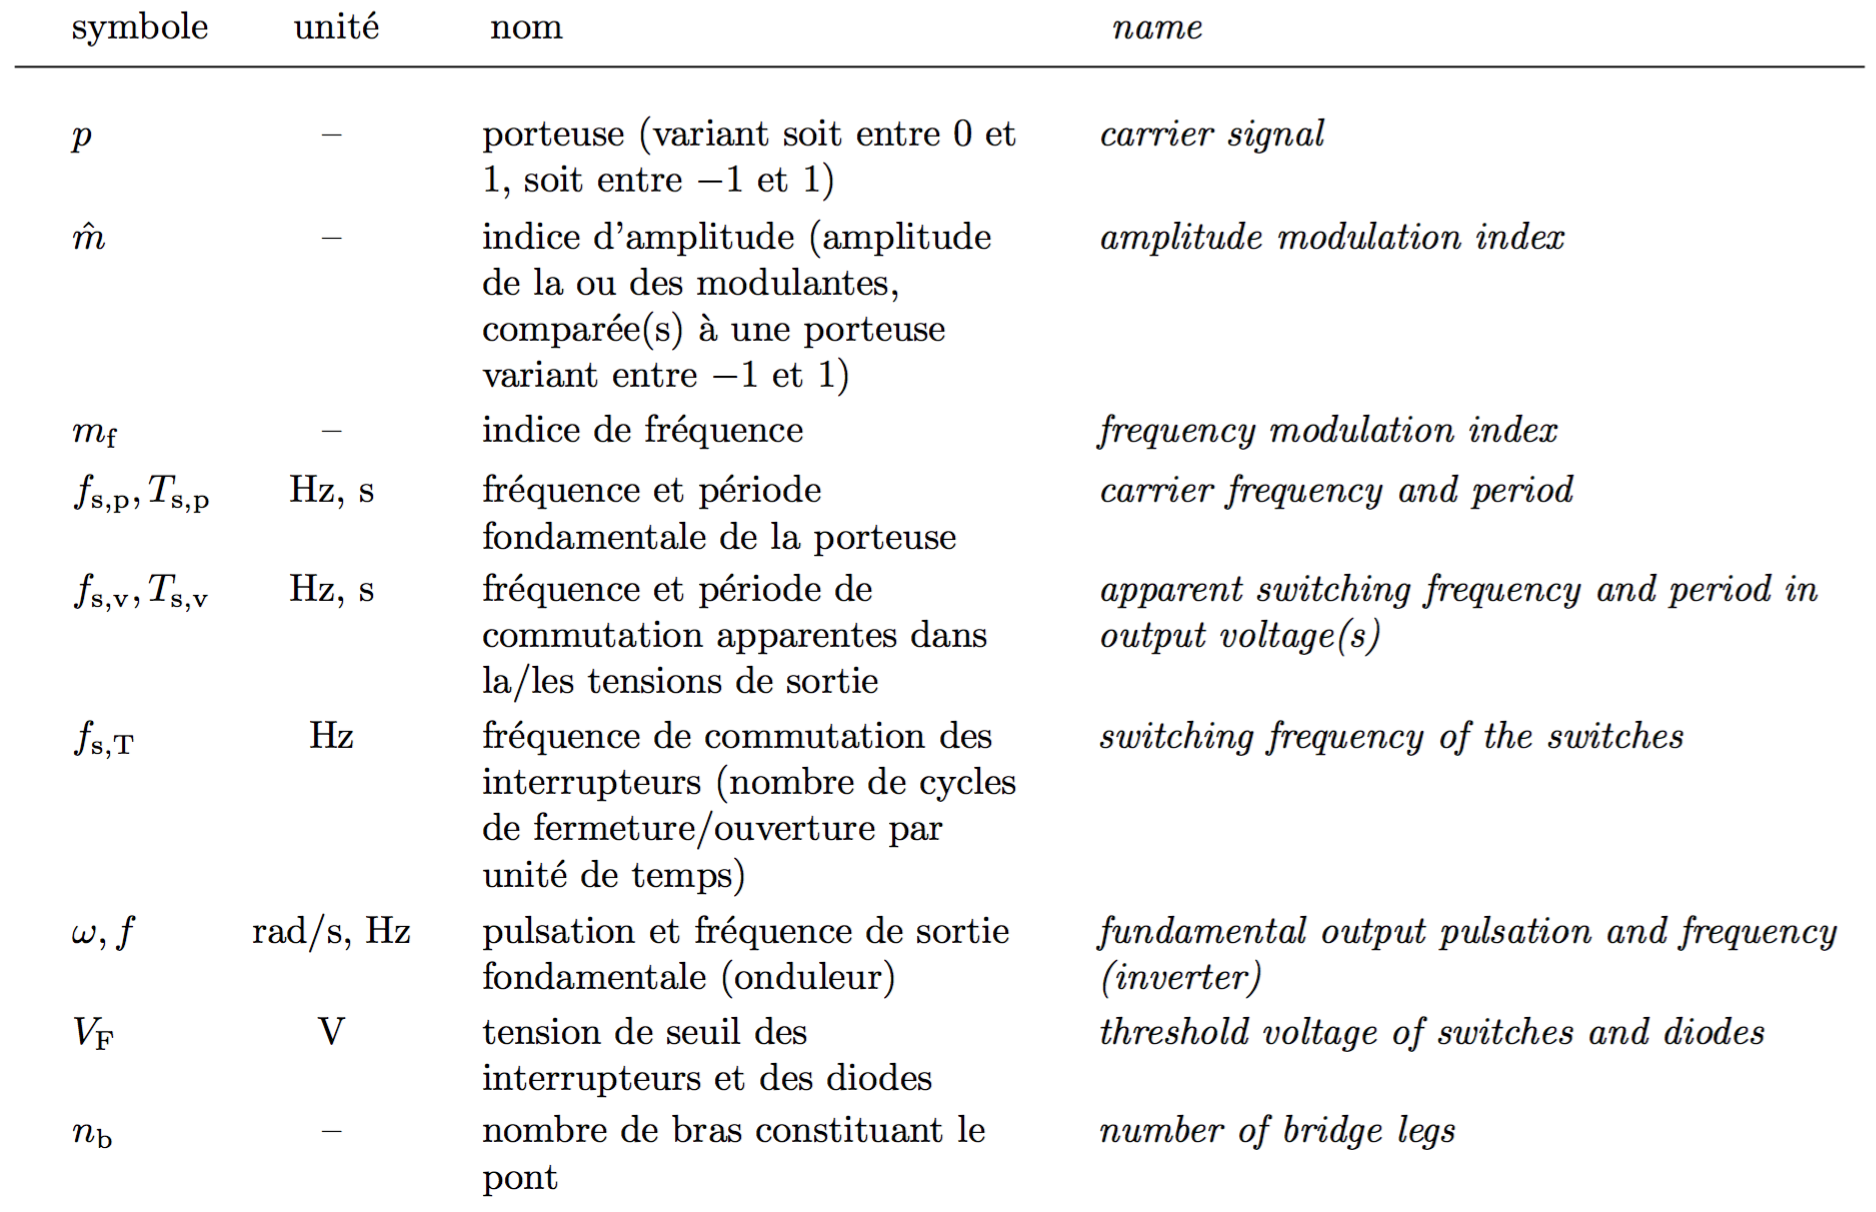
\includegraphics[scale=0.25]{ch4/3}	
	\end{minipage}
	\captionof{table}{List of symbols.}
	
\section{Characteristics of fully controllable switches}
	\begin{wrapfigure}[4]{r}{5 cm}
	\vspace{-5mm}
	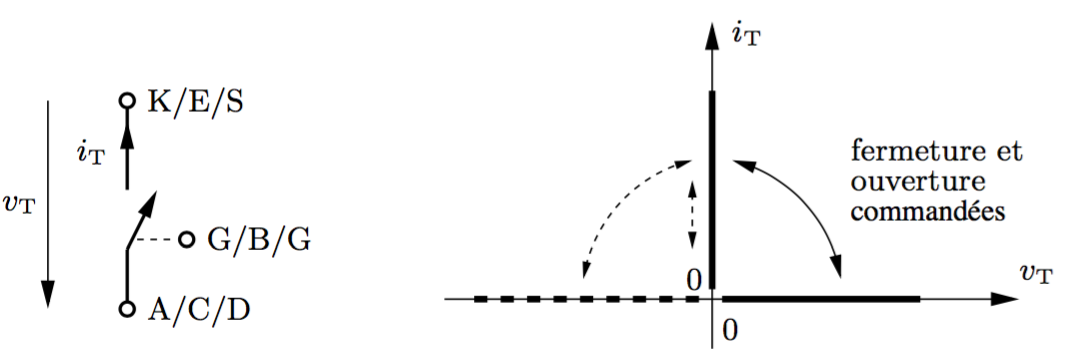
\includegraphics[scale=0.25]{ch4/4}
	\captionof{figure}{}
	\end{wrapfigure}
	Here is the ideal voltage versus current characteristic of a fully-controllable switch. The $2^{nd}$ quadrant doesn't matter to us because the voltage $v_T$ is negative and such an option is left out because there is a diode set in anti-parallel in the switch. \\
	
	\begin{wrapfigure}[6]{l}{6 cm}
	\vspace{-5mm}
	\includegraphics[scale=0.2]{ch4/5}
	\captionof{figure}{}
	\end{wrapfigure}
	All of them are \textbf{unidirectional} and the current cannot flow from the anode A to the cathode K, from the collector C to the emitter E or from the drain D to the source S. The \textbf{control electrode} (trigger G, base B or grid G) allows us to open or close the switch by means of a voltage or current. 
	
	The maximum voltage $V_{T,max}$ and current $I_{T,max}$ the switch can withstand are limited. In order to increase the rated power we can set multiple bridges in parallel or in series but then both the current and the voltage must be evenly distributed. Commutation between conducting and blocking takes a given interval of time that will limit the commutation frequency $f_{s,T}$. During those intervals, current and voltage will be the origin of \textbf{commutation losses}.
	
\section{Voltage-source converters: generalities}
	\subsection{Topologies and practical realisation}	
		\begin{wrapfigure}[12]{l}{7cm}
		\vspace{-5mm}
		\includegraphics[scale=0.2]{ch4/7}
		\captionof{figure}{}
		\end{wrapfigure}
		This figure represents 4 different bridges with 1,2 or 3 legs. Each leg has a bidirectional fully controllable switch set between the N and P input terminals. The point a, b and c are the output terminals. In the half bridge N and O are also output terminals.
		In order to avoid a short circuit two switches of the same leg cannot be closed at the same time. Otherwise a huge short-circuit current would flow through them and it may destroy them. Depending on which switches are closed and which are open different voltages will appear at the output.\\
		
		For the half bridge without midpoint we have $v_{aN} = 0$ or $v_{aN} = V_{dc}$. In the half bridge with midpoint, $v_{aN} = \pm V_{dc}/2$. In the H-bridge and the three-phase bridge, $v_{aN} = 0$ or $v_{aN} = \pm V_{dc}$. We can therefore create either DC or AC voltages with a chosen average value.  
		
		\begin{wrapfigure}[9]{r}{4cm}
		\vspace{-5mm}
		\includegraphics[scale=0.3]{ch4/8}
		\captionof{figure}{}
		\end{wrapfigure}
		\ \\ Here we can observe that each leg is composed of two unidirectional fully controllable switches (GTO, BJT, IGBT, MOSFET, ...), T1 and T2 as well as 2 free-wheeling diodes, D1 and D2 set in anti-parallel with the switches. In order to avoid a short-circuit caused by the diodes, voltage at the input must be \textbf{positive}. If T1 is closed then T2 must be open, a is therefore linked to the P bus and D2 is inversely-biased. If $i>0$, current will not go through T1 but through D1. The same thing happens if T2 is closed, T1 is open and a is linked to the N bus, D1 is inversely biased. If $i>0$ then it won't go through D2 but through T2. \\
		
		Let's focus on $v_{aO}(t)$ of the half bridge while considering $V_{dc}<0$ and constant. Under these conditions, if T1 is closed ($v_{aO(t)} = + V_{dc}/2$) and T2 is closed too ($v_{aO}(t) = -V_{dc}/2$) then for any value of the current $v_{aO}(t)$ depends only on the state of the switches. With an adequate switching frequency T we can get an average output between $+V_{dc}/2$ and $-V_{dc}/2$. \\
		
		As the commutation speed of a switch might be different from the other, there must be an interval of time during which both switches are open at the same times. Otherwise there would be short circuits very often (once every commutation period). We call that time \textbf{dead time} $t_{\Delta}$. During $t_{\Delta}$, the sign of the current will determine $v_{aO}$. 
		
	\subsection{Conduction in the semi-conducting components and associated losses}
		\begin{wrapfigure}[9]{l}{5.5cm}
		\vspace{0mm}
		\includegraphics[scale=0.3]{ch4/9}
		\captionof{figure}{}
		\end{wrapfigure}
		When the switches conduct, there is a slight \textbf{residual voltage} at its terminals (1 to 3V). That residual voltage induces a current flow and thus conduction losses. If the switch is open then the leakage current can be neglected.
		In this H-bridge, depending on the state (open or closed) of each switch and the current direction there are up to two times 9 possible combinations (4 $\times$ complementary states, 4 $\times$ a single leg closed). For example, if conduction takes place through D2 and D3 we have:
		\begin{equation}
			V_{ab} = -V_{dc}-V_{F,D2}-V_{F,D3}-(R_{on,D2}+R_{on,D3})i,
		\end{equation}
		where the instantaneous conduction losses (measured in W) are obtained by multiplying the Joule losses term by $i$. When current is negative, it will flow through T2 and T3, and thus:
		\begin{equation}
			V_{ab} = -V_{dc}+V_{F,T2}+V_{F,T3}-(R_{on,T2}+R_{on,T3})i. 
		\end{equation}
		
	\subsection{Commutation in a converter leg and associated losses}
		\begin{wrapfigure}[8]{r}{8cm}
		\vspace{-5mm}
		\includegraphics[scale=0.25]{ch4/10}
		\captionof{figure}{}
		\end{wrapfigure}
		Let's consider a half bridge whose midpoint is connected to an inductive load. With such a load current cannot change fast enough and during commutation it will flow through T1 or D2 or both: 
		\begin{equation}
			i = i_{T1}+ i_{D2}.
		\end{equation}		 
		The DC voltage:
		\begin{equation}
			V_{dc} = v_{T1} - v_{D2},
		\end{equation}
		where $v_{T1}$ are $v_{D2}$ near $0$ (in fact they are equal to the threshold voltage) during conduction and equal to $V_{dc}$ and $-V_{dc}$ during non-conduction intervals. During commutation intervals those voltages will go from one value to the other. The waves shapes show that, when T1 is closed, $i_{T1}$ starts increasing from 0 while D2 keeps conducting with $v_{D2} = 0$ and $v_{T1} = V_{dc}$. As long as D2 keeps conducting $-v_{D2}$ cannot rise to $V_{dc}$ and $v_{T1}$ cannot go down to 0. When it opens, $v_{T1}$ must rise 'til $V_{dc}$ in order for D2 to be directly-biased and conduct. \\
		
		During commutation, the instantaneous power consumption $p_{T1} = v_{T1}i_{T1}$ cannot be neglected and the total power consumption will be greater as $V_{dc}, i$ or the commutation intervals increase. As commutation losses are big and problematic the frequency at which those commutations take place will be of great relevance, that frequency is the \textbf{commutation frequency}. We can use the values on the datasheets to calculate the commutation losses in a leg. Those losses can be estimated with this equation:
		\begin{equation}
			P_{com} = f_{s,T} (E_{on,ref}+ E_{off,ref})\frac{V_{dc}}{V_{dc,ref}}\frac{i}{i_{ref}},
		\end{equation}
		where the $E$ are the energies relative to the reference values.
	
\section{Choppers - pulse width modulation (PWM)}
	 \textbf{Pulse width modulation (PWM)} is one of the methods available to control a converter leg. The commutation frequency remains constant and in each leg, the commutation period ($T_{s,T} = 1/f_{s,T}$) is split in 2 parts. During the first part the upper switch is closed and then the lower switch is closed. If we modulate the interval duration of the sub-intervals then we can generate an average voltage. \\
	 
	 The voltages are distorted by lots of harmonics because of commutation. With the aid of inductive loads the current can be rendered smoother. If we control the current through hysteresis, the commutation frequency is not constant and harmonics have a variable frequency. \\
	 In order to do an \textbf{intersective PWM} we have to determine the time when a switch commutes in each leg. We do that by comparing the \textbf{carrier p(t)} (a triangular signal of frequency $f_{s,p}$ and the \textbf{modulator} (the desired voltage). In the single-phase H-bridges we can use the same modulator for both legs (bipolar modulation) or 2 distinct modulators (unipolar modulation) with the same carrier. A \textbf{three-phase} inverter/rectifier has three modulators that constitute a balanced three-phase system. \\
	 
	 When we control the analogical electronics, the comparison between p(t) and m(t) is direct. With numerical electronics, we get the same result without the need of a comparison (duty cycle). 
	 
	 \subsection{Half bridge}
	 	\subsubsection{Without midpoint}
	 		\begin{wrapfigure}[8]{l}{6.5cm}
			\vspace{-5mm}
			\includegraphics[scale=0.2]{ch4/6}
			\captionof{figure}{}
			\end{wrapfigure}
			
			As the output voltage $v_{aN}(t)$ is always either positive or null, we use a triangular carrier p(t) that varies between 0 and 1. The modulator m(t) should change slowly (constant over a commutation period $T_{s,p}$) with respect to the carrier. When $m(t) > p(t)$, the upper switch of the leg is closed and $v_{aN} = V_{dc}$. When $m(t) < p(t)$, the closed switch is the closed one $v_{aN} = 0$. We consider that m(t) will also fluctuate between 0 and 1 in such a way that p and m intersect each other twice by commutation period $T_{s,p}$ and the switches will open and close themselves at the same frequency. We also find that frequency in $v_{aN}$ : 
			\begin{equation}
				f_{s,p} = f_{s,T} = f_{s,v}. 
			\end{equation}
			We will introduce a new parameter, the \textbf{duty cycle} of the switch. The duty cycle is the fraction of time during which the switch is closed ($0<D_x<1$). If we neglect the dead time of the switches: 
			\begin{equation}
				D_1 = \frac{T_{on,1}}{T_s} \qquad and \qquad D_2 = \frac{T_{on,2}}{T_s} = \frac{T_s - T_{on,1}}{T_s} = 1 - D_1.
			\end{equation}
			By convention, D (without any number) is the duty cycle of the upper switch, that is to say $D = D_1$. In this case:
			\begin{equation}
				D(t) = m(t). 
			\end{equation}
			We will do a \textbf{fast average} of $v_{aN}$ (average without commutation harmonics) as follows: 
			\begin{equation}
				V_{aN}(t) = \frac{1}{T_s}\int _{t-T_s/2}^{t+T_s/2} v_{aN}(t') \, dt'
			\end{equation}
			This average will change slowly with respect to $T_s$. It will be (approximately): 
			\begin{equation}
				V_{aN}(t) = m(t) V_{dc}. 
			\end{equation}
			
		\subsubsection{With midpoint}
			As $V_{aO}(t) = V_{aN}(t) - V_{dc}/2$ can be either positive or negative, this bridge can operate as an inverter/rectifier and as a chopper. If we take the same $p(t)$, we will always have $D(t) = m(t)$ and:
			\begin{equation}
				V_{aO}(t) = V_{aN}(t) - V_{dc}/2 = (m(t) - \frac{1}{2})V_{dc} \qquad and \qquad f_{s,p} = f_{s,T} =f_{s,v}
			\end{equation}
			
	\subsection{H-bridge}
		\subsubsection{Bipolar modulation}
		    In this case, we only need to use a single carrier $p(t)$ and a single modulator $m(t)$. If we control the switches diagonally ($T^a$ with $T_b$ and $T_a$ with $T^b$). This way, $v_{ab}(t)$ is either $V_{dc}$ or $-V_{dc}$. We have \textbf{bipolar commutation} because we combine 2 voltages. Diagonal commutation implies $v_{bO}(t) = - v_{aO}(t)$ and an output equal to twice that of half bridge with midpoint:
			\begin{equation}
				v_{ab}(t) = v_{aO}(t)-v_{bO}(t) = 2v_{aO}(t) \qquad \Rightarrow \qquad V_{ab}(t) = (2D(t)-1)V_{dc} = m(t) V_{dc},
			\end{equation}
			where D(t) is the duty cycle of the first leg. All the 3 $f_s$ are always equal.
			
		\subsubsection{Unipolar modulation}
			\begin{wrapfigure}[14]{l}{8cm}
			\vspace{-5mm}
			\includegraphics[scale=0.25]{ch4/11}
			\captionof{figure}{}
			\end{wrapfigure}
			We can also employ different modulators $m(t)$ for each leg. The carrier $p(t)$ will fluctuate between -1 and 1, with a modulator $m(t)$ for the control of the first leg and $-m(t)$ for the control of the second leg. When $m(t) > 0$, $v_{ab}(t)$ has positive impulsions of amplitude $V_{dc}$ ny commutation period. Therefore:
			\begin{equation}
				2 f_{s,p} = 2f_{s,T} = f_{s,v}.
			\end{equation}
			Let's note that there are intervals with a null output (the load is short-circuited). The output voltage is the same as before. \\
			
		\subsubsection{Bipolar versus unipolar modulation}
			\begin{wrapfigure}[8]{r}{7cm}
			\vspace{-5mm}
			\includegraphics[scale=0.2]{ch4/12}
			\captionof{figure}{}
			\end{wrapfigure}
			In the case of a bipolar modulation, there is a positive impulsion with length $DT_{s,T}$ and a negative impulsion $(1-D)T_{s,T}$ each commutation interval. If we have an unipolar modulation, then there are two impulsions with the same sign during each commutation period. The difference between both cases will be grow bigger as $|D-0.5|$ grows smaller.
			\newpage
			
	\subsection{Coverage in the voltage versus current plan}
		\begin{wrapfigure}[10]{l}{7.5cm}
		\vspace{-5mm}
		\includegraphics[scale=0.28]{ch4/13}
		\captionof{figure}{}
		\end{wrapfigure}
		\textbf{Choppers} carry out DC-DC conversions between a positive voltage $V_{dc}$ at the input and an average output that can be either positive or negative $V_{aN}, V_{aO}$ or $V_{ab}$. There is no constraint over the sign of $i(t)$ but there is a constraint on its average value: $-I_{T,min}\leq I \leq I_{T,max}$. Depending on its sign and that of the output voltage the power flow will go in one direction or the other. We can therefore distinguish 4 operation quadrants in the voltage versus current plan of choppers. 
		
	\subsection{Inductive load, distortion of the output current}
		\begin{wrapfigure}[8]{r}{9cm}
		\vspace{-5mm}
		\includegraphics[scale=0.25]{ch4/14}
		\captionof{figure}{}
		\end{wrapfigure}
		If the chopper has an RLE load fed by a voltage fluctuating between $V_{min}$ and $V_{max}$, with a period a period $T_{s,v}$ that depends on $f_{s,T}$ and the PWM employed. We consider a simplified system at steady-state and with a voltage $E=cst$. The instantaneous and average values are related by the following equations:\\
		\begin{equation}
			v(t) = Ri(t) + L\frac{di}{dt} + E \qquad and \qquad V = RI + E.
		\end{equation}
		If we subtract these equations we find the variations:
		\begin{equation}
			\Delta v(t) = R\delta i(t) + L\frac{d\Delta i}{dt}.
		\end{equation}
		$\Delta v(t)$ is constant during each interval and its value is $\Delta V_{max}$ during an interval $T_{v,max}$ and $\Delta V_{min}$ during $T_{v,min}$, with $T_{v,min} + T_{v,max} = T_{s,v}$. As the average $\Delta v(t) = 0$, we have:
		\begin{equation}
			\Delta V_{max}T_{v,max} + \Delta V_{min}T_{v,min} = 0 \qquad with \qquad \Delta V_{max} \geq 0 \ and \ \Delta V_{min} \leq 0
		\end{equation}
		$i(t)$ has sawtooth shape. Its rising slopes last $T_{v,max}$ and their descent lasts $T_{v,min}$. If the time constant $\tau = L/R \gg T_{s,v}$, the slope of the sides is almost constant and equals either $\Delta V_{max}/L$ or $\Delta V_{min}/L$. The peak-to-peak ripple $\Delta i(t)$ and $i(t)$ are:
		\begin{equation}
			\Delta I_{pp} = \frac{\Delta V_{max}T_{v,max}}{L} = -\frac{\Delta V_{min}T_{v,min}}{L}.
		\end{equation}
		
		The increase of $I_{rms}$ because of the ripple can be calculated as follows:
		\begin{equation}
		\begin{array}{c}
			I_{rms} = \sqrt{I^2+(\Delta I_{rms})^2} \qquad with \\
			\Delta I_{rms} = (\Delta i)_{rms} = \sqrt{\frac{1}{T_{s,v}}\int _{t_0}^{t0+T_{s,v}}(\Delta i)^2\, dt} = \Delta I_{pp} \sqrt{\int _{-1/2}^{1/2}x^2\, dx} 
		\end{array}
		\end{equation}
		Finally:
		\begin{equation}
			\Delta I_{rms} = \frac{1}{2\sqrt{3}}\Delta I_{pp}.
		\end{equation}
		Additional Joule losses in the loads' resistance R are $R(\Delta I_{rms})^2$. \\
		
		\textbf{Half bridge without midpoint} \qquad We have $T_{s,v} = T_{s,T}$, $V_{aN} = DV_{dc}, T_{v,max} = DT_s, \Delta V_{max} = V_{dc}-V_{aN}= (1-D)V_{dc}$ and thus:
		\begin{equation}
			\Delta I_{pp} = (1-D)D\frac{V_{dc}}{f_{s,T}L}= (1-D)\frac{V_{aN}}{f_{s,T}L}. 
		\end{equation}
		We can therefore decrease the ripple by increasing L and/or $f_{s,T}$. That ripple will also depend on D and it will reach a maximum for D = 0.5. \\
		
		\textbf{Half bridge with midpoint} \qquad We have $T_{s,v} =T_{s,T}, V_{aO} = (2D-1)V_{dc}/2, T_{v,max}=DT_{s,T}, \Delta V_{max} = V_{dc}/2-V_{aO = (1-D)V_{dc}}$ and thus:
		\begin{equation}
			\Delta I_{pp} = (1-D)D\frac{V_{dc}}{f_{s,T}L} = \frac{2(1-D)D}{2D-1}\frac{V_{aO}}{f_{s,T}L}.
		\end{equation}
		\ \\
		
		\textbf{H-bridge and bipolar topology}\qquad We have $T_{s,v} = T_{s,T}, V_{ab}=(2D-1)V_{dc}, T_{v,max}=DT_{s,T}, \Delta V_{max}= V_{dc}-V_{ab}=2(1-D)V_{dc}$ and thus:
		\begin{equation}
			\Delta I_{pp} = 2(1-D)D\frac{V_{dc}}{f_{s,T}L} = \frac{2(1-D)D}{2D-1}\frac{V_{ab}}{f_{s,T}L}.
		\end{equation}
		
		\ \\ \textbf{H-bridge and unipolar topology} \qquad If we consider a positive average voltage ($0.5\leq D\leq 1$) $T_{s,v} = T_{s,T}/2, V_{ab} =(2D-1)V_{dc}\geq 0, V_{max}=V_{dc}, T_{v,max}=(D-0.5)T_{s,T}, V_{min}=0, T_{v,min}= (1-D)T_{s,T}, \Delta V_{max}= V_{dc}-V_{ab}=2(1-D)V_{dc}$ and thus:
		\begin{equation}
			\Delta I_{pp} = (1-D)(2D-1)\frac{V_{dc}}{f_{s,T}L} = (1-D)\frac{V_{ab}}{f_{s,T}L}
		\end{equation}
		
		For a negative average voltage ($0\leq D\leq 0.5$) $T_{s,v} = T_{s,T}/2, V_{ab} =(2D-1)V_{dc}\leq 0, V_{max}=0, T_{v,max}=DT_{s,T}, V_{min}=-V_{dc}, T_{v,min}= (0.5-D)T_{s,T}, \Delta V_{max}= 0-V_{ab}=(1-2D)V_{dc}$ and:
		\begin{equation}
			\Delta I_{pp} = D(1-2D)\frac{V_{dc}}{f_{s,T}L} = D\frac{-V_{ab}}{f_{s,T}L}.
		\end{equation}
		The current produced by an unipolar modulation is less distorted than the one produced by a bipolar modulation if we have a duty cycle distanced from the extreme cases D = 0 or D=1. The greater difference appears when D=0.5. These expressions are valid for the transient signal as long as we can split the fundamental variation of the quantities and the variation due to to commutations.
		
	\subsection{Dead time}
		\begin{wrapfigure}[7]{l}{7cm}
		\vspace{-5mm}
		\includegraphics[scale=0.2]{ch4/15}
		\captionof{figure}{}
		\end{wrapfigure}
		In practice, we have a short interval during which both switches are open in order to avoid a short-circuit during commutations. In the case of a \textbf{half bridge}, during the instants at which T1 and T2 are open simultaneously, the sign of $i$ determines the value of $v_{aN}$. If $i>0$, it will flow through D2 and $v_{aN} =0$. If $i<0$, it will flow through D1 and
		
		\newpage $v_{aN} = V_{dc}$. The figure shows what happens to the output voltage when the \textbf{turning-on of the switches} is delayed by $t_{\Delta}$. This is only valid if the load is inductive. Otherwise the current $i$ would be less smooth and it might get inverted. 
		
\section{Single-phase voltage-source inverters}
	\begin{wrapfigure}[10]{l}{10cm}
	\vspace{-5mm}
	\includegraphics[scale=0.28]{ch4/16}
	\captionof{figure}{}
	\end{wrapfigure}
	They consist of 1 or 2 legs. A half bridge must have a midpoint linked to the source. If needed we can create it using tow condensers with the same capacity C(which must be high). In the case of an H-bridge that is not necessary. In practice, the inverter is fed by a rectifier (that is why we need the capacitor at the input). If the source is a battery, the capacitor takes over the AC component of the current and mitigates the effect of the inner resistance while the battery furnishes the average voltage(component?).
	
	\subsection{Linear sinusoidal PWM}
		\subsubsection{Half bridge}
			\begin{wrapfigure}[14]{r}{7cm}
			\vspace{-5mm}
			\includegraphics[scale=0.28]{ch4/17}
			\captionof{figure}{}
			\end{wrapfigure}
			We choose a triangular signal of frequency $f_{s,p}$ as the carrier$p(t)$. The carrier will fluctuate between -1 and 1. On the other hand, the modulator $m(t)$ will be a sinusoid of frequency $f$ and amplitude $\hat{m}$, image of the desired voltage. The \textbf{phase angle} is the third degree of freedom of $m(t)$. We will introduce the \textbf{amplitude index}. The amplitude index is the ratio of the peak voltages:
			\begin{equation}
				\hat{m} = \frac{\hat{m}}{1}
			\end{equation}
			If we first consider the amplitude index to be $<1$, then we can introduce the \textbf{frequency index}: 
			\begin{equation}
				m_f = \frac{f_{s,p}}{f}.
			\end{equation}
			It should be an \textbf{integer} (synchronous PWM) and in the case of a half bridge an odd integer). If $m_f$ is an even integer then $v_{aO}(t)$ has half-wave symmetry $v_{aO}(t) = - v_{aO}(t+T/2)$ (no even order harmonics). When $\hat{m}\leq 1$, m(t) and p(t) intersect twice by commutation period $T_{s,T} = T_{s,p}$.\\
			
			 If $m_f$ is big enough (e.g. $\geq 9$) m(t) changes slowly in comparison with p(t) and the problems we with the choppers are relevant once again. Thus the amplitude of the fundamental $\hat{V}_{aO,1}$ is: 
			 \begin{equation}
			 	\hat{V}_{aO,1} = \hat{m}\frac{V_{dc}}{2}.
			 \end{equation}
			 We call it \textbf{linear modulation}. Besides the fundamental component of the fundamental frequency $f$, the voltage comprises high even-order harmonics $h = km_f \pm l$ with $k=1,2,...$ and $l$ integer and small. 
			
		\subsubsection{H-bridge}
			\begin{wrapfigure}[16]{l}{5cm}
			\vspace{-5mm}
			\includegraphics[scale=0.28]{ch4/18}
			\captionof{figure}{}
			\end{wrapfigure}
			Once again we must distinguish the bipolar from the unipolar case. But, for both the output voltage is:
			\begin{equation}
				\hat{V}_{ab,1} = \hat{m}V_{dc}. 
			\end{equation}
			\textbf{Bipolar PWM} \qquad The final wave-shape is the same as with the half-bridge except it varies between $-V_{dc}$ and $+V_{dc}$. Remember: $m_{f}$ should be integer and odd, that way the spectre has way less components. 
			
			\paragraph{Unipolar PWM} \quad  The figure shows that the impulsions are either positive or negative (between 0 and $\pm V_{dc}$) during positive and negative alternations of $m(t)$ respectively. This time $m_f$ should be integer and even. That way the output has half-wave symmetry. The order of harmonics is given by $h=2km_f \pm l$. The commutation frequency has doubled $\Rightarrow$ good for the current ripple with big $L$. 
			
	\subsection{Overmodulation and square-wave switching}
\begin{center}
		\begin{minipage}{0.45\textwidth}
			\includegraphics[scale=0.25]{ch4/19}
			\captionof{figure}{}
		\end{minipage}
		\begin{minipage}{0.45\textwidth}
			\includegraphics[scale=0.4]{ch4/20}
			\captionof{figure}{}
			\label{fig:4.18}
		\end{minipage}
\end{center}

		Overmodulation appears when $\hat{m}>1$. If we have overmodulation there are less commutations by fundamental period T because p(t) and m(t) intersect each other less often. That means that there will be less commutation losses. The commutation frequency with overmodulation is limited: $f < f_{s,T} < f_{s,p}$. In the figure we can see that the amplitude of the signal doesn't vary linearly with $\hat{m}$ and low order harmonics begin to appear 
		
		\paragraph{The square wave}\quad For $\hat{m}$ bigger than a certain limit that depends on $m_f$ (integer), the intersection will only take place when $m(t)=0$ and we have a square wave of whose fundamental voltage amplitude is maximal (\autoref{fig:4.18}):
		\begin{equation}
			\hat{V}_{1} = n_b \frac{4}{\pi}\frac{V_{dc}}{2}. 
		\end{equation}		  
		where $n_b = 1$ or $n_b = 2$ depending on the topology of the bridge, half bridge or bipolar H-bridge. Each switch is open or closed only once by period T. The switching frequency $f_{s,T} = f$ is minimal, which allows us to use slow switches such as GTOs (minimal losses). In a square-wave voltage $V_1$ is maximal but it must be regulated via $V_{dc}$. Therefore, we need a \textbf{controlled rectifier} set upstream (instead of the cheap diode rectifier). Presence of low order harmonics is another problem. \\
		
		The linear PWM requires faster switches. In addition, bigger $m_f$ implies faster commutations and thus more commutation losses. However, we can change $\hat{V}_1$ by modifying $\hat{m}$. As they are high order harmonics, current harmonics have low amplitudes (if the load is inductive). 
		
	\subsection{Generic RLE load and fundamental and harmonic components of the current}
		\begin{wrapfigure}[8]{l}{7.5cm}
			\vspace{-5mm}
			\includegraphics[scale=0.25]{ch4/21}
			\captionof{figure}{}
			\end{wrapfigure}
			If we consider an RLE load with an e.m.f source, the $e(t) = \sqrt{2}E\cos (\omega t + \gamma _e)$. It might also be a single-phase grid and its Thevenin-equivalent. In practice, the reactance $R\ll X = \omega L$ to the fundamental pulsation and the distortion of $e(t)$ are neglected. Having the same pulsation for $e(t)$ and the fundamental value of the output voltage $v_1(t) = \sqrt{2}V_1 \cos (\omega t +\gamma _{v,1})$ is essential. In steady-state the fundamental value of the current $i_1(t)$ in the load has the same pulsation $\omega$. We can represent those 3 quantities as functions of phasors as follows:
			\begin{equation}
				\underline{E} = Ee^{j\gamma _e}, \underline{V}_1 = V_1e^{j\gamma _{v,1}}, \underline{I}_1 = I_1e^{j\gamma _{i,1}} \qquad \underline{V}_1=\underline{E}+(R+j\omega L)\underline{I}_1
			\end{equation}
			If we isolate the current in this equation:
			\begin{equation}
				\underline{I}_1 = \frac{\underline{V}_1-\underline{E}}{R+j\omega L}.
			\end{equation}
			We ascertain that if we act in the phase angle and the amplitude of $v_1(t)$, we can control $i_{1}(t)$ and thus the active and reactive power flux. In the figure here, there are two different cases. First, when $\underline{I}_1$ is in-phase with $\underline{E}$. Second, it is in counter-phase with $\underline{E}$. The circuit will behave as a load and as a source respectively. 
			
			\paragraph{Current harmonics} \quad As for $h>1$, $\underline{E}_h =0$, the rms values of harmonics $\underline{I}_h$ are: 
			\begin{equation}
				\underline{I}_h = \frac{\underline{V}_h}{\sqrt{R^2+(h\omega L)^2}} \approx \frac{\underline{V}_h}{h\omega L}. 
			\end{equation}
			The mitigation of the current due to the inductance improves with the order and the pulsation $h\omega$. Low order harmonics (h=3, 5, ...) are slightly mitigated. 
			
\section{Three-phase voltage-source inverters}
	\subsection{Linear sinusoidal PWM}
		\begin{wrapfigure}[7]{r}{5.5cm}
		\vspace{-5mm}
		\includegraphics[scale=0.25]{ch4/22}
		\captionof{figure}{}
		\end{wrapfigure}
		Now we have 3 legs and the load is connected to the 3 midpoints a, b and c. The midpoint O of the DC bus makes the equations easier to write but is not necessary for the inverter to work. For a linear modulation, the control of the 6 switches is made by comparing a carrier $-1< p(t)<1$ with frequency $f_{s,p}$ and 3 modulators $m(t)$ that constitute a three-phase system of frequency $f$, amplitude $\hat{m}_a=\hat{m}_b=\hat{m}_c$ and 
		
		\begin{wrapfigure}[11]{l}{4cm}
		\vspace{-5mm}
		\includegraphics[scale=0.25]{ch4/23}
		\captionof{figure}{}
		\end{wrapfigure}
		a lag of $120^\circ$. The amplitude of $p(t)$ is normalised, therefore the \textbf{amplitude index} is:
		\begin{equation}
			\hat{m} = \hat{m}_a = \hat{m}_b = \hat{m}_c \qquad \mbox{linear if } \hat{m} \leq 1.
		\end{equation}
		In order to have less harmonic components, the \textbf{frequency index} must be integer, odd and multiple of 3. With such a frequency index, for each three-phase voltage the fundamental component of the output voltage is $v_{xO} = v_{xN}-V_{dc}/2$, with $x \in \{a, b, c\}$ : 
		\begin{equation}
			\hat{V}_{xO,1} = \hat{m}\frac{1}{2}V_{dc}\qquad and \qquad V_{xO,1} = \hat{m}\frac{1}{2\sqrt{2}}V_{dc}
		\end{equation}
		And the phase-to-phase voltage with a lag of $120\circ$ (e.g. $v_{ab}(t) = v_{aO}(t) - v_{bO}(t)$) :
		\begin{equation}
			\hat{U}_{1} = \hat{m}\frac{\sqrt{3}}{2}V_{dc}\qquad and \qquad U_{1} = \hat{m}\frac{\sqrt{3}}{2\sqrt{2}}V_{dc}
		\end{equation}
		In the figure, we observe unipolar phase-to-phase voltages with $m_f$ positive/negative impulsions by positive/negative alternation of the fundamental voltage. Harmonics appear near of frequencies multiples of $f_{s,p} =f_{s,T}$. There is half-wave-symmetry $\Rightarrow$ no even order harmonics. There is an additional symmetry due to the three-phase system (when $v_{ab} + v_{bc} + v_{ca} = 0$) so orders multiple of three do not appear in the phase-to-phase voltages (there are no relevant low order harmonics). 
		
	\subsection{Overmodulation and square-wave switching}
	    As in single-phase modulation, when $\hat{m}>1$ then $v_1(t)$ increases in a non-linear way. As $f_{s,T}$ is smaller there are less losses. The appearance of low order harmonics is a big disadvantage but even order harmonics and harmonics multiples of 3 remain absent from the spectre. The previous characteristic is still valid and:
		\begin{equation}
			\hat{U}_1 = \frac{4}{\pi}\frac{\sqrt{3}}{2}V_{dc}\qquad et \qquad U_1 = \frac{\sqrt{6}}{\pi}V_{dc}.
		\end{equation}
		are maximum.
		
	\subsection{Generic RLE load and phase-to-neutral voltage}
	\begin{wrapfigure}[12]{r}{5.2cm}
	\vspace{-5mm}
	\includegraphics[scale=0.3]{ch4/28}
	\captionof{figure}{}
	\label{fig:4.22}
	\end{wrapfigure}
	If we consider a symmetric load with a star-connexion and a neuter $n$ operating according to these 3 equations :
	\begin{equation}
		v_{xn} = Ri_x + L\frac{di_x}{dt} +e_x \qquad x\in \{ a, b, c \} .
	\end{equation}			
	Depending on the application and the precision of the modelisation, the e.m.f. will be either perfectly sinusoidal or slightly distorted.  The 3 equations depend on the three-phase inverter ($V_{dc}$ + switches control).
	
	 \ \\ The addition of the 3 currents nullifies itself. If we consider that the addition of $e_x$ will also nullify (it happens often in practice), then according to the previous equations we can conclude that:
	 \begin{equation}
	 	v_{an} +v_{bn}+v_{cn} = 0
	 	\label{eq:4.38}
	 \end{equation}
	 
	 We get to the relation: 
	 \begin{equation}
	 	v_{xn} = v_{xN} - v_{nN}
	 	\label{eq:4.39}
	 \end{equation}
	 
	 \begin{wrapfigure}[12]{l}{6cm}
		\vspace{-5mm}
		\includegraphics[scale=0.28]{ch4/24}
		\captionof{figure}{}
		\end{wrapfigure}
		where $v_{xN}$ is either 0 or $V_{dc}$, depending on the control of the leg x. This is valid if we neglect the dead time and if we suppose that semi-conductors are ideal. If we take into account the midpoint, then:
	 \begin{equation}
	 	v_{xn} = v_{xO} - v_{nO}
	\end{equation}	  
	where $v_{x0}$ is either $-V_{dc}/2$ or $+V_{dc}/2$. If we retake  \eqref{eq:4.38}, then we get:
	\begin{equation}
	\begin{aligned}
	v_{nN} &= \frac{1}{3} (v_{aN} +v_{bN}+v_{cN})\\
	v_{nO} &= \frac{1}{3} (v_{aO} +v_{bO}+v_{cO})
	\end{aligned}
	\end{equation}
	If we use \eqref{eq:4.39} we get: 
	\begin{equation}
	\begin{aligned}
	v_{an} &= \frac{1}{3} (2v_{aN} -v_{bN}-v_{cN})\\
	v_{bn} &= \frac{1}{3} (2v_{bN} -v_{aN}-v_{cN})\\
	v_{cn} &= \frac{1}{3} (2v_{cN} -v_{bN}-v_{aN})
	\end{aligned}	
	\end{equation}
	And likewise for O. All this is represented for the case of a square-wave commutation in the figure. We note that $v_x$ have discrete values $\pm \frac{1}{3}V_{dc}$ and $\pm \frac{2}{3}V_{dc}$, $v_{nN}$ takes 2 values $ \frac{1}{3}V_{dc}$ and $\frac{2}{3}V_{dc}$ and its average is $V_{dc}/2$; finally $v_{aO}=\pm \frac{1}{6}V_{dc}$ is purely an AC signal of frequency $3f$. The case of a linear PWM is in the figure under this paragraph. We can see that there are also intervals with zero voltage that will induce a lower fundamental component.
	
	\begin{center}
		\includegraphics[scale=0.5]{ch4/25}
		\captionof{figure}{}
	\end{center}
	
	\subsection{Space vector modulation}
		\paragraph{For a given regime}\quad We introduce the space vector $\vec{v}(t)$ of the 3 phase-to-neuter voltages $v_{an}(t), v_{bn}(t)$ and $v_{cn}(t)$ as the complex number: 
		\begin{equation}
			\vec{v}(t) = \frac{2}{3} \left( v_{an}(t) + e^{j2\pi/3}v_{bn}(t)+ e^{-j2\pi/3}v_{cn}(t) \right),
		\end{equation}
	    under the hypothesis of a direct-order stead-state $a\rightarrow b \rightarrow c$. The real and imaginary parts $\alpha$ and $\beta$ are:
		\begin{equation}
			v_{\alpha}(t) = \frac{2}{3} v_{an}(t) - \frac{1}{3}(v_{bn}(t) + v_{cn}(t)) \qquad and \qquad v_{\beta}(t) = \frac{\sqrt{3}}{3}(v_{bn}(t) - v_{cn}(t)).
			\label{eq:4.44}
		\end{equation}
		The neuter n could be exchanged for any point because:
		\begin{equation}
			\vec{v}(t) = \frac{2}{3} \left( v_{am}(t) + e^{j2\pi/3}v_{bm}(t)+ e^{-j2\pi/3}v_{cm}(t) \right) + \frac{2}{3}v_{nm}(t) \underbrace{\left( 1+e^{j2\pi/3} + e^{-j2\pi/3}\right)}_{=0}. 
		\end{equation}
		We can write \eqref{eq:4.44} as function of phase-to-phase voltages if we remember that their addition nullifies itself: 
		\begin{equation}
			v_\alpha (t) = \frac{2}{3}(v_{ab}(t) - v_{ca}(t)) \qquad and \qquad v_\beta = \frac{\sqrt{3}}{3}(v_{bc}(t))= -\frac{\sqrt{3}}{3}(v_{ab}(t)-v_{v_{ca}(t)}).
		\end{equation}
		
		\paragraph{Sinusoidal regime} \quad We can prove that, for a three-phase system with three phase-to-neuter voltages of pulsation $\omega$ represented by a phasor $\underline{V}$, $\vec{v}(t) = \sqrt{2}\underline{V}e^{j\omega t}$, it can be written as follows:
		\begin{equation}
			\left\{
			\begin{aligned}
			v_{an}(t) &= \sqrt{2}V \cos (\omega t +\gamma)\\
			v_{bn}(t) &= \sqrt{2}V \cos (\omega t +\gamma - 2\pi /3)\\
			v_{cn}(t) &= \sqrt{2}V \cos (\omega t +\gamma + 2\pi /3)
			\end{aligned}
			\right.
			\qquad \Rightarrow \qquad
			\left\{ 
			\begin{aligned}
			v_\alpha (t) &= \sqrt{2}V\cos (\omega t + \gamma)\\
			v_\alpha (t) &= \sqrt{2}V\cos (\omega t + \gamma - \pi /2)
			\end{aligned}
			\right.
		\end{equation}
		
		\begin{wrapfigure}[6]{l}{4.5cm}
		\vspace{-5mm}
		\includegraphics[scale=0.25]{ch4/26}
		\captionof{figure}{}
		\end{wrapfigure}
		$v(t)$ has a constant length $\sqrt{2}V$ that is the amplitude of the phase-to-neuter voltages and rotates at an angular velocity $\omega$. The space vector is represented in the figure, where it draws a circle of radius $\hat{V} =\sqrt{2}V$ with its center in the origin of the complex plan. \\\\\\\\
		
		\begin{wrapfigure}[6]{r}{4.5cm}
		\vspace{-5mm}
		\includegraphics[scale=0.3]{ch4/27}
		\captionof{figure}{}
		\end{wrapfigure}
		\paragraph{Visualisation of the voltage space vector with an oscilloscope} \quad In practice, the auxiliary circuit in the figure facilitates the obtention of the voltages $v_\alpha$ and $v_\beta$. $m$ is therefore the midpoint of a voltage divider (e.g. resistive divider). We have: 
		\begin{equation}
			v_{am} = \frac{3}{2}v_\alpha \qquad and \qquad v_{bm} = \frac{\sqrt{3}}{2}v_\beta . 
		\end{equation}
		In the oscilloscope, if we put the output in XY format, we can get a circular locus in the particular case of a steady-state sinusoidal three-phase system.
		
		\paragraph{Three-phase inverter and voltage space vectors hexagon} \quad The three-leg voltage inverter can produce $2^3 = 8$ constant and discrete space vectors depending on the disposition of the switches: 6 nonzero space vectors(same length $60\circ$ phase shift) and 2 zero space vector. The figure to the left represents one of the combinations, the one referred to as (010). We choose for $m$ the midpoint of the DC bus. In this case the space vector is:
		\begin{equation}
			\vec{v} = \frac{2}{3} \frac{V_{dc}}{2}(-1 + 1e^{j2\pi /3}-1 e^{j2\pi /3}) = \frac{2}{3}V_{dc}e^{j2\pi /3}.
		\end{equation}
		This way we can get these 6 space vectors:
		\begin{equation}
			\vec{v}_k = \frac{2}{3}V_{dc}e^{j(k-1)\pi /3}\qquad with \qquad 1\leq k \leq 6.
		\end{equation}
		The 6 space vectors constitute the radius of an hexagon on the complex plan. Let's note that we obtain the commutation diagram of the square-wave in \autoref{fig:4.22} by going from one summit of the hexagon to another and remaining there during $T/6$. The remaining 2 are zero space vectors (they appear when both the upper and the lower switches are either closed or open). 
		\begin{center}
		\includegraphics[scale=0.4]{ch4/29}
		\captionof{figure}{}
		\label{fig:4.27}
		\end{center}
		
		\paragraph{Space Vector Modulation} \quad (SVM) allows us to follow (in average) a space vector instruction $\vec{v}(t)$ with a given commutation period $T_s$. During each $T_s$, 4 out of 8 vectors are combined with a suitable weight in order to obtain (in average) a space vector in a certain sector $\vec{v}(t)$. For example, the vector $\vec{v}(t)$ in \autoref{fig:4.27} is obtained by combining $\vec{v}, \vec{v}_5, \vec{v}_7 = 0$ and $\vec{v}_0 = 0$: 
		\begin{equation}
			\vec{v} = \frac{T_4}{T_s}\vec{v}_4 + \frac{T_5}{T_s}\vec{v}_5 +\frac{T_7}{T_s}\vec{v}_7+ \frac{T_0}{T_s}\vec{v}_0
		\end{equation}
		with $T_4+T_5+T_7+T_0=T_s$ and $T_7=T_0$. The order in which the 4 vectors are controlled will have great influence on commutation losses.
		We can generate, in average, any space vector $\vec{v}(t)$ as long as the vector is in the hexagon. When the endpoint of the space vector $\vec{v}$ draws a circle inside the hexagon, the output voltage of the inverter doesn't have low order harmonics. The maximum rms value is obtained thanks to the radius of the circle drawn by the space vector. In fact, the radius $\hat{V}_{1,max} = V_{dc}/\sqrt{3}$. 
		
		\paragraph{Voltage range - comparison with intersective PWM} \quad We must remember that, with the intersective PWM, we avoid low order harmonics with 3 sinusoidal $m(t)$ with maximum amplitude $\hat{m}=1$, and its respective peak voltage $\hat{V}_{1,max} = V_{dc}/2$. We can get a higher value if we superpose a $3^{rd}$ order harmonic to the $m(t)$ without inducing low order harmonics on the output voltage ($\hat{V}_{1,max}=V_{dc}/\sqrt{3}$). The table hereunder comprises the different modulations.
		\begin{center}
		\includegraphics[scale=0.4]{ch4/30}
		\captionof{table}{}
		\end{center}
		
		Finally, we should note that the voltage capacity of the switches depends on the bus $V_{dc}$ and not on the commutation diagram. 
		
\section{Voltage control (through PWM) versus current control (through hysteresis)}
	\paragraph{Voltage converters}\quad 
	The bridges studied up to this moment can operate as inverters/rectifiers and choppers. As they are fed by a DC voltage, we can control the switches and the output voltage will be followed by the average (except commutation harmonics) as long as we don't go over the limits imposed by the DC bus and the bridge's topology. With the PWM commutation has a constant frequency. 
	
	\paragraph{Electrical drives} \quad 
	Voltage control might be useful for some electrical drives depending on the relation between voltage level, frequency in the case of AC machines and speed (at steady-state). The performance of this kind of control is poor.\\ 
	
	In order to have better performances we must control the instantaneous \textbf{electromagnetic torque} of the machine. That means controlling the currents we need to inject. By taking into account the dynamic equations of the machine we can write a current $i_{ref}$ (continuous) instruction based on the torque instruction.
	
	\paragraph{Voltage control}\quad In order to control the current, we go through either a voltage control (PWM or another, \autoref{fig:4.28}) or we act on the controllable switches of the converter depending on the difference between the desired current and the actual current (hysteresis or current control, \autoref{fig:4.29}). 
	\begin{center}
	\begin{minipage}{0.49\textwidth}
	\includegraphics[scale=0.28]{ch4/31}
	\captionof{figure}{}
	\label{fig:4.28}
	\end{minipage}
	\begin{minipage}{0.49\textwidth}
	\includegraphics[scale=0.29]{ch4/32}
	\captionof{figure}{}
	\label{fig:4.29}
	\end{minipage}
	\end{center}
	
	If we do a voltage control, then the current error is translated to a voltage instruction $v_{ref}$ by means of a regulator block R set before the intersective PWM. The comparison between $p(t)$ and $m(t)$ takes place in the PWM block and the \textbf{trigger drivers} (D) control the switches.
	
	\paragraph{Current control}\quad In this case, the switches are directly controlled by the error on the current instruction. A \textbf{tolerance band} (hysteresis band) $\Delta I_{pp}$ with its center at the instruction value at that instant. If a leg furnishes a current higher than the upper limit of the tolerance band ($\Delta I_{pp}/2$ higher than the instruction), then the upper switch of the leg gets open and the lower one gets closed. When it gets lower than the lower limit of the tolerance band we open the lower switch and we close the upper one (the opposite). \\
	
	This control is quite simple but the commutation frequency is not constant because of the dependence on the parameters of our system (e.g. its inductance) and $\Delta I_{pp}$. 
	
\section{Current-source converters}
	\begin{wrapfigure}[9]{l}{6.5cm}
		\vspace{-5mm}
		\includegraphics[scale=0.25]{ch4/33}
		\captionof{figure}{}
		\end{wrapfigure}
	We use this kind of converters for high power applications and for variable velocity control of big induction (asynchronous) or synchronous motors. An example of such a system is on the side. The DC bus comprises a big inductance L that will smooth the unidirectional current $i_{dc}(t)$. GTOs might be adequate switches for these applications because they have a large power capacity. \\
	
	The unidirectionality of the DC current $i_{dc}(t)$ allows us to do without diodes set in anti-parallel. A brief short-circuit in the leg is not a big problem anymore because the big inductance $L$ will prevent fast current variations. However, in these systems we need to avoid open circuits and the stop of the current flowing through the inductance. With a square-wave control we can employ switches with lower frequency capacities such as GTOs. \\
	
    In this system, $I_{dc}$ is fed by a thyristor rectifier. If we modify $\alpha$, we can control $V_{dc}$ and thus $I_{dc}$. If we invert $V_{dc}$ we can invert the power flux. 
%%%%%%%
% Ch5 %
%%%%%%%

\chapter{One-quadrant choppers - Switched-mode power supply (SMPS)}	
    For a single-quadrant DC/DC conversion, we can use simpler systems. The main application field is that of electronic equipments. Those equipments often need \textbf{galvanic isolation} in order to be employed safely. When the switch of the DC/DC converter works in on (closed state, almost short-circuit) off (open state, almost open-circuit), we call it \textbf{switched-mode power supply} (SMPS), as opposed to \textbf{linear supplies}.
	
	\section{Linear supplies versus SMPSs}
		\begin{wrapfigure}[12]{l}{5.5cm}
		\vspace{-5mm}
		\includegraphics[scale=0.3]{ch5/1}
		\captionof{figure}{}
		\end{wrapfigure}
		Here we find the distribution of a linear supply. Its first level comprises a transformer that will also ensure galvanic isolation between the AC mesh and the DC mesh. Then there is a diode rectifier followed by a capacitor that will smooth the voltage. After the capacitor, the voltage is barely distorted (harmonics multiple of 100 Hz for a single-phase rectification) and its average value varies depending on the voltage of the supply and on the load. Thanks to the transformer we get a voltage $V_d$ slightly higher than the instruction $V_o$. The transistor will operate in its linear region and it will be controlled as a variable resistance. \\
		
		SMPS are more efficient, smaller and cheaper. The chopper operates at a frequency way higher than that of the grid (some kHz) $\Rightarrow$ the size of the magnetic components and the capacitors is greatly reduced. On the other hand, they are harder to control and the cutting induces distortions on voltages and currents. 
		
\section{Basic topologies: buck, boost and buck-boost}
	The three one-quadrant choppers are:
	\begin{itemize}
		\item[•] \textbf{buck converter} (hacheur dévolteur, series, step-down chopper, ...) 
		\item[•] \textbf{boost converter} (hacheur survolteur, parallel, step-up chopper, ...)
		\item[•] \textbf{buck-boost converter} (hacheur dévolteur-survolteur, ...)
	\end{itemize}
	\ \\
	We will focus on R loads with an smoothing capacity at the output. In addition, each converter has a switch (T), a free-wheeling diode (D), a self (L) and a capacitor (C). We will see a constant piecewise voltage $v_L(t)$ at the self's terminals and a sawtooth shaped current $i_L(t)$. For the buck and the boost converters we get the almost the same outputs if we put a brushed DC machine (RLE) at the output (where the machine operates as a motor) or at the input (where the machine operates as a dynamo). In these machines, the armature inductance will be enough to smooth the current (no need of extra inductors). 
	
	\subsection{Buck converter}	
	
		\begin{wrapfigure}[6]{l}{5.5cm}
		\vspace{-5mm}
		\includegraphics[scale=0.3]{ch5/2}
		\captionof{figure}{}
		\end{wrapfigure}
		In the figure, there is a buck converter with an LC filter and an R load with $V_o < V_i$, where $v_i= V_i$ is considered completely smooth. The current $i_1$ goes through the switch T and it is not smooth.  
		
		\ \\\\
		 		
		\begin{wrapfigure}[6]{r}{4.5cm}
		\vspace{-5mm}
		\includegraphics[scale=0.3]{ch5/3}
		\captionof{figure}{}
		\end{wrapfigure}	
		In this figure we find a system system equivalent to the previous one but with an RLE load. Under some hypothesis, the wave shapes, notably $v_L$ and $i_L$ are identical to the previous ones. From here onwards we will consider that the system has a PWM control. This way we will prove that the filter will work better (smoother output) when the commutation frequency $f_s$ of the PWM is big with respect to the cutoff frequency $f_c = 1/(2\pi\sqrt{LC})$. We can therefore 
		
		\begin{wrapfigure}[9]{l}{5.5cm}
		\vspace{0mm}
		\includegraphics[scale=0.3]{ch5/4}
		\captionof{figure}{}
		\end{wrapfigure}	
		neglect the distortion of $v_o = v_C$, as well as the flaws of the components. We will use, once again, the duty cycle D (closing).When the switch (T) gets closed, D is in inverse-bias and $v_L = V_i - V_o>0$ corresponds to a current $i_L$ that grows with a slope $di_L/dt = (V_i -V_o)/L$.  \\
		
		If the switch is open, then $i_L$ is continuous and goes through D and $v_L = -V_o<0$ with a current $i_L$ that diminishes with a gradient $-V_o/L$. At steady-state $I_C = 0$, the average current output is therefore: 
		\begin{equation}
			I_o = I_L.
		\end{equation}
		If we make the hypothesis of continuous conduction, then $i_L$ has a sawtooth shape. At steady-state, the average voltage in the inductance $V_L = 0$, so:
		\begin{equation}
			DT_s(V_o-V_i) - (1-D)T_sV_o = 0 \qquad \Leftrightarrow \qquad V_o = DV_i
			\label{eq:5.2}
		\end{equation}
		This shows that $V_o$ ranges between 0 and $V_i$. Let's note that we find the same relation as that of the 2-quadrant half-bridge chopper, except here that relation is valid only if there is continuous conduction. If we consider that our components are ideal and the voltages are completely smooth, then we can get the relation $I_o/I_i$ by doing the power ratio:
		\begin{equation}
			V_iI_i = V_oI_o \qquad \Rightarrow \qquad \frac{I_o}{I_i}=\frac{1}{D}.
		\end{equation}		 
		As $v_L=  -V_o$ during $(1-D)T_s$, we have:
		\begin{equation}
			\Delta I_{L,pp} = I_{L,max}-I_{L,min} = (1-D)\frac{1}{f_sL}V_o = (1-D)D\frac{1}{f_sL}V_i
			\label{eq:5.4}
		\end{equation}
		
		\subsubsection{Ripple of the output voltage}
			\begin{wrapfigure}[8]{l}{6cm}
			\vspace{-5mm}
			\includegraphics[scale=0.3]{ch5/5}
			\captionof{figure}{}
			\end{wrapfigure}	
			The current flowing through the capacitor is: 
			\begin{equation}
				i_C = i_L - \underbrace{i_o}_{\approx I_o = I_L}
			\end{equation}
			where we neglect the ripple of the current $i_o$ because it is way smaller than that of $i_L$. $i_C$ is thus equal to the distortion of $i_L$:
			\begin{equation}
				i_C = \Delta i_L = i_L -I_L.
			\end{equation}
			The charge of the capacitor will change as in the relation $q = \int i_C(t) \, dt$, and therefore $v_o = v_c = q/C$. They will vary around the average charge $Q$ and the average voltage $V_o = V_c = Q/C$ respectively.During a positive alternation of the current $i_C$, $v_o$ increases from $V_{C,min}$ until it reaches $V_{C,max}$ at the end of the alternation; the inverse process takes place during negative alternations. The taken or furnished charge $\Delta Q$ is the area: 
			\begin{equation}
				\Delta Q = \frac{1}{2}\frac{T_s}{2}\frac{\Delta I_{L,pp}}{2} = \frac{1}{8f_s}\Delta I_{L,pp} \qquad \Rightarrow \qquad \Delta V_{o,pp} = \frac{\Delta Q}{C} = \frac{1}{8f_sC}\Delta I_{L,pp}.
			\end{equation}
			With \eqref{eq:5.4} and $f_c = 1/2\pi \sqrt{LC}$, the relative ripple is: 
			\begin{equation}
				\frac{\Delta V_{o,pp}}{V_o} = \frac{1}{8}\frac{1}{f_s^2LC}(1-D) = \frac{\pi ^2}{2}\left(\frac{f_c}{f_s} \right)(1-D). 
			\end{equation}
			For a given D, we can reduce the ripple by increasing the switching frequency $f_s$ or the total LC. However, both means have their cons: more commutation losses and bigger, more expensive and heavier converters. 
			
		\subsubsection{Limit between continuous and discontinuous conduction}
			\begin{wrapfigure}[5]{r}{6.5cm}
			\vspace{-5mm}
			\includegraphics[scale=0.3]{ch5/6}
			\captionof{figure}{}
			\end{wrapfigure}
			We observe that R doesn't appear in the equations when current is continuous, but the capacity C does appear. For given $V_i, D$ and $f_s L$, the increase of the resistance generates a diminution of the current $I_L = I_o = V_o/R$ and its minimum $I_{L,min}=I_L - \Delta I_{L,pp}/2$. For a given R, we reach the limit between continuous and discontinuous conduction: $I_{L,min}=0$. At this limit we have:
			\begin{equation}
				I_{o,lim} = I_{L,lim} = \Delta I_{L,pp}/2 = (1-D)\frac{1}{2f_sL}V_o = (1-D)D\frac{1}{2f_sL}V_i.
			\end{equation}
			Let's introduce a reference for the average current:
			\begin{equation}
				I_{o,ref} = \frac{1}{8f_sL}V_i \qquad \Rightarrow \qquad I_{o,lim} = 4(1-D)DI_{o,ref}.
			\end{equation}
			
		\subsubsection{Discontinuous conduction}
			\begin{wrapfigure}[7]{l}{6cm}
			\vspace{0mm}
			\includegraphics[scale=0.3]{ch5/7}
			\captionof{figure}{}
			\end{wrapfigure}	
			When conduction is discontinuous $i_L(t) = 0$ at the end of each commutation cycle (before closing again) and $v_L(t)$ will also become zero. \eqref{eq:5.2} is not valid anymore and $V_o$ will also depend on $I_o$. The commutation cycle consists of 3 intervals:
			\begin{equation}
				D + \Delta _1 + \Delta _2 = 1 \qquad where \qquad 0<\Delta < 1-D.
			\end{equation}
			
			At steady state $V_L = 0$ thus:
			\begin{equation}
				DT_s (V_i - V_o) - \Delta _1 T_s V_o = 0 \qquad \Leftrightarrow \qquad \frac{V_o}{V_i} = \frac{D}{D+\Delta _1} > D. 
			\end{equation}
			
			We ascertain that $V_o$ is bigger when current is discontinuous for given $V_i$ and $D$. The average output current will be:
			\begin{equation}
				I_o = I_L = I_{L,max}\frac{D+\Delta _1}{2}\qquad where \qquad I_{L,max} = D\frac{1}{f_sL}(V_i-V_o).
			\end{equation}
			
			\begin{wrapfigure}[8]{r}{4.5cm}
			\vspace{-5mm}
			\includegraphics[scale=0.3]{ch5/8}
			\captionof{figure}{}
			\end{wrapfigure}
			If we combine the previous equations and $I_{o,ref}$ we get:
			\begin{equation}
				\frac{V_o}{V_i} = \frac{D^2}{D^2+\frac{1}{4}I_o/I_{o,ref}}.
			\end{equation}
			Here we show its dependence on $I_o/I_{o,ref}$ by considering a continuous and a discontinuous current zone. When current is discontinuous, $\frac{V_o}{V_i} = D$, $I_o$ won't affect that ratio. Remember that its characteristic with a resistive load R would be a line going through the origin in the figure:
			\begin{equation}
				\frac{V_o/V_i}{I_o/I_{o,ref}} = \frac{V_o}{I_o}\frac{I_{o,ref}}{V_i} = \frac{R}{8 f_s L}.
			\end{equation}
			
			For $R=\infty$ (no load), $V_o = V_i$ at steady-state. As a matter of fact, the capacitor cannot furnish a current to deplete its charge because there is no path for it go through. In fact, the capacitor could get charged during the transient state when there was still a load by a current $i_L\geq  0$, but without the load it cannot get rid of the charge. 
			
	\subsection{Boost converter}
		\begin{center}
		\begin{minipage}{0.45\textwidth}
			\includegraphics[scale=0.42]{ch5/9}
			\captionof{figure}{}
		\end{minipage}
		\begin{minipage}{0.45\textwidth}
			\includegraphics[scale=0.41]{ch5/10}
			\captionof{figure}{}
		\end{minipage}
		\end{center}
		
		\begin{wrapfigure}[7]{l}{5.5cm}
		\vspace{-5mm}
		\includegraphics[scale=0.3]{ch5/11}
		\captionof{figure}{}
		\end{wrapfigure}	
		The device shown in the figure (left) is very similar to the buck converter. The only difference is the disposition of the components (the boost has a voltage smoothing capacitor). The figure on the right represents the case of a boost converter with a voltage source in the output and a RLE load in the input (brushed DC machine operating as a dynamo). 
		
		\ \\ The same way as before, the PWM control gives a sawtooth shaped current $i_L(t)$ when conduction is continuous. When the switch is closed, $v_D = -V_o$ and $v_L(t) = V_i >0$ and the current $i_L(t)$ grows with a slope $V_i/L$. When the witch is open, $v_L(t) = V_i - V_o < 0$ and the current $i_L$ flowing through the free-wheeling diode decreases with a slope $(V_i - V_o) /L$. As the average voltage over the inductor is zero:
		\begin{equation}
			DT_s V_i + (1-D)T_s (V-i-V_o) = 0 \qquad \Leftrightarrow \qquad V_o = \frac{1}{1-D}V_i. 
		\end{equation}
		We see that $V_o \geq V_i$ which justifies the name given to this chopper. 
		
		\begin{wrapfigure}[5]{l}{3.5cm}
		\vspace{-5mm}
		\includegraphics[scale=0.25]{ch5/12}
		\captionof{figure}{}
		\end{wrapfigure}
		This figure shows the theoretical characteristic and we see that its theoretical value $\rightarrow \infty$ if D $\rightarrow 1$. However, that doesn't happen in practice because of the parasitic effects of the non-ideal components (residual voltages of switches and diodes, inner resistances of the self and the capacitor, ...).   \\\\
		
	\subsection{Buck-boost converter}
		\begin{wrapfigure}[3]{r}{5.1cm}
		\vspace{-16mm}
		\includegraphics[scale=0.3]{ch5/13}
		\captionof{figure}{}
		\end{wrapfigure}
		Yet another distribution of the components gives the system in the figure, the buck-boost converter. In the figure there is also a bleeding capacitor and an R load. 
		
		\ \\
		\begin{wrapfigure}[8]{l}{4.5cm}
		\vspace{-5mm}
		\includegraphics[scale=0.25]{ch5/14}
		\captionof{figure}{}
		\end{wrapfigure}	
		$i_L(t)$ has a sawtooth shape for continuous conduction. When the switch is closed, $v_L(t) = V_i$ and $i_L$ grows bigger. When T is open, $v_L = V_o$ because this time $V_o$ is inverted. Once again, for $V_L = 0$ when conduction is continuous: 
		\begin{equation}
			DT_s V_i - (1-D)T_s V_o = 0 \qquad \Leftrightarrow \qquad V_o = \frac{D}{1-D}V_i.
		\end{equation}
		We can have $V_o \leq V_i$ where $V_o \geq V_i$. For $D = 0.5$, $V_o =V_i.$ \\ 
		
		\begin{wrapfigure}[6]{r}{4.5cm}
		\vspace{-5mm}
		\includegraphics[scale=0.3]{ch5/15}
		\captionof{figure}{}
		\end{wrapfigure}
		Let's note that the inversion of $V_o$ might be an advantage. Right here we find the characteristic. In it we ascertain that the ratio $D/(1-D)$ is the result of setting a buck and a boost converter in series. However doing that is not a good idea because we would need twice as many components and thus we would double the weight, size, cost and losses of the device.

		
\section{Choppers with galvanic isolation - flyback converter}
	\begin{wrapfigure}[7]{l}{6cm}
	\vspace{-5mm}
	\includegraphics[scale=0.35]{ch5/16}
	\captionof{figure}{}
	\end{wrapfigure}
	Parasitic effects will be more relevant when the voltage difference becomes bigger. In addition, for a given power $V_oI_o = V_iI_i$. If we disregard losses, the biggest voltage amongst those two will determine the voltage capacity $V_{T,max}$ for a commutation period T. We find the maximum current capacity $I_{T,max}$ with the same method. We can conclude that the power capacity will be worst if the difference between $V_o$ and $V_i$ (and thus between $I_o$ and $I_i$) is big. In these cases, it's appropriate to add a high frequency \textbf{transformer} able to work properly at the commutation frequency $f_s$. The figure shows this kind of converter, the \textbf{flyback converter} (it's a buck-boost converter where the inductor is substituted by a transformer). If conduction is continuous, the relation between voltages is:
	
	\begin{equation}
		V_o = \frac{D}{1-D}\frac{N_2}{N_1} V_i.
	\end{equation}
	
	It is not a classic transformer. Firstly, it operates at high frequencies, which makes it smaller. Because of that we can use a ferrite core instead of superposed magnetic sheets. Secondly, it also works as an energy limiter (as the self we used to have did). That energy storage is possible only if the core has an air-gap. That's because the magnetic density of the air $\frac{1}{2}B^2/\mu$ ($\mu _0$) is bigger that that of the iron ($\mu \gg$).


%%%%%%%%%%%%%%%%%
% Bibliographie %
%%%%%%%%%%%%%%%%%
%\newpage
%\chapter{Bibliographie}
%\nocite{*}
%\printbibliography[heading=none]

%%%%%%%%%%%
% Annexes %
%%%%%%%%%%%
\appendix
%\chapter{Annexe 1}
Coucou


\end{document}